 \documentclass{book}
 
  %%% NAO TROCAR ESTA ORDEM!
% \usepackage[T2A]{fontenc}
%\usepackage[russian,english]{babel}
% \usepackage[utf8]{inputenc}
 \usepackage{lmodern}
%\usepackage{polyglossia}
%  \setdefaultlanguage{english}
  %\setotherlanguages{portuges,french,german,latin,greek}
%\usepackage{csquotes}

% Medidas mais próximas das finais:
\usepackage{geometry}
% KDP Print
\geometry{paperwidth=6.125in,
          paperheight=9.25in,
          margin=1.75cm,
          top=1.53cm,
          bottom=1.53cm,
          includehead,
          includefoot}



\usepackage{polyglossia}
\setmainlanguage{english}
\setotherlanguage{russian}

\newfontfamily\russianfont[Script=Cyrillic]{Linux Libertine Display O}
\newcommand{\Sha}{\mathord{\textit{\textrussian{ш}}}}


\usepackage{amsmath, latexsym, amssymb,amsbsy, amsthm,amsfonts,amscd,mathtext,float,makecell}
\usepackage{graphicx,wrapfig,graphics}
%\usepackage[T1]{fontenc}  
\usepackage[dvipsnames]{xcolor}
%\usepackage[russian,english]{babel}
%\usepackage{titlepic}

\usepackage{csquotes}
%\usepackage{polyglossia}
%\setmainlanguage{english}
%\setotherlanguage{russian}

%\setmainfont{FreeSerif}
%\setsansfont{FreeSans}
%\setmonofont{FreeMono}
 %\usepackage{svg}

% Antigo estilo do Dan:
%\usepackage[style=chicago-authordate,sorting=ynt]{biblatex}

% Bibliographical citations:
\usepackage[style=authoryear,
            sorting=nyt,
            backref=true,
            backrefstyle=three,
            isbn=false, backend=biber]{biblatex}
\let\cite\textcite

%\usepackage{imakeidx}
%  \makeindex[name=not, intoc=true, columns=2, program=texindy, options=-L english -C utf8, title=Index of Notation]
%  \makeindex[name=aut, intoc=true, columns=2, program=texindy, options=-L english -C utf8, title=Index of Authors]
%  \makeindex[name=std, intoc=true, columns=2, program=texindy, options=-L english -C utf8, title=Index]

% Use the package {nomencl} if you prefer the definitions together with the symbols.
%\usepackage[refpage,intoc]{nomencl}
%  \makenomenclature
%  \renewcommand{\nomname}{List of Symbols}

% For linkig it all.
\usepackage[psdextra,
            colorlinks=true,
            linkcolor=blue,
            citecolor=blue
            ]{hyperref}

% To refer to fórmulas, theorems, chapters, etc ... 
\usepackage[nameinlink,capitalize,noabbrev]{cleveref}

% Declare some macros to use in the text:
\DeclareMathOperator{\Div}{div}
\DeclareMathOperator{\Rot}{rot}
\newtheorem{step}{Step}
\newtheorem{theorem}{Theorem}
\newtheorem*{theorem*}{Theorem}
\newtheorem{observation}{Observation}
\newtheorem{proposition}{Proposition}
\newtheorem{conjecture}{Conjecture}
\newtheorem{corollary}{Corollary}
\newtheorem{property}{Property}
\newtheorem{exercise}{Exercise}
\newtheorem{lemma}{Lemma}
%\theoremstyle{remark}
\newtheorem{remark}{Remark}
%\theoremstyle{definition}
\newtheorem{definition}{Definition}
\newtheorem{question}{Question}
\newtheorem{example}{Example}
\newcommand{\Cm}{\mathcal{C}}
\newcommand{\B}{\mathcal{B}}
\newcommand{\K}{\mathcal{K}}
\newcommand{\E}{\mathcal{E}}
\newcommand{\Hc}{\mathcal{H}}
\newcommand{\Tm}{\mathcal{T}}
\newcommand{\Om}{\mathcal{O}}
\newcommand{\F}{\mathcal{F}}
\renewcommand{\P}{\mathcal{P}}
\newcommand{\D}{\mathbb{D}}
\newcommand{\T}{\mathbb{T}}
\newcommand{\R}{\mathbb{R}}
\newcommand{\Cp}{\mathbb{C}}
\newcommand{\ol}{\overline}
\renewcommand{\l}{\lambda}
\newcommand{\X}{\mathcal{X}}
\newcommand{\ab}{_{\alpha,\beta}}
\def\Jcn{\mathrm{JacobiCN}}
\def\Jsn{\mathrm{JacobiSN}}
\def\cn{\mathrm{cn}}
\def\sn{\mathrm{sn}}
\def\am{\mathrm{am}}
\def\dn{\mathrm{dn}}

%%%

%\usepackage{lineno}
\def\linenumberfont{\normalfont\small\sffamily}
%a4: 210 x 297
%\textwidth=125mm
%\textheight=195mm
%\arraycolsep=2pt
%\captionsetup{width=120mm}

\usepackage{comment}
\usepackage{microtype}
\usepackage{footnote}
\newcommand{\Mod}[1]{\ (\mathrm{mod}\ #1)}
 
\newcommand{\torp}[2]{\texorpdfstring{#1}{#2}}


%\newcommand{\Sha}{\mathord{\textit{ш}}}
%\newcommand{\Zhe}{\mathord{\textit{Ж}}}

\graphicspath{{pics_tex/},{chap_01/pics/},{chap_02/pics/},{chap_03/pics/},{chap_04/pics/},{chap_05/pics/},{chap_06/pics/},{chap_07/pics/},{chap_08/pics/},{chap_09/pics/},{zappA/pics/}, {zappB/pics/}, {zappC/pics/},{zappD/pics/}}

%\usepackage{tikz}
%\include{000_setup_tikz}



\addbibresource{refs.bib}
\addbibresource{refs_rgk.bib}
\addbibresource{refs_rgk_private.bib}
\addbibresource{refs_rgk_media.bib}

\begin{document}

\title{Poncelet Invariants:\\an Experimental Promenade}
% authors in alpha order
\author{Ronaldo A. Garcia \& Dan S. Reznik} 

\maketitle
%\frontmatter
 %\tableofcontents
%\mainmatter

\chapter{Introduction}
\label{chap:01-intro}
%
\begin{figure}
\centering
\includegraphics[width=\textwidth]{pics_01_010_billiard_trajectories.eps}
\caption{Trajectory regimes in the elliptic billiard. \textbf{Top left}: The first four segments of a trajectory departing at $P_1$ and moving toward $P_2$, bouncing at $P_i, i=2,3,4$. At each bounce the normal $\hat{n}_i$ bisects incoming and outgoing segments. Joachimsthal's integral \cite{sergei91} means all segments are tangent to a confocal {\em caustic} (brown). \textbf{Top right}: All 3-periodic orbits are tangent to a confocal caustic (brown). \textbf{Bottom}: The first 50 segments of a non-periodic trajectory starting at $P_1$ and directed toward $P_2$. Segments are tangent to a confocal ellipse (left) or hyperbola (right). The former (respectively, latter) occurs if $P_1P_2$ passes outside (respectively, between) the elliptic billiard's foci (black dots). Early \href{https://youtu.be/A7mPzrNJHkA}{Video 1}, \href{https://youtu.be/9zAr5-nm7mw}{Video 2}, \href{https://youtu.be/6yXA0dyWhFY}{Video 3}}
\label{fig:01-billiard-trajectories}
\end{figure}

\begin{figure}
\centering
\begin{subfigure}[t]{0.45\textwidth}
 \centering
 \includegraphics[width=\textwidth]{pics_01_030_single_orbit.pdf}
\end{subfigure}
\hfill
\begin{subfigure}[t]{0.45\textwidth}
 \centering
  \includegraphics[width=\textwidth]{pics_01_040_three_orbits.pdf}
\end{subfigure}
     \caption{\textbf{Left:} An $N=3$ {\em orbit}. Its incenter $X_1$ is where angular bisectors (black arrows) concur. \textbf{Right}: Three billiard 3-periodics tangent to a confocal caustic (brown). Over positions $P,P',P''$ of a first vertex. Also shown are the corresponding incenters $X_1,X_1',X_1''$.  
\href{https://youtu.be/Y3q35DObfZU}{Video} }
\label{01-basic-n3}
\end{figure}


\begin{figure}
\centering
\includegraphics[width=.7\textwidth]{pics_01_020_intouch_locus.pdf}
\caption{An $N=3$ orbit (blue), its Incircle (transparent green), Incenter (green dot) and Intouch Points (brown dots). Over the $N=3$ family, the Incenter locus is a perfect ellipse (green), while the Intouchpoints produce a self-intersecting sextic (dashed brown).
% done
\href{https://youtu.be/9xU6T7hQMzs}{Video}, \href{https://bit.ly/3io8lgN}{Live}}
\label{fig:01-intouch-locus}
\end{figure}

\subsection*{Book Organization}

\begin{itemize}
    \item 
\end{itemize}




\input{chap_01/01_030_related}
\input{chap_01/01_040_structure}



\chapter{Poncelet Preliminaries}
\label{chap:02-prelims}
%\section{Preliminaries}

Henceforth let {\em billiard 3-periodics} refer to the 1d family of Poncelet triangles interscribed between pair of confocal ellipses $\E$ and $\E_c$ given by:
\[ \E:\frac{x^2}{a^2}+\frac{y^2}{b^2}-1=0,\;\;\;\E_c:\frac{x^2}{a_c^2}+\frac{y^2}{b_c^2}-1=0\]
where $c^2=a^2-b^2=a_c^2-b_c^2$.

Billiard N-periodics classically conserve  perimeter $L$ and Joachimsthal's constant $J$. The latter one is equivalent to stating all trajectory segments are tangent to a confocal caustic, see \cite[Thm 4.4]{sergei91} and \cite{arnold2020-joachim}.
When $N=3$, we can derive these explicitly using the vertex parametrization given in \cref{eq:02-p2}.
 
\begin{proposition}
For billiard 3-periodics, the perimeter and Joachimsthal's constant are given by:

\begin{equation*}
J=\frac{\sqrt{2\delta-a^2-b^2}}{c^2},\;\;\;L=2(\delta+a^2+b^2)J
\label{eqn:n3-L-J}
\end{equation*}
where $\delta=\sqrt{a^4-a^2b^2+b^4}$.
\end{proposition}

\begin{proof} We compute the values considering  an isosceles 3-periodic with $P_1=[a,0]$, and

% {\small  
% \begin{equation}\label{eq:isosceles_3orbit}
%  \;  P_2   =\left[-\frac {{a}^{2}\sqrt {2\,\delta-{a}^{2}-{b}^{2}}}{c^2},   
%	\frac { \left(\delta  -{a}^{2}\right) b}{c^2}\right],\;\;
%	    P_3= \left[{-\frac {{a}^{2}\sqrt {2\,\delta-{a}^{2}-{b}^{2} }}{c^2}},
%	{\frac { \left(  {a}^{2}-\delta \right) %b}{c^2}}\right]
%\end{equation}
 %}%
 {\small 
 \begin{equation} \label{eq:orbita3-isosceles}
 P_2=\left[   {\frac {a \left(  {b}^{2}-\delta \right) }{   a^2-b^2 
 			  }},{\frac {{b}^{2}\sqrt {2 \delta -{a}^{2}-{b}^{2}\,
 				}}{{a}^{2}-{b}^{2}}} 
 	\right], \;\; P_3=\left[  {\frac {a \left(  {b}^{2}-\delta \right) }{   a^2-b^2   
 	}},-{\frac {{b}^{2}\sqrt {2\delta-{a}^{2}-{b}^{2} 
 				}}{{a}^{2}-{b}^{2}}} 
 	\right]
 	\end{equation}
 	}
 	We have that
 	\[L=|P_2-P_3|+2|P_1-P_2|,\;\;
 	 J=\langle \frac{P_1-P_3}{|P_1-P_3|},[\frac{1}{a},0]\rangle\]
 	 Straightforward calculations using the vertex parametrization in \cref{eq:02-p2}, leads to the stated result.
%\textcolor{red}{ronaldo: CAS+parametrization}
\end{proof}

Henceforth the oft-ocurring quantity $\delta$ will be referred to as the Darboux constant. An interesting geometric interpretation for it appears in \cref{prop:02-delta}.

%\noindent Note: the use of $J$ in this chapter refers to its value for the $N=3$ case.

\section{Caustic semi-axes}

The Cayley condition for a concentric, axis parallel (CAP) pair of ellipses to admit a 3-periodic family is given by:

\begin{equation} \frac{a_c}{a}+\frac{b_c}{b}=1
\label{eqn:n3-cayley}
\end{equation}

In turn, this constrains the semi-axes of the confocal caustic.

\begin{proposition}
The semi-axes $a_c,b_c$ of the confocal caustic are given by:
\begin{align*}
a_c=&\frac{a\left(\delta-{b}^{2}\right)}{c^2},\;\;\;\;
b_c=\frac{b\left({a}^{2}-\delta\right)}{c^2}\cdot
\end{align*}
\label{prop:02-n3-caustic}
\end{proposition}

When $a=b$, we have that $a_c=b_c=a/2$.

\begin{proposition}
The semi-axes $a$ and $b$ of the ellipse in terms of the semi-axes $a_c$ and $b_c$ of the confocal ellipse are given by:
\begin{align*}
a&= -\frac{1}{2} \sqrt{w_1} + \frac{1}{2} \sqrt{ w_2 -\frac{ 2 a_c^3 - 4 c^2a_c}{\sqrt{w_1}} } +\frac{a_c}{2},\;\; b=\sqrt{a^2-c^2}\\
w_1&=a_c^2-(4 c a_c b_c)^{\frac{2}{3}},\;\; w_2=2 a_c^2+ (4 c a_c b_c)^{\frac{2}{3}}
\end{align*}
The implicit equation that defines $a$ above is the quartic  given by
\[c^2( a_c^2   - 2   a_c   a )+ a^2(2a_c a  - a^2)=0\]
\label{prop:02-caustic-to-billiard}
\end{proposition}

\section{Incenter and excenter loci}
\label{sec:02-inc-exc-loci}

\begin{figure}
    \centering
    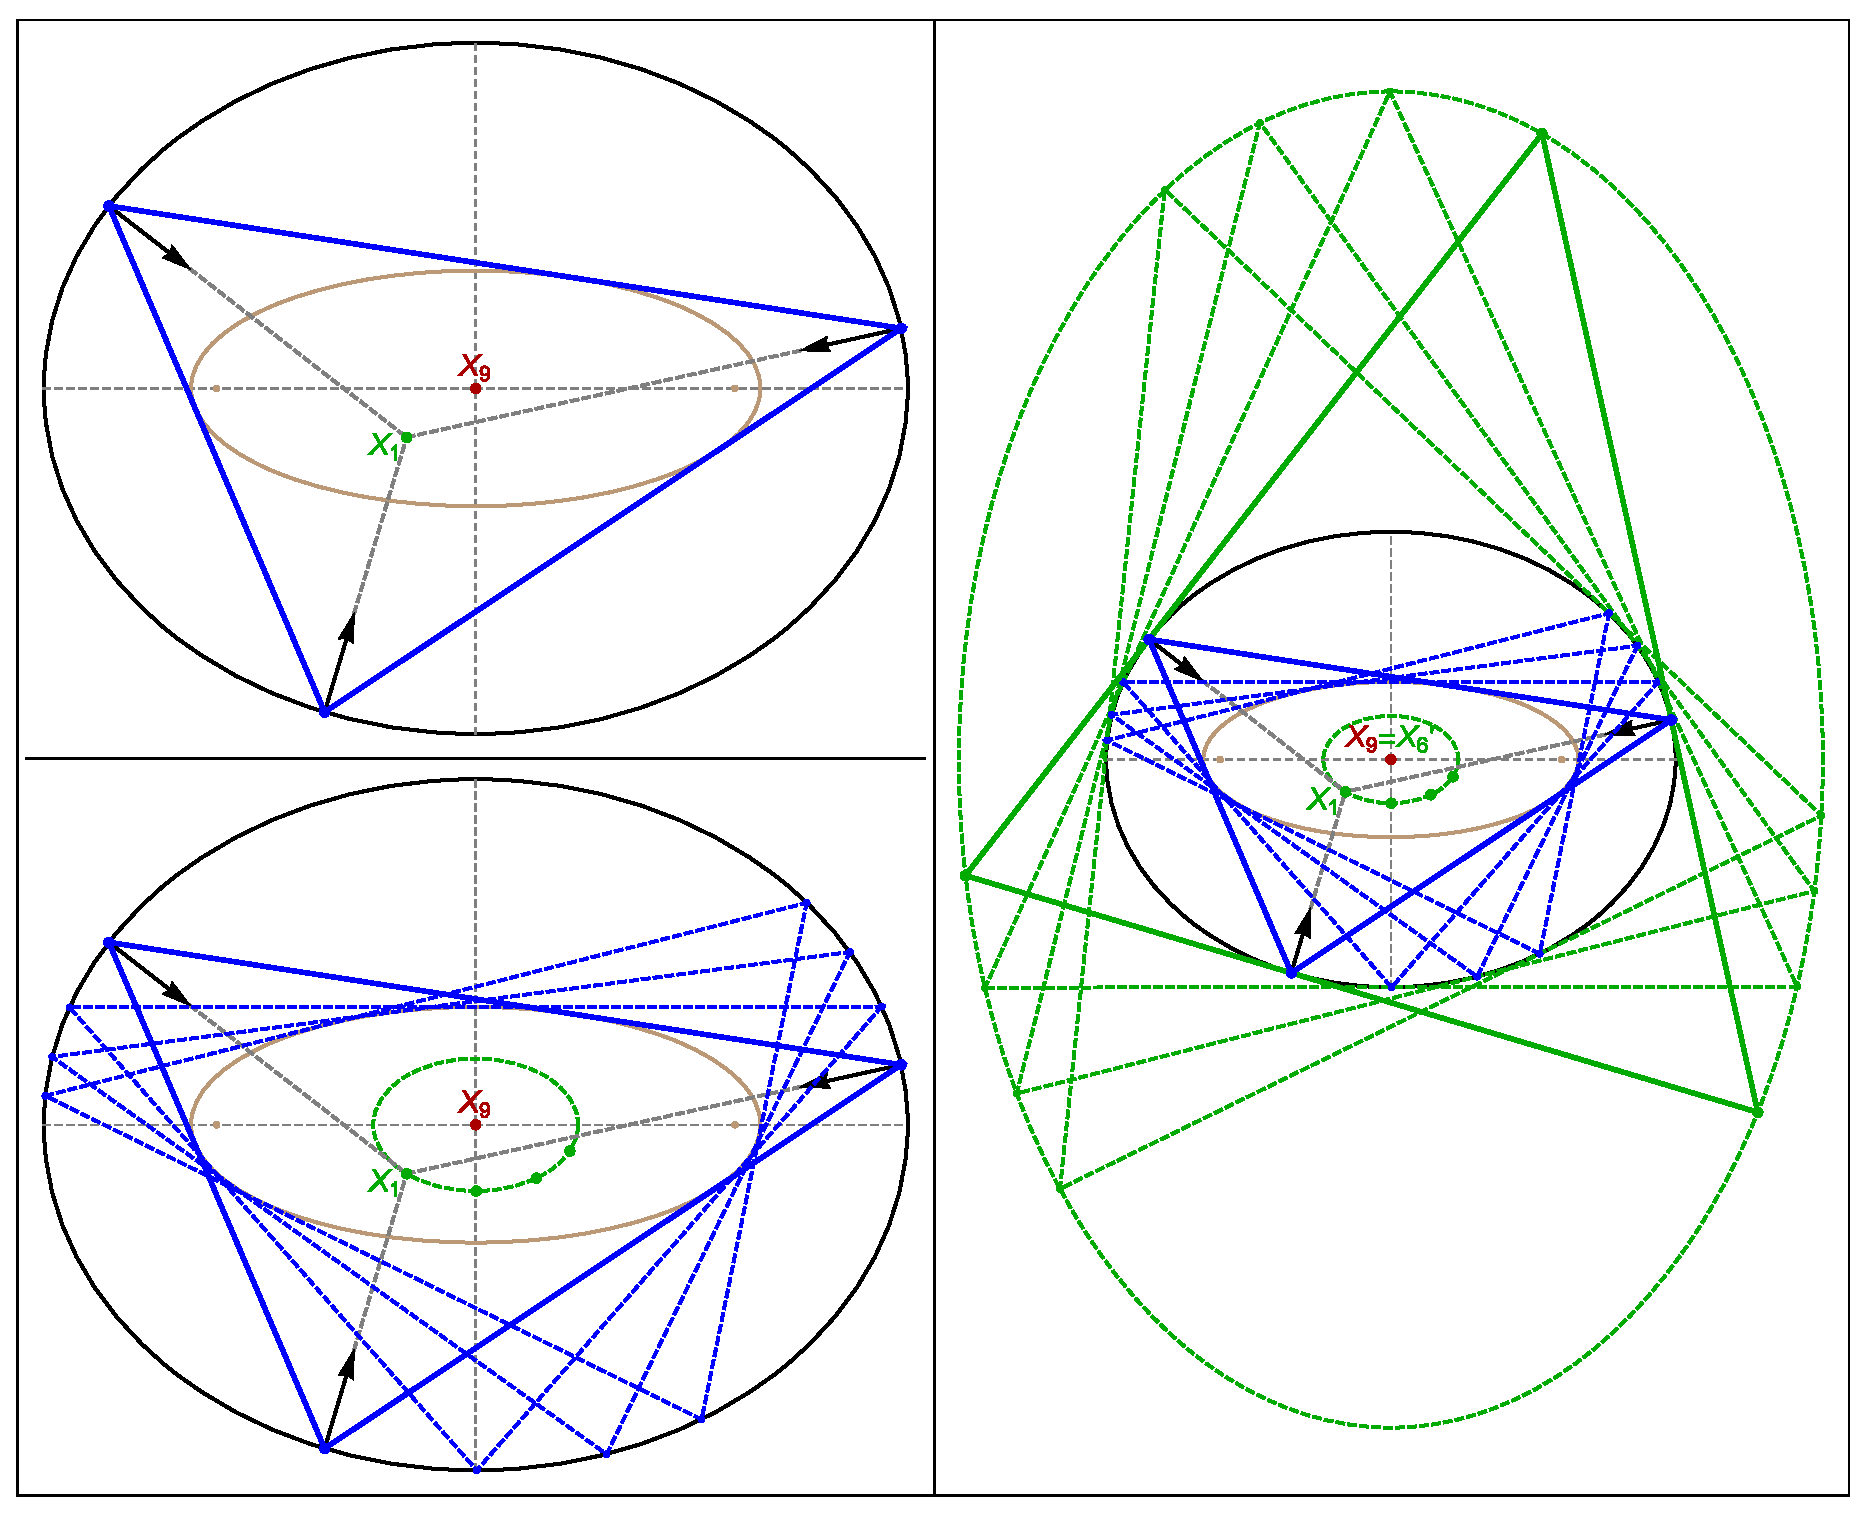
\includegraphics[width=\textwidth]{pics_02_010_billiard_grid}
    \caption{\textbf{Top Left:} An elliptic billiard 3-periodic (solid blue) is shown inscribed in an outer ellipse (black) and a confocal caustic (brown). Graves' theorem implies its internal angles will be bisected by ellipse normals (black arrows). Also shown is the incenter $X_1$ defined as the intersection of said bisectors. \textbf{Bottom Left:} Poncelet's porism implies a 1d family of such triangles exists. Some samples are shown (dashed blue). A classic invariant is  perimeter. The Mittenpunkt $X_9$ remains stationary at the center. The incenter $X_1$ sweeps an ellipse (dashed green). \textbf{Right:} The excentral triangle (solid green) has sides perpendicular to the bisectors. Over billiard 3-periodics, the excentral is of variable perimeter. Its vertices (known as the ``excenters'') also sweep an ellipse (dashed green) whose aspect ratio is the reciprocal of that of the incenter locus. The Symmedian point $X_6'$ of the excentral triangle coincides with $X_9$ of the reference and is therefore stationary. \href{https://bit.ly/3gWl3CI}{Live}}
    \label{fig:billiard-grid}
\end{figure}

An intriguing phenomenon is that over billiard 3-periodics, the locus of both incenter and the excenters are ellipses, as was initially detected experimentally (see an early \href{https://youtu.be/BBsyM7RnswA}{Video}). This was proved by \cite{olga14} and \cite{garcia2019-incenter}. Indeed, we haven't yet found another Poncelet pair where this is the case, see \cref{conj:07-incenter-excenter-loci}.

Referring to \cref{fig:billiard-grid}:

\begin{theorem}
Over billiard 3-periodics, the locus of the incenter $X_1$ and excenter are ellipses $\E_1$ and $\E_e$ concentric and axis-parallel with the confocal pair whose axes $(a_1,b_1)$ and $(a_e,b_e)$ are given by:
\begin{align*}
a_1 =& \frac{\delta-b^2 }{a},\;\;\;b_1=\frac{a^2-\delta}{b}\\ 
a_e= &\frac{{b}^{2}+\delta}{a},\;\;\;b_e=\frac{{a}^{2}+\delta}{b}
\end{align*}
Furthermore, $\E_1$ and $\E_e$ have reciprocal aspect ratios, i.e., $a_1/b_1=b_e/a_e$.
\label{thm:02-incenter-excenter}
\end{theorem}

\begin{proof}
It follows from the vertex parametrization in \cref{eq:02-p2} and the definition of incenter and excenters. We have that
\[X_1=\frac{s_1 P_1+s_2P_2+s_3P_3}{s_1+s_2+s_3}=
\frac{1}{L}(s_1P_1+s_2P_2+s_3P_3)\]
where $s_1=|P_2-P_3|$, $s_2=|P_1-P_3|$ and $s_3=|P_1-P_2|$.
A careful symbolic analysis shows that $\mathcal{E}_1(X_1)=0$. A similar analysis considering the excenters shows that the locus of the three points is the ellipse $\mathcal{E}_e$ stated.
\end{proof}

\noindent A more general treatment to the above is given in \cref{chap:07-n3-loci}.

\begin{corollary}
The pair $\{\mathcal{E},\mathcal{E}_e\}$ is Ponceletian.
\label{cor:02-excentral-billiard-poncelet}
\end{corollary}

\begin{proof}
Direct from Cayley condition
\[\frac{a}{a_e}+\frac{b}{b_e}=\frac{a^2}{b^2+\delta}+\frac{b^2}{a^2+\delta}= 1\]

\end{proof}

\section{A stationary point}
\label{sec:02-stationary}

The Mittenpunkt $X_9$ is a triangle center where lines from each excenter thru the side midpoint meet. Referring to \cref{fig:02-x9}:
\begin{theorem}
Over the family of 3-periodics in the elliptic billiard, $X_9$ is stationary at the common center.
\end{theorem}

An elegant syntethic proof was kindly contributed by \cite{olga19_mitten}:

\begin{proof}
Let $\E$ be the outer ellipse in the confocal pair, $O$. By definition, the Mittenpunkt $X_9$ is where lines from the excenters $E_i$ through the side midpoints $M_i$ concur. Notice each side is an ellipse chord between tangents to $\E$ seen from the $E_i$ (this is because in the confocal pair the excentral triangle is tangent to $\E$). Consider the image of lines $E_i M_i$ under an affine transform which sends $\E$ to a circle $\Cm'$, let $O'$ be its center. The transformed lines will pass through the midpoints of chords of $\Cm'$ between tangents seen from $E_i'$ (the affine image of $E_i$). By circular symmetry, such lines must also pass through $O'$, and therefore remain stationary. But $O'$ is the affine image of $O$, so the result follows.
\end{proof}

\begin{figure}
     \centering
    \includegraphics[width=\linewidth]{pics_02_020_mitten_proof.pdf}
     \caption{\textbf{Left}: 3-periodic billiard triangle (blue), its excentral triangle (green). The Mittenpunkt $X_9$ is the point of concurrence of lines drawn from the excenters through sides' midpoints $M_i$. \textbf{Right}: the affine image which sends the billiard to a circle. Lines from imaged excenters through sides' midpoints must pass through the origin. Since the latter is stationary, so must be its pre-image $X_9$, which is stationary at the billiard center.  % done
     \href{https://youtu.be/tMrBqfRBYik}{Video}}
     \label{fig:02-x9} 
\end{figure}

\section{Conserved Quantities}

Given a triangle, let $r$ and $R$ denote the radius of its incircle and circumcircle, known as the {\em inradius} and {\em circumradius}, respectively. Over billiard 3-periodics, note these two radii are variable. Referring to \cref{fig:radii}:

\begin{theorem}
$r/R$ is invariant over billiard 3-periodics and given by:
\begin{equation*}
\label{eqn:rovR}
\frac{r}{R}=\frac{2 (\delta-b^2)(a^2-\delta)}{c^4}.
\end{equation*}
\label{thm:02-confocal-rovR}
\end{theorem}

\begin{proof}
The following relation, found in \cite{johnson1960}, holds for any triangle:

\begin{equation*}
 r R=\frac{s_1s_2s_3}{2 L}, 
\end{equation*}

\noindent where $L=s_1+s_2+s_3$ is the perimeter, constant over billiard 3-periodics. Therefore:

\begin{equation}
\frac{r}{R}=\frac{1}{2L} \frac{s_1s_2s_3}{R^2}\cdot
\label{eqn:rovR-cas}
\end{equation}

Next, let $P_1=(a,0)$ be a vertex of an isosceles 3-periodic. Obtain a candidate expression for $r/R$. This yields \eqref{eqn:rovR} exactly. Using the vertex parametrization in \cref{eq:02-p2}, derive an expression for the square of the right-hand side of \eqref{eqn:rovR-cas} as a function of $x_1$ and subtract from it the square of \eqref{eqn:rovR}. In  \cite{garcia2020-new-properties}
it is shown $\left(s_1s_2s_3/R^2\right)^2$ is rational on $x_1$. For simplification, use $R=s_1 s_2 s_3/(4A)$, where $A$ is the triangle area. With a CAS, show said difference is identically zero for all $x_1\in(-a,a)$.
\end{proof}


\begin{figure}
    \centering
    \includegraphics[width=\textwidth]{pics_02_030_radii}
    \caption{The incircle (green), circumcircle (purple), and 9-point (Euler's) circle (pink) of a billiard triangle (blue). These are centered on $X_1$, $X_3$, and $X_5$, respectively. Their radii are the inradius $r$, circumradius $R$, and 9-point circle radius $r_9=2R$. Over the family, the ratio $r/R$ is invariant. In turn this implies an invariant sum of cosines. \href{https://bit.ly/337hvpf}{Live}}
    \label{fig:radii}
\end{figure}

Let $\theta_i$, $r$, $R$, and $A$ denote the ith internal angle, inradius, circumradius, and area of a reference triangle. Primed quantities refer to the excentral triangle. The relations below, appearing in  \cite{johnson1960},  hold for any triangle:

\begin{align}
\sum_{i=1}^{3}{\cos\theta_i}&=1+\frac{r}{R} \label{eqn:02-sum-cos} \\
\prod_{i=1}^{3}{\cos\theta_i'}&=\frac{r}{4R} \label{eqn:02-exc-prod-cos} \\
\frac{A}{A'}&=\frac{r}{2R} \label{eqn:02-area-ratio}
\end{align}

\begin{corollary}
Over billiard 3-periodics, also invariant are the sum of 3-periodic cosines, the product of excentral cosines, and the ratio of excentral-to-3-periodic areas.
\label{cor:02-rOvR}
\end{corollary}

Direct calculations yields an expression for the invariant sum of cosines in terms of elliptic billiard constants $J$ and $L$.

\begin{corollary}
$\sum_{i=1}^{3}{\cos\theta_i}=J L - 3$
\end{corollary}

At it will be seen later in \cref{chap:05-billiard}, the above generalizes to $J L -N$ for all $N$.

Let $P_i$ be a billiard 3-periodic vertex and $d_{j,i}=|P_i-f_j|$ its distance to billiard focus $f_j$. 

\begin{proposition}
 Over billiard 3-periodics, the following sum is invariant:
\[  \sum\frac{1}{d_{1,i}}=\sum\frac{1}{d_{2,i}}=\frac {{a}^{2}+{b}^{2}+\delta}{a{b}^{
2}}
\]
\label{prop:02-confocal-inv-spokes}
\end{proposition}

\begin{proof}
Direct computation with CAS using vertex parametrization given in \cref{sec:02-vertex-para}.
\end{proof}

Let $P=(x,y)$ be a point on an ellipse with semi-axes $a,b$. In \cite[Ellipse]{mw}, the curvature at $P$ is expressed both in terms of its coordinates and the distances $d_1,d_2$ to the foci as follows:

\begin{equation}
\kappa = \frac{1}{a^2 b^2} \left(\frac{x^2}{a^4}+\frac{y^2}{b^4}\right)^{-3/2} = \frac{a b}{(d_1 d_2)^{3/2}}
\label{eqn:02=curv}
\end{equation}

Let $\kappa_i$ denote the billiard ellipse curvature at vertex $P_i$ of a Poncelet 3-periodic. From the above and \cref{prop:02-confocal-inv-spokes} obtain:

\begin{corollary}
Over billiard 3-periodics, the following quantity is conserved:
\[ \sum_{i=1}^3{\kappa_i^\frac{2}{3}} =\frac{ a^2 + b^2 + \delta}{ (ab)^{\frac{4}{3}} }\]
\label{prop:02-confocal-curv-sum}
\end{corollary}

\section{An interpretation for \torp{$\delta$}{delta}}

The Darboux constant $\delta$ appearing above has a curious geometric interpretation. Recall the power of a point $Q$ with respect to a circle $\Cm=(C_0,R_0)$ is given by $|Q-C_0|^2-R_0^2$, see \cite[Circle Power]{mw}. Let $\Cm$ denote the (moving) circumcircle of billiard 3-periodic, and $O=X_9$ the billiard center.

\begin{proposition}
The power of $O$ with respect to $\Cm$ is constant and equal to $-\delta$.
\label{prop:02-delta}
\end{proposition}

\begin{proof}
Consider an isosceles billiard 3-periodic given by \cref{eq:orbita3-isosceles}.
	Its circumcircle will be centered at $C_0=[ {\frac { {b}^{2}-\delta}{2b}},0]$ with circumradius $R_0=\frac {{b}^{2}+\delta}{2b}.$
	Therefore, the power of the center of the ellipse with respect to the circumcircle is given by  
	$$|OC_0|^2-R_0^2=\left(\frac { {b}^{2}-\delta}{2b}\right)^2 - \left(\frac {{b}^{2}+\delta}{2b}\right)^2=-\delta.$$
	
	The stated invariance is confirmed with a CAS using the vertex parametrization in \cref{eq:02-p2}.  
%	\textcolor{red}{localizar depois}
\end{proof}




\section{Confocal Vertex Parametrization}

We describe two parametrizations for billiard 3-periodic vertices: (i) standard and (ii) Jacobi.

\subsection{Standard}
\label{sec:02-confocal-standard-param}

We call ``standard'' parametrization that where a first vertex $P_1(t)$ of the billiard 3-periodic is parametrized as $P_1(t)=[x_1,y_1]=[a\cos{t},b\sin{t}]$.

As derived in \cite{garcia2019-incenter}, $P_2=(x_2,y_2)/q_2$ and $P_3=(x_3,y_3)/q_3$ where:

 \begin{equation}
 \label{eq:02-p2}
 \aligned 
x_{2}=&-{b}^{4} \left(  \left(   a^2+{b}^{2}\right)\cos^{2}\alpha   -{a}^{2}  \right) x_1^{3}-2{a}^{6} \,\cos  \alpha  \sin   \alpha  \, y_1^{3}\\
&+{a}^{4} \left(  ({a
}^{2}-3\, {b}^{2}) \cos^{2} \alpha  +{b}^{2}
 \right) {x_1}\,y_1^{2}-2\,{a}^{4}{b}^{2} \cos \alpha  \,\sin  \alpha    x_1^{2}{y_1},
\\
y_{2}=& 2{b}^{6} \,\cos \alpha\sin \alpha\,   x_1^{3}-{
a}^{4}  \left(  \left(   a^2+{b}^{2}\right)\cos^{2}  \alpha  -{b}^{2}  \right)  y_1^{3}\\
&+  2\,{a}^{2} {b}^{4}\cos \alpha \sin
  \alpha \; {x_1} y_1^{2} +{b}^{4}\left(  ({b
 }^{2}-3\, {a}^{2}) \cos^{2} \alpha  +{a}^{2}
  \right) x_1^{2}{y_1}
\\
q_2=&{b}^{4} \left( a^2-(a^2-b^2)\cos^2  \alpha   \right)
x_1^{2}+{a}^{4} \left(  {b}^{2}+(a^2-b^2)\cos^2 \alpha  
 \right) y_1^{2}\\
 & - 2\, {a}^{2}{b}^{2} \left({a}^{2} -{b}^{2} \right)\cos \alpha\sin \alpha \; {x_1}\,{
y_1}.
\endaligned
%
\end{equation}

 \begin{equation} \label{eq:02-p3} \aligned 
x_{3}\; =& \; {b}^{4} \left( {a}^{2}- \left( {b}^{2}+{a}^{2} \right) 
 \cos^{2}\alpha\right)   x_1^{3}+2\, {a}^{6} 
 \cos \alpha\,\sin \alpha\, y_1^{3}\\
 &+{a}^{4} \left( 
  \cos^{2}  \alpha  \left( {a}^{2}-3\,{b}^{2}
 \right) +{b}^{2} \right) { x_1}\, y_1^{2}+2\,{a}^{4}{b}^{2} \cos  \alpha\sin \alpha\,   x_1^{2}{ y_1}
\\
y_{3} \;=&\; -2\, {b}^{6} \cos \alpha\sin \alpha\, x_1^{3}+
{a}^{4} \left( {b}^{2}- \left( {b}^{2}+{a}^{2} \right)   \cos^{2}  \alpha  \right)\,  y_1^{3}\\
& -2\,{a}^{2}  {b}^{4}\cos
 \alpha  \sin \alpha\,  x_1 y_1^{2}+
{b}^{4} \left( {a}^{2}+ \left( {b}^{2}-3\,{a}^{2} \right)  \left( \cos
 \alpha  \right) ^{2} \right) {{ x_1}}^{2}{ y_1},
\\
q_3 \;=& \; {b}^{4} \left( {a}^{2}- \left(a^2 -{b}^{2}  \right)   \cos^{2} \alpha   \right) x_1^{2}+{a}^{4} \left( {b}^{2}+ \left( a^2-{b}^{2}  \right)  \cos^{2} \alpha  \right)  y_1^{2}\\
&+2\,{a}^{2}{b}^{
2} \left( {a}^{2}-{b}^{2} \right) \cos \alpha \sin \alpha\, { x_1}\,{ y_1}.
\endaligned
%
\end{equation}
where:
\[\cos \alpha={\frac {a^2 b  \, \sqrt {-{a}^{2}-{b}^{2}+2\,\sqrt {{a}^{4}-{b}^{2}{c}^{2}}}}{{c}^{2}\sqrt {{a}^{4}-{c}^{2} x_1^{2}}}}=
\frac{  a^2 b^2 \, \sqrt {2\delta-{a}^{2}-{b}^{2}}} {c^2\sqrt{ a^4y_1^2 + b^4x_1^2}  } \]

Note that in \cref{sec:03-cap-vtx-param} we generalize the above to any concentric, axis-parallel pair.

\subsection{Jacobi's Universal Measure}
\label{sec:02-confocal-jacobi-param}

Under the standard parametrization, we can obtain the ``position'' $t$ of $P=[x,y]$ on an ellipse:

\[ t=\tan^{-1}{\frac{a y}{b x}}. \]

As shown in \cref{fig:02-jacobi-param}(top), when a first vertex $P_1(t)$ in the billiard 3-periodic is parametrized in the standard way, though its position is linear on the $t$ parameter, it will drive motions of the other two vertices $P_2(t)$ and $P_3(t)$ which are both distinct and non-linear. 

Fortunately, a uniform parametrization exists, which goes back to Jacobi, for all Poncelet families, based on the so-called ``universal measure'', which linearizes the Poncelet map, see \cite{koiller2021-spatial}. Specifically, vertices are obtained at fixed multiples of a constant $\Delta{u}$ in the argument of certain Jacobi elliptic functions. This parametrization, adapted to the elliptic billiard case, appears in \cite{stachel2021-billiards,stachel2021-billiards-param} and is reproduced below. First let's recall a few useful definitions. 

The  notation adopted below is as \cite{armitage-2006}. 

\begin{definition}
The incomplete elliptic integral of the first kind $K(\varphi,k)$ is given by:
\begin{equation}
K(\varphi,k)=\int_0^{\varphi}\frac{d\theta}{\sqrt{1-k^2 \sin^2\theta}}
\label{eqn:02-ellipticK}
\end{equation}
%\end{definition}

%\begin{definition}
The complete elliptic integral of the first kind $K(k)$ is simply $K(\pi/2,k)$.
\end{definition}

\begin{definition}
The elliptic sine $\text{sn}$, cosine $\text{cn}$, and delta-amplitude $\text{dn}$ are given by:
\begin{align*}
\text{sn}(u,k)&=\sin\varphi\\
\text{cn}(u,k)&=\cos\varphi\\
\text{dn}(u,k)&=\sqrt{1- k^2\sin^2\varphi}\\
\end{align*}
where $\varphi=\text{am}(u,k)$ is known as the amplitude, i.e., the upper-limit in the integral in \cref{eqn:02-ellipticK} such that $K(\varphi,k)=u$.
\end{definition}
A review of these functions appears in \cref{app:appD-jacobi-functions}.

\begin{remark}
Note to the reader: Mathematica (resp. Maple) expects $m=k^2$ (resp. $k$) as the second parameter to elliptic functions.

With this terminology the  Jacobi elliptic functions are defined    as follows:
\begin{align*}
K(\varphi,m)&=\int_0^{\varphi} \frac{dy}{\sqrt{1-m\sin^2y}}=u,\;\; \varphi=\text{am}(u,m)\\
%K(\varphi,k)=u\\ %
\sn(u,m)&=\sin\varphi,\; \cn(u,m)=\cos\varphi,\; dn(u,m)=\sqrt{1-m\sin^2\varphi}, \end{align*}

%As a note the reader, Maple accepts $k$ while Mathematica requires $m=k^2$ as the argument to elliptic functions.

%For example, in Maple we have: \[\sn(2,0.4)=\texttt{JacobiSN(2,.4)}=0.94569756\ldots\]
%and in Mathematica:

%\[ \sn(2,0.16)=\texttt{JacobiSN[2,.16]}=0.945698 \ldots \]
%and
%\[ \texttt{JacobiSN[2,.4]}=0.985090\ldots \]
\end{remark}

\begin{theorem}
A billiard orbit $P_i$ $(i=1,\ldots, N) $ of period $N$  with turning number $\tau$, where $\mathrm{gcd}(N,\tau) =1$,  is parametrized on $u$ with period $4K$ where:


\[ 
P_i=
%=\left[a\; \Jsn \left(u+\frac{4n\tau K}{N}, \frac{c}{a}\right), b\; \Jcn \left(u+\frac{4n\tau K}{N}, \frac{c}{a}\right)\right]\\
\left[-a\,\sn  \left(u+ i \Delta{u},  {m} \right) , b\,\cn  \left(u + i \Delta{u}, { m} \right)\right]
\]

where,
\[ m=k^2=\frac{a_c^2-b_c^2}{a_c^2},\;\;\Delta{u}=\frac{4\tau K}{N}\]
\[a= \sqrt{b^2+ a_c^2-b_c^2}, \;\; b=\frac{b_c}{\cn(\frac{\Delta{u}}{2}, m)}\]
\end{theorem}
\begin{proof} See \cite{stachel2021-billiards}.\end{proof}

A basic fact to obtain this parametrization is the following.

\begin{figure}
    \centering
    \includegraphics[width=\textwidth]{pics_02_040_param_jacobi.pdf}
    \caption{ Angular velocity $\vec v=\vec \omega\wedge \vec r$. } 
    \end{figure}
Referring to \cref{fig:02-velocidade-angular}:

\begin{proposition} 
Consider   segment of orbits $P_1P_2$ and $P_2P_3$  and contact points $Q_1$ and $Q_2$ with the caustic in an elliptic billiard. Let $\vec v$ the vector velocity of $P_2(t)$. Let $\vec r_1=Q_1-P_2$ and $\vec r_2=Q_2-P_2$. Then
\[ |\vec \omega_1|\;|\vec r_1|=|\vec \omega_2|\; |\vec r_2|\]
where $\vec v=\vec\omega_1\wedge r_1= \vec\omega_2\wedge \vec r_2$.

\label{fig:02-velocidade-angular}
\end{proposition}

\begin{proof} Let $\vec v=P_2'(t)$. From Graves's theorem, $|\vec r_1|+|\vec r_2|-\text{arc}(Q_1,Q_2)=\text{cte}$,  and therefore it follows that in decomposition of $\vec v=\vec v_{t_1}+\vec v_{n_1}=\vec v_{t_2}+\vec v_{n_2}$ we have that $|\vec v_{t_1}|=|\vec v_{t_2}|$ and  $|\vec v_{n_1}|=|\vec v_{n_2}|$. The result follows from the   definition of angular velocity. More details see \cite{stachel2021-billiards-param}.
\end{proof}
 
\textcolor{red}{ronaldo}
 
Since in this chapter we are considering billiard 3-periodics, so above $N=3$, and $\tau=1$. As shown in \cref{fig:02-jacobi-param}, under the Jacobi parametrization each of the 3 vertices of billiard 3-periodics follows the exact same curve, albeit with a 120-degree phase.

Recall the sum of cosines is constant for billiard 3-periodics. \cref{fig:02-jacobi-cos-param} shows how individual cosines follow either (i) 3-distinct curves, or (ii) the same exact curve (at different phases) if the parametrization is standard or Jacobi, respectively.

\begin{figure}
    \centering
    \includegraphics[width=\textwidth]{pics_02_050_parametrizations}
    \caption{The ``position'' $\theta_i$ (vertical axis) of a point on an ellipse with semi-axes $a,b$ vs the billiard 3-periodic parameter (horizontal axis). \textbf{Top:} vertex  under ``standard parametrization'', i.e., $P_1(t)=[a\cos{t},b\sin{t}]$. Notice while $P_1$'s position evolves linearly, those of $P_2$ and $P_3$ are different curves. \textbf{Bottom:} Said positions under Jacobi's parametrization. Notice the three positions are 120-degree delayed copies of one another.}. 
    \label{fig:02-jacobi-param}
\end{figure}

\begin{proof}
\textcolor{red}{ronaldo}
\end{proof}
\begin{figure}
    \centering
    \includegraphics[width=\textwidth]{pics_02_060_cos_parametrizations}
    \caption{The cosines $\cos(theta_i)$ of billiard 3-periodic internal angles for the standard (top) and Jacobi parametrizations (bottom). While in the former case the three curves are distinct, in the latter case all cosines follow the same curve at different phases.}
    \label{fig:02-jacobi-cos-param}
\end{figure}

\begin{exercise}\label{ex:21} Show that a pair of   ellipses $x^2/A^2+y^2/B^2=1$ and $x^2/a^2+y^2/b^2=1$ with semiaxes $(A,B)$ and $(a,b)$ ($A>a,\;B>b$) has a porism of pentagons (5-periodic orbits) then
\[\frac{a^3}{A^3}+\frac{b^3}{B^3}+\left(\frac{a}{A}+\frac{b}{B}\right)^2=1+\left(\frac{a}{A}+\frac{b}{B}\right)\left(1+\frac{ab}{AB}\right)\]\end{exercise}

\begin{exercise}\label{ex:22} Consider a quartic curve $q(x,y)=x^4+y^4-1=0$ and a family of circles $\mathcal{C}_r:  \; x^2+y^2-r^2=0$.

\noindent i) Determine $r$ such that there is  1d-family of triangles inscribed in the quartic $x^4+y^4=1$ and sides tangent to the circle $x^2+y^2=r^2$. Analyze   properties of this family of triangles. See   \cref{fig:darbouxq4c2}.

\noindent ii) Show that the square with vertices $[\pm \frac{1}{\sqrt[4]{2}},\pm \frac{1}{\sqrt[4]{2}}]$ is inscribed in $ q(x,y)=0$ and its sides are tangent to the circle $x^2+y^2=\frac{\sqrt{2}}{2}.$ In this case show that there is no porism of Poncelet associated to the algebraic curves. See \cref{fig:period4darboux}.

\begin{figure}
    \centering
    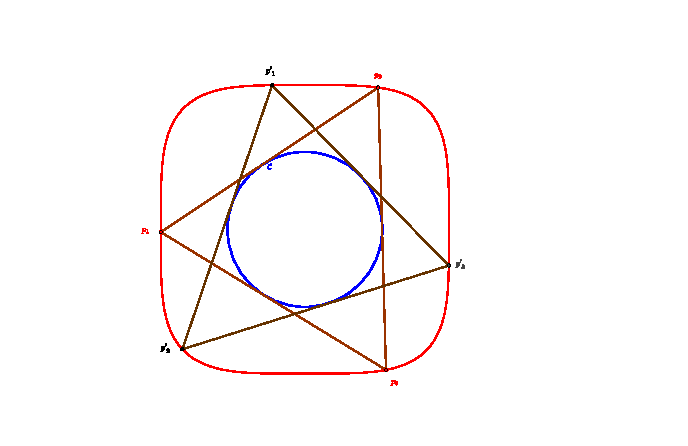
\includegraphics[scale=0.6]{pics_tex/darboux_Q4_C2.pdf}
    \caption{Porism of triangular orbits in a pair of a quartic and a circle.}
    \label{fig:darbouxq4c2}
\end{figure}


\begin{figure}
    \centering
     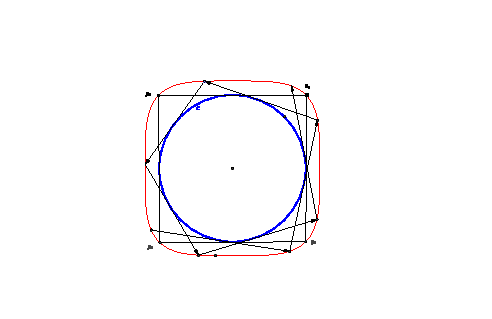
\includegraphics[scale=1]{pics_tex/periodo4_darboux_Q4_C2.pdf}
    \caption{Non existence of a porism of quadrilateral orbits in a pair of a quartic and a circle.}
    \label{fig:period4darboux}
\end{figure}

\end{exercise}


\begin{exercise}\label{ex:23} 

\end{exercise}


\begin{exercise}\label{ex:24}

\end{exercise}
\section{Research Questions}

\begin{question}
Recall the extouch triangle has vertices at the points of contact of the excircles with a triangle's sidelines \cite[Extouch triangle]{mw}. 
In \cref{chap:05-confocal-loci} we show that the vertices of the extouch triangles of billiard 3-periodics coincide with the caustic touchpoints, see it 
\href{https://bit.ly/33PufRv}{Live}. Show that said extouch family is also Ponceletian and concentric with the elliptic billiard; derive expressions for the semi-axes of its elliptic caustic. Is its center a triangle center? 
\label{que:02-extouch}
\end{question}


\chapter{Properties of N=3 Poncelet Families}
\label{chap:03-n3-properties}
\section{History of Results}
\label{sec:03-history}
Early videos 2011 com Jair Koiller \cite{dsr_vid11incenter,dsr_vid11e}, proof by complexification \cite{olga14}, proof by Affine Curvature \cite{garcia2019-incenter}, circumcenter \cite{corentin2021-circum}. Schwartz \cite{schwartz2016-com}, Circumcenter of Mass \cite{sergei2014-circumcenter-of-mass}.

\section{Combo}
\section{Triangle Centers}

\section{Some Concentric N=3 Families}

\section{Elliptic Loci in Generic Pairs}

\section{Exercises}

\begin{exercise}
blablabla
\end{exercise}

\section{Videos}


Referring to Figure~\ref{fig:nonconcentric-xns}:

\begin{figure}
     \centering
     \includegraphics[width=.8\textwidth]{pics_03_010_n3_nonconcentric_conics.eps}
     \caption{A 3-periodic is shown interscribed between two non-concentric, non-aligned ellipses (black). The loci of $X_k$, $k=2,3,4,5,20$ (and many others) are elliptic. Those of $X_2$ and $X_4$ are axis-aligned with the outer ellipse. Furthermore, the centers of all elliptic loci are collinear (magenta line).}
     \label{fig:nonconcentric-xns}
 \end{figure}
 
\section{Locus of Incenter and Excenters}\label{sec:inc_excenter}

\begin{theorem}
Over the family of 3-periodics interscribed in a generic nested pair of ellipses (non-concentric, non-axis-aligned),
if $\X\ab$ is a fixed linear combination of $X_2$ and $X_3$, i.e., $\X\ab=\alpha X_2+\beta X_3$ for some fixed $\alpha,\beta\in\mathbb{C}$, then its locus is an ellipse. 
\label{thm:ellipse-locus}
\end{theorem}


\begin{theorem}
Over 3-periodics in the elliptic billiard (confocal pair) the locus of the incenter $X_1$ is an ellipse given by 
$x^2/a_1^2+y^2/b_1^2=1$, where
	\begin{equation*}\label{eq:Eint}\aligned
	a_1 =& \frac{\delta-b^2 }{a},\;\;\;
	%
	b_1  =   \frac{a^2-\delta}{b},\;\;\; \delta=\sqrt{a^4-a^2b^2+b^4}.
	%
	\endaligned
	\end{equation*}
	
	The locus of the Excenters (triangle formed by the intersection of external bisectors) is an ellipse with axes:
 
\begin{equation*}
 a_e=\frac{{b}^{2}+\delta}{a},\;\;\; 
 b_e=\frac{{a}^{2}+\delta}{b}
\end{equation*}
 
\noindent Notice it is similar to the $X_1$ locus, i.e., $a_1/b_1=b_e/a_e$.
\end{theorem}

A list of the elliptic loci of centers in the $X_{1}$ to $X_{200}$ range can be found \href{https://dan-reznik.github.io/why-so-many-ellipses/}{here}.

\section{Future Work}

\begin{conjecture}
The locus of the incenter is an ellipse if and only if the Poncelet ellipse pair is confocal.
\end{conjecture}

Let  $\mathbb{T } = \{ z\in \mathbb{C}: |z| = 1\} $ the unit circle and $\mathbb{D} = \{ z\in\mathbb{C} : |z| < 1\} $ the open unit disk
bounded by $\mathbb{T }.$

\begin{lemma}
If $u,v,w\in\mathbb{C}$ and $\lambda$ is a parameter that varies over the unit circle $\T\subset\mathbb{C}$, then the curve parametrized by
\[ F(\lambda)=u \lambda+ \frac{v}{\lambda}+w \]
is an ellipse centered at $w$, with semiaxis $|u|+|v|$ and $\big||u|-|v|\big|$, rotated with respect to the horizontal axis of $\mathbb{C}$ by an angle of $(\arg u+\arg v)/2$.
\label{lem:ell-param}
\end{lemma}
\begin{proof}

\end{proof}


Consider the Moebius map $M_{z_0}=(z_0-z)/(1-\overline{z_0} z)$ and the Blaschke product of degree 3 given by   $B=M_{z_0} M_{z_1} M_{z_2}$.
\begin{theorem}
Let $B$ be a Blaschke product of degree 3 with
zeros $0, f, g.$ For $\lambda \in \mathbb{T}$, let $z_1, z_2, z_3 $ denote the three distinct solutions to $ B(z) = \lambda$. Then the
lines joining $z_j$ and $z_k$, $(j \ne k)$ are tangent to the ellipse given by
\[|w - f| + |w - g| = |1 -   \overline{f}   g |.\]
\end{theorem}

\begin{theorem}
 Given two points $f,g\in\mathbb{D}$. Then there exists a unique conic $\mathcal{E}$ with the foci
$f,g$   which is 3-Poncelet caustic with respect to $\mathbb{T}$. Moreover, $\mathcal{E}$ is an ellipse. That ellipse is
the Blaschke ellipse with the major axis of length $|1-\overline{f}g|.$
\end{theorem}

Consider the parametrization of a triangular orbit $\{z_1,z_2,z_3\}$ as given in \cite{helman2021-power-loci}.
Let also the  affine transformation
$T(z)=pz+q\ol z$.
\begin{definition}[Blaschke's Parametrization]
\begin{align*}
    \sigma_1:=z_1+z_2+z_3=& f+g+\l\ol f \ol g =\alpha\\
    \sigma_2:=z_1 z_2+z_2 z_3+z_3 z_1=& f g+\l(\ol f+\ol g) =\beta\\
    \sigma_3:=z_1 z_2 z_3=& \l
\end{align*}
where $f,g$ are the foci of the inner ellipse and $\l\in\T$ is the varying parameter.
\label{def:bla}
\end{definition}
\begin{proposition}\label{prop:X1c}
Over Poncelet 3-periodics in the pair with an outer circle and an ellipse in generic position, the locus $X_1$ given by:
\begin{align*}
  X_1:&\;z^4 - 2(( \bar{f} + \bar{g}) \lambda +  f g) z^2 + 8   \lambda z\\
  &+ (\bar{f} - \bar{g})^2 \lambda^2 +2 (  |f|^2 g +   f |g|^2 - 2 f - 2 g) \lambda + f^2 g^2=0\\
  \;&:\;  z^4 - 2\beta  z^2+ 8\lambda z+  (\beta^2-4\alpha\lambda) =0
\end{align*}
\end{proposition}

\begin{proof} The incenter of a triangle with vertices $\{z_1,z_2,z_3\}$ is given by:
\begin{align*}
    X_1&=\frac{\sqrt{a}\;z_1+\sqrt{b}\;z_2+\sqrt{c}\;z_3}{\sqrt{a}+\sqrt{b}+\sqrt{c}}\\
    a&=|z_2-z_3|^2, \; b=|z_1-z_3|^2, \;\; c=|z_2-z_1|^2
\end{align*}
Using that $z_i\in \T$ it follows that
\[a=2-(\frac{z_3}{z_2}+\frac{z_3}{z_2}),\;\; b=2-(\frac{z_1}{z_3}+\frac{z_3}{z_1}),\;\;c=2-(\frac{z_1}{z_2}+\frac{z_2}{z_1})\]
Eliminating the square roots in  the equation $X_1-z=0$ and using the relations  $\sigma_i$ (i=1,2,3) given in Blaschke's parametrization the result follows.
\end{proof}

\begin{proposition}
\label{prop:X1g}
Over Poncelet 3-periodics in a generic nested ellipse pair, the locus of $X_1$ is given by the following sextic polynomial in $z,\lambda$:
{\small
\begin{align*}
X_1&: \;{\lambda}^{2} \left( p^2-q^2 \right) {
z}^{4}+4\,\lambda\, \left( \alpha\,\lambda\,p q^2  - q\,{
\lambda}^{2}p^{2}-\beta\,p^2\,q+p\,q^{2} \right) {z}^{3}\\
&+  ( 4\,\alpha\,{
\lambda}^{3}p^{3} q-4\,{\alpha}^{2}{\lambda}^{2}p^{2}q^2 +2\,\alpha\,\beta\,\lambda\,p^{3}
\,q-2\,\alpha\,\beta\,\lambda\,pq^{3} -2\,\beta\,{\lambda}^{2
}p^{4}+6\,\beta\,{\lambda}^{2}p^{2}q^2\\
&-6\,\alpha\,
\lambda\,p^2\,q^{2}+2\,\alpha\,\lambda\,q^{3} q+4\,{
\beta}^{2}p^2\,q^{2}  
  +6\,{\lambda}^{2}p^{3} \,q
 -6\,{
\lambda}^{2} p q^{3}  -4\,\beta\,p\,q^{3}  ) {z}^{
2}\\
&+ ( 4 q (\alpha^2\beta p^2 q^2 + 2\alpha^2 p^2  p q - \alpha^2 p q^3 + \beta^2 p^4 - 2\beta^2 p^2 q^2+ 4\beta p q^3 - p^2 q^2 - 2 q^4)\lambda \\
&- 4\alpha  p q^2 (\beta^2 p^2 - q^2) - 4 p^3 (\beta p  q - 2 p^2 - q^2)\lambda^3 - 16\alpha\lambda^2 p^4   q ) z\\
   & -\lambda^2 (4 \alpha \lambda - \beta^2) p^6 + 4 p^5 q \lambda^4 + 2 \lambda (4 \alpha^2 \lambda - \alpha \beta^2 - 3 \beta \lambda) p^5 q   - \lambda^2 (8 \alpha \lambda - 3 \beta^2) p^4 q^2 \\
   &+ (\alpha^2 \beta^2 -4 \alpha^3 \lambda  + 4 \alpha \beta \lambda + 5 \lambda^2) p^4 q^2 + 2 \lambda (2 \alpha^2 \lambda - \alpha \beta^2 + \beta \lambda) p^3 q^3 \\
   &+ (2 \alpha^2 \beta - 2 \alpha \lambda - 4 \beta^2) p^3 q^3 - (\alpha^2 \beta^2 + 4 \alpha \beta \lambda - 4 \beta^3 + 5 \lambda^2) p^2 q^4 + ( 8 \beta-3 \alpha^2 ) p^2 q^4 \\
   &+ (2 \alpha^2 \beta + 6 \alpha \lambda - 8 \beta^2) p q^5 - 4 q^5 p + ( 4 \beta-\alpha^2 ) q^6=0
\end{align*}
}
\end{proposition}

\begin{proof} Let $p,q\in \mathbb{R}$. Consider the affine transformation
$T(z)=pz+q\ol z$ and set $w_i=T(z_i)$. The proof is similar to that given in \cref{prop:X1c}.  
\end{proof}

\begin{proposition} In the confocal pair the locus $X_1$ is defined by:
\[2\,ab{\lambda}^{2}{z}^{2}+2\,\lambda\, \left( {a}^{3}{\lambda}^{2}-{b}
^{3}{\lambda}^{2}-{a}^{3}-{b}^{3} \right) z+{c}^{2} \left( {c}^{2}{
\lambda}^{4}-2\,ab{\lambda}^{2}-{c}^{2} \right)=0 \]
\label{prop:X1q2} 
\end{proposition}

\begin{proof}
We have that
\[f={\frac {1}{c}\sqrt {-{a}^{2}-{b}^{2}+2\,\delta}}, \;\; g= -{\frac {1}{c}\sqrt {-{a}^{2}-{b}^{2}+2\,\delta}}\]

\end{proof}

\begin{corollary}
The locus $X_1$ is the ellipse with semiaxes given by $a_1=(a^2-\delta)/b$ and $b_1=(\delta-b^2)/a.$

%\[z= {\frac { \left( a-b \right)  \left(\delta -{a}^{2}-ab-{b}^{2}
 %\right) \lambda}{2\,ab}}-{\frac { \left( a+b %\right)  \left(  \delta-{a}^{2}
%+ab-{b}^{2} \right) }{2\,ab\lambda}}\]
 
\end{corollary}

\begin{proof}
The quartic polynomial is factorizable as $p_1p_2$, where
\begin{align*}
    p_1&=z-\left({\frac { \left( a-b \right)  \left( -{a}^{2}-a b-{b}^{2}+\delta
 \right) \lambda}{2\,a b}}-{\frac { \left( a+b \right)  \left( -{a}^{2}
+a b-{b}^{2}+\delta \right) }{2\,a b\lambda}}\right)
\\
    p_2&=2 a b \lambda^2 z^3 - ((a - b) (a^2 + 3 a b + b^2 + \delta) \lambda^3 - (a + b) (a^2 - 3 a b + b^2 + \delta) \lambda) z^2\\
    &+ 6 a b  (a^2 - b^2) \lambda^2 z + (a + b)^3 (a^2 - a b + b^2 + \delta) \lambda^3 - (a - b)^3 (a^2 + a b + b^2 + \delta) \lambda
\end{align*}
Follows directly from  \cref{lem:ell-param} and  \cref{prop:X1q2}.
\end{proof}

\cite{schwartz2016-com}

\begin{conjecture}
Over 3-periodics interscribed between two ellipses in general position, the locus of a triangle center $X_k$ is an ellipse if and only if $X_k$ is a fixed linear combination of $X_3$ and $X_4$.
\end{conjecture}

\chapter{Analyzing Loci of N=3 Poncelet Families}
\label{chap:04-n3-loci}
%In the previous chapter we restricted ourselves to observing various interesting locus-related phenomena in the confocal pair. 
Namely, we attempt to answer the following related questions:

\begin{itemize}
    \item When are loci algebraic?
    \item What is the type of curve for the locus of the incenter (and excenters) in a generic concentric, axis-parallel (CAP) pair?
    \item In \cite{sergei2016-com} it is shown that over Poncelet N-periodics in a generic pair of conics, the locus of vertex and area centroids is an ellipse. For triangles, both points collapse to $X_2$. Given 3-periodics in a generic pair of ellipses, when is the locus of some triangle center an ellipse? To answer we will use technique based on Blaschke products \cite{daepp-2019}, review below;
    \item We consider the special case of 3-periodics in a pair with a circumcircle, showing that many such loci are circles.
\end{itemize}

\section{When are Loci Algebraic?}
\label{sec:04-rational-trilinears}
\input{chap_04/04_020_algebraic_loci}

\section{Review: Blaschke Products}
\label{sec:04-blaschke}
\input{chap_04/04_050_blaschke}

\section{Locus of the Incenter in a CAP pair}
\label{sec:04-proof_theorem}
\input{chap_04/04_055_proof_theorem_incenter_excenter}

\section{Loci in Generic Nested Ellipses}
\label{sec:04-loci}

 In this Section we prove the locus of a given fixed linear combination of $X_2$ and $X_3$ is an ellipse. We will use Blaschke products since, as shown in \cref{fig:04-affine}, a generic non-concentric pair is always the affine image of a pair with circumcircle.
 
 \begin{figure}
    \centering
    \includegraphics[width=\textwidth]{pics_04_030_affine_circumcircle.eps}
    \caption{Affine transformation that sends a generic ellipse pair and its 3-periodic family (left) to a new pair with circumcircle (right). We parametrize the 3-periodic orbit with vertices $z_i$ in the circumcircle pair using the foci of the latter's caustic $f$ and $g$, and then apply the inverse affine transformation to get a parametrization of the vertices $P_i$ of the original Poncelet pair. \href{https://youtu.be/6xSFBLWIkTM}{Video}}
    \label{fig:04-affine}
\end{figure}

\begin{figure}
    \centering
    \includegraphics[width=.8\textwidth]{pics_04_010_n3_nonconcentric.eps}
    \caption{A pair of ellipses in general position which admits a Poncelet 3-periodic family (blue). Let the outer one be centered at the origin $O$. Their major axes are tilted by $\theta$, and their centers displaced by $O_c=(x_c,y_c)$. \href{https://youtu.be/bjHpXVyXXVc}{Video}}
    \label{fig:04-n3-nonconcentric}
\end{figure}

Consider the generic pair of nested ellipses $\E=(O,a,b)$ and $\E_c=(O_c,a_c,b_c.\theta)$ in Figure~\ref{fig:04-n3-nonconcentric}. Let s$\theta$, c$\theta$ denote the sine and cosine of $\theta$, respectively. Define $c_c^2=a_c^2-b_c^2$. The Cayley condition for the pair to admit a 3-periodic family is given by:

{\small
\begin{align}
&{b}^{4}x_c^{4}+2\,{a}^{2}{b}^{2}x_c^{2}y_c^{2}+
 \left(  2 c_c^2  \left( -{b}^{2}({a}^{2}+{b}^{2} )\right)  \text{c}\theta^2  - 2\left(  \,b ^{2}- \,b_c
^{2} \right) {b}^{2}{a}^{2}-2\,{b}^{4}b_c^{2} \right)x_c
^{2} \label{eqn:cayley}\\
&-8\,{a}^{2}{b}^{2}x_c\,{  y_c}\,c_c^2 
\text{s}\theta\text{c}\theta  +{a}^{4}y_c^{4} + \left(  2 c_c^2 a^2 \left(
{a}^{2}+{b}^{2}  \right)\text{c}\theta^2  
 -2 \left(  \,b_c^{2}+{b}^{2} \right) {a}^{4}+2
\,{a}^{2}{b}^{2}b_c^{2} \right) y_c^{2} \nonumber\\
&+ c_c^4  c^4  \left( \text{c}\theta^4-2\, c_c^2 c^2
  \left( {a}^{2} a_c^{2}-{b}^{2}{a}^{2}+
b_c^{2}{b}^{2} \right) \text{c}\theta^2 \right. \nonumber\\
 &+ \left( a a_c+a b-b b_c \right)  \left( a a_c
-a b -b b_c \right)  \left( a a_c+a b+b b_c \right)  \left( a
a_c-a b+b b_c \right) = 0\nonumber
\end{align}
}

%A related result is that the locus of the circumcenter-of-mass \cite{sergei2014-circumcenter-of-mass}, a generalization of $X_3$ for $N>3$ is also an ellipse.

Referring to Figure~\ref{fig:04-nonconcentric-xns}:

\begin{theorem}
Over the family of 3-periodics interscribed in an ellipse pair in general position (non-concentric, non-axis-aligned),
if $\X\ab$ is a fixed linear combination of $X_2$ and $X_3$, i.e., $\X\ab=\alpha X_2+\beta X_3$ for some fixed $\alpha,\beta\in\mathbb{C}$, then its locus is an ellipse. 
\label{thm:04-ellipse-locus}
\end{theorem}

\begin{proof}
Consider a general $N=3$ Poncelet pair of ellipses that forms a 1-parameter family of triangles. Without loss of generality, by translation and rotation, we may assume the outer ellipse is centered at the origin and axis-aligned with the plane $\R^2$, which we will also identify with the complex plane $\mathbb{C}$. Let $a,b$ be the semi-axis of the outer ellipse, and $a_c,b_c$ the semi-axis of the inner ellipse, as usual. 

Referring to Figure~\ref{fig:04-affine}, consider the linear transformation that takes $(x,y)\mapsto(x/a,y/b)$. This transformation takes the outer ellipse to the unit circle $\T$ and the inner ellipse to another ellipse. Thus, it transforms the general Poncelet $N=3$ system into a pair where the outer ellipse is the circumcircle, which we can parametrize using Blaschke products \cite{daepp-2019}. In fact, to get back to the original system, we must apply the inverse transformation that takes $(x,y)\mapsto(a x,b y)$. As a linear transformation from $\mathbb{C}$ to $\mathbb{C}$, we can write it as $L(z):=p z+q \ol{z}$, where $p:=(a+b)/2, q:=(a-b)/2$.

Let $z_1,z_2,z_3\in\T\subset\mathbb{C}$ be the three vertices of the circumcircle family, parametrized as in \cref{def:bla}, and let $v_1:=L(z_1),v_2:=L(z_2),v_3:=L(z_3)$ be the three vertices of the original general family. The barycenter $X_2$ of the original family is given by $(v_1+v_2+v_3)/3$, and the circumcenter $X_3$ is given by \cite{stackexchange-x3a}:

\[
    X_3=\left|
        \begin{array}{ccc}
          v_1 & |v_1|^2 & 1 \\
          v_2 & |v_2|^2 & 1 \\
          v_3 & |v_3|^2 & 1
        \end{array}
      \right| \Bigg/
     \left|
        \begin{array}{ccc}
          v_1 & \overline{v_1} & 1 \\
          v_2 & \overline{v_2} & 1 \\
          v_3 & \overline{v_3} & 1
        \end{array}
      \right|
\]

Since $\ol{z_1}=1/z_1,\ol{z_2}=1/z_2,\ol{z_3}=1/z_3$, we can write $v_1,v_2,v_3$ as rational functions of $z_1,z_2,z_3$, respectively. Thus, both $X_2$ and $X_3$ are symmetric rational functions on $z_1,z_2,z_3$. Defining $\X\ab=\alpha X_2+\beta X_3$, we have consequently that $\X\ab$ is also a symmetric rational function on $z_1,z_2,z_3$. Hence, we can reduce its numerator and denominator to functions on the elementary symmetric polynomials on $z_1,z_2,z_3$. This is exactly what we need in order to use the parametrization by Blaschke products.

In fact, we explicitly compute:
\[  \X\ab= \frac{p^2 q \left(\sigma_2 (\alpha +3 \beta )+3 \beta  \sigma_3^2\right)+\alpha  p^3 \sigma_1 \sigma_3-p q^2 (3 \beta +\sigma_1 \sigma_3 (\alpha +3 \beta ))-\alpha  q^3 \sigma_2}{3 \sigma_3 (p-q) (p+q)}\]
where $\sigma_1,\sigma_2,\sigma_3$ are the elementary symmetric polynomials on $z_1,z_2,z_3$.

Let $f,g\in\mathbb{C}$ be the foci of the inner ellipse in the circumcircle system. Using Definition~\ref{def:bla}, with the parameter $\l$ varying on the unit circle $\T$, we get:

\begin{equation}
\X\ab= u \l+v\frac{1}{\l}+w
\label{eqn:xi-param}
\end{equation}

\noindent where:

\begin{align*}
    u:=&\frac{p \left(\ol{f} \ol{g} \left(\alpha  p^2-q^2 (\alpha +3 \beta )\right)+3 \beta  p q\right)}{3 (p-q) (p+q)}\\
    v:=&\frac{\beta  p q (q-f g p)}{(q-p) (p+q)}+\frac{1}{3} \alpha  f g q\\
    w:=&\frac{q \left(\ol{f}+\ol{g}\right) \left(p^2 (\alpha +3 \beta )-\alpha  q^2\right)+p (f+g) \left(\alpha  p^2-q^2 (\alpha +3 \beta )\right)}{3 (p-q) (p+q)}
\end{align*}

By   \cref{lem:ell-param}, this is the parametrization of an ellipse centered at $w$, as desired. As in  \cref{lem:ell-param}, it is also possible to explicitly calculate its axis and rotation angle, but these expressions become very long.
\end{proof}

In \cref{thm:04-ellipse-locus} a linear combination of $X_2$ and $X_3$ was considered in terms of complex parameters $\alpha,\beta$. Below this result is specialized to the case of an affine combination of said centers in terms of a real parameter $\gamma$.

\begin{corollary}
Over the family of 3-periodics interscribed in an ellipse pair in general position (non-concentric, non-axis-aligned),
if $\X_\gamma$ is a real affine combination of $X_2$ and $X_3$, i.e., $\X_\gamma=(1-\gamma) X_2+\gamma X_3$ for some fixed $\gamma\in\R$, then its locus is an ellipse. Moreover, as we vary $\gamma$, the centers of the loci of the $\X_\gamma$ are collinear.
\end{corollary}

\begin{proof}
Apply   \cref{thm:04-ellipse-locus} with $\alpha=1-\gamma, \beta=\gamma$ to get the elliptical loci. As in the end of the proof of  \cref{thm:04-ellipse-locus}, the center of the locus of $\X_\gamma$ can be computed explicitly as 
\begin{gather*}
    w=w_0+w_1 \gamma \text{, where}\\
    w_0=\frac{1}{3} \left(q \left(\ol{f}+\ol{g}\right)+p (f+g)\right)\\
    w_1=\frac{q \left(2 p^2+q^2\right) \left(\ol{f}+\ol{g}\right)-p (f+g) \left(p^2+2 q^2\right)}{3 (p-q) (p+q)}
\end{gather*}
As $\gamma\in\R$ varies, it is clear the center $w$ sweeps a line.
\end{proof}

We proved that all of the following triangle centers have elliptic loci in the general N=3 Poncelet system, including the barycenter, circumcenter, orthocenter, nine-point center, and de Longchamps point (reflection of the orthocenter  about the circumcenter of a triangle):

\begin{observation}
Amongst the 40k+ centers listed on \cite{etc}, about 4.9k triangle centers lie on the Euler line \cite{etc-central-lines}. Out of these, only 226 are fixed affine combinations of $X_2$ and $X_3$. For $k<1000$, these amount to $X_k,k=${\small 2, 3, 4, 5, 20, 140, 376, 381, 382, 546, 547, 548, 549, 550, 631, 
632}.
\label{obs:affine-euler-line}
\end{observation}

\begin{figure}
     \centering
     \includegraphics[width=\textwidth]{pics_04_020_n3_nonconcentric_loci.eps}
     \caption{A 3-periodic is shown interscribed between two nonconcentric, non-aligned ellipses (black). The loci of $X_k$, $k=2,3,4,5,20$ (and many others) remain ellipses. Those of $X_2$ and $X_4$ remain axis-aligned with the outer one. Furthermore the centers of all said elliptic loci are collinear (magenta line). \href{https://youtu.be/p1medAei_As}{Video}}
     \label{fig:04-nonconcentric-xns}
 \end{figure}
 
%\begin{corollary}
%The elliptic loci of $X_2$, $X_3$ and $X_4$ are given by:
%\[ \textcolor{red}{mark} \]
%\textcolor{red}{these will be hard to get explicitly}
%\end{corollary}
 
\begin{observation}\label{obs:X2X4}
The elliptic loci of $X_2$ and $X_4$ are axis-aligned with the outer ellipse.
\end{observation} 

%\begin{figure}
%    \centering
%    \includegraphics[width=.7\textwidth]{pics_04_040_n3_nonconcentric_circular_caustic.eps}
%    \caption{A 3-periodic (blue) is shown inscribed in an outer ellipse and an inner non-concentric circle centered on $O_c$. The loci of both circumcenter (solid red) and Euler center (solid green) are ellipses whose major axes pass through $O_c$. \href{https://youtu.be/w7sZ5O8k4xU}{Video}}
%    \label{fig:04-circular-caustic}
%\end{figure}

Experimental evidence suggests:

\begin{conjecture}
Over 3-periodics interscribed between two ellipses in general position, the locus of a triangle center $X_k$ is an ellipse if and only if $X_k$ is a fixed linear combination of $X_3$ and $X_4$.
\label{conj:04-locus}
\end{conjecture}



\section{Circular Loci in the Circumcircle Family}
\label{sec:04-circular}
\textcolor{red}{paper 11, family ties}

Referring to \cref{fig:04-nonconcentric-circular}:

\begin{proposition}
If a triangle center $\X\ab=\alpha X_2+ \beta X_3$ is a fixed linear combination of $X_2$ and $X_3$ for some $\alpha,\beta\in\mathbb{C}$, its locus over 3-periodics in the non-concentric pair with a circumcircle is a circle centered on $\mathcal{O}_\alpha$ and of radius $\mathcal{R}_\alpha$ given by:

\[ \mathcal{O}_\alpha = \frac{\alpha(f+g)}{3},\;\;\; \mathcal{R}_\alpha =\frac{|\alpha f g|}{3}\]
\label{prop:LinComb-concentric}

Furthermore, the center and radius of the locus do not depend on $\beta$ since the circumcenter $X_3$ is stationary at the origin of this system.
\end{proposition}

\begin{proof}
Since, $z_1,z_2,z_3$ are the 3 vertices of the Poncelet triangle inscribed in the unit circle, its barycenter and circumcenter are given by $X_2=(z_1+z_2+z_3)/3$ and $X_3=0$, respectively. We define $\X\ab:=\alpha X_2+ \beta X_3=\alpha (z_1+z_2+z_3)/3$. Using Definition~\ref{def:bla}, we get $\X\ab=\alpha(f+g+\l \ol{f}\ol{g})/3=\alpha(f+g)/3+\l(\alpha \ol{f}\ol{g})/3$, where the parameter $\l$ varies on the unit circle $\T$. Thus, the locus of $\X_{\gamma}$ over the Poncelet family of triangles is a circle with center $\mathcal{O}_{\alpha}:=\alpha(f+g)/3$ and radius $\mathcal{R}_{\alpha}:=|\alpha \ol{f}\ol{g}|/3=|\alpha f g|/3$.
\end{proof}

Using $\alpha=1-\gamma, \beta=\gamma$ for a fixed $\gamma\in\R$ in   \cref{prop:LinComb-concentric}, we get:

\begin{corollary}
 If a triangle center $\X_\gamma=(1-\gamma) X_2+ \gamma X_3$ is a real affine combination of $X_2$ and $X_3$ for some $\gamma\in\R$, its locus over 3-periodics in the non-concentric pair with a circumcircle is a circle. Moreover, as we vary $\gamma$, the centers of these loci are collinear with the fixed circumcenter.
 \label{cor:gamma-with-circumcircle}
\end{corollary}

Many triangle centers in \cite{etc} are affine combinations of the barycenter $X_2$ and circumcenter $X_3$. See   \cref{obs:affine-euler-line} for a compilation of them.

\begin{observation}
For a generic triangle, only $X_{98}$, and $X_{99}$ are simultaneously on the Euler line and on the circumcircle. However these are not linear combinations of $X_2$ and $X_3$. Still, if a triangle center is always on the circumcircle of a generic triangle (there are many of these, see \cite[Circumcircle]{mw}), its locus over 3-periodics in the non-concentric pair with circumcircle is trivially a circle.
\end{observation}

 
\begin{corollary}
 Over the family of 3-periodics inscribed in a circle and circumscribing a non-concentric inellipse centered at $O_c$, the locus of $X_k$, $k$ in 2,4,5,20 are circles whose centers are collinear. The locus of $X_5$ is centered on $O_c$. The centers and radii of these circular loci are given by:

\begin{alignat*}{4}
    O_2&=\frac{f+g}{3},\quad& O_4&=f+g,\quad&O_5&=\frac{f+g}{2},\quad&O_{20}&=-(f+g)\\
    r_2&=\frac{|f g|}{3},\quad&r_4 &= |f g|,\quad&r_5 &= \frac{|f g|}{2},\quad& r_{20}&= |f g|
\end{alignat*}

\end{corollary}

\begin{proof}
As in  \cref{cor:gamma-with-circumcircle}, we can use  \cref{prop:LinComb-concentric} with $\gamma=0,-2,-1/2,4$ to get the center and radius for $X_2,X_4,X_5,X_{20}$, respectively. All of these centers are real multiples of $f+g$, so they are all collinear. Moreover, the center $O_5$ of the circular loci of $X_5$ is $(f+g)/2$, that is, the midpoint of the foci of the inellipse, or in other words, the center $O_c$ of the inellipse.
\end{proof}
 
Referring to  \cref{fig:04-nonconcentric-circular}:

\begin{observation}
The family of 3-periodics in the pair with circumcircle includes obtuse triangles if and only if $X_3$ is exterior to the caustic. \end{observation}

This is due to the fact that when $X_3$ is interior to the caustic, said triangle center can never be exterior to the 3-periodic. Conversely, if $X_3$ is exterior, it must also be external to some 3-periodic, rendering the latter obtuse.

\begin{figure}
    \centering
    \includegraphics[width=\textwidth]{pics_03_010_n3_circumcircle_pair.eps}
    \caption{\textbf{Left:} 3-periodic family (blue) in the pair with circumcircle where the caustic contains $X_3$, i.e., all 3-periodics are acute. The loci of $X_4$ and $X_{20}$ are interior to the circumcircle. \textbf{Right:} $X_3$ is exterior to the caustic, and 3-periodics can be either acute or obtuse. Equivalently, the locus of $X_4$ intersects the circumcircle. In both cases (left and right), the loci of $X_k$, $k$ in 2,4,5,20 are circles with collinear centers (magenta line). The locus of $X_5$ is centered on $O_c$. The center of the $X_2$ locus is at $2/3$ along $O O_c$. \href{https://youtu.be/HXgJQo2UT_8}{Video}}
    \label{fig:04-nonconcentric-circular}
\end{figure} 






\section{Exercises}
\label{sec:04-exercises}
\section{Exercises}

\begin{exercise}
Show that over the poristic family, the locus of the foci of the $X_9$-centered circumconic (the circumbilliard) is a circle.
\end{exercise}

\begin{exercise}
Prove \cref{prop:04-antiorthic}. Furthermore, prove the intersection point of $X_1 X_3$ with the antiorthic axis is the Schröder point $X_{1155}$.
\end{exercise}

\begin{exercise}
Prove that over the poristic family the inconic centered on $X_1$ is axis-parallel with the circumconic centered on $X_9$ (i.e., the circumbilliard), see this \href{https://youtu.be/0VHBjdHXbJc}{Video}.
\end{exercise}


\begin{exercise}
Recall the cosine circle $\Cm$ (also known as the second Lemoine circle) is centered on a triangle's symmedian point $X_6$. Let $\E'$ be the Brocard ellipse of some triangle $T$. Let $\beta$ be the aspect ratio of $\E'$, i.e., $a'/b'$. Show that for any $T$, above (resp. below) a certain $\beta$, $\Cm$ is tangent to $\E'$ at two distinct points (resp. it is exterior to $\E'$). See it \href{https://bit.ly/2RqhUQV}{Live}.
\end{exercise}


\begin{exercise}
Show that the poristic excentral family is also the polar image of billiard excentrals wrt to a circle centered on a billiard (i.e., the caustic) focus. See it \href{https://bit.ly/33c1s9A}{Live}.
\end{exercise}

\begin{exercise}
Show that over the Brocard porism the radius $r^*$ of the cosine circle is invariant.
\end{exercise}

\begin{exercise}
Show that the first Lemoine circle (centered on $X_{182}$ is stationary over the Brocard porism. Above a certain $a'/b'$, this circle is tangent to one of the minor vertices of the caustic. See it \href{https://bit.ly/3tp0XUq}{Live}.
\end{exercise}

\begin{exercise}
Ehrmann's ``third'' Lemoine circle is studied in \cite{darij2012-ehrmann}, centered on $X_{576}$, is defined as follows: for each vertex, consider the 3 circles containing pairs of vertices and the symmedian point $X_6$. The third Lemoine circle contains the 6 intersections of said circles (2 each) with the sidelines. Prove this circle is also stationary over the Brocard porism, i.e., all three Lemoine circles are; see it \href{https://bit.ly/3tw09gA}{Live}. 
\end{exercise}


\begin{exercise}
Prove the expression and inequality for $\cot{\omega}$ in \cref{prop:04-brocard-w}.
\end{exercise}

\begin{exercise}
That the Brocard axis $X_3 X_6$ is stationary over the Brocard porism is established. Prove that the Lemoine axis, which intersects the Brocard axis at the Schoutte point $X_{187}$, is also stationary; see it \href{https://bit.ly/3nTRi75}{Live}.
\end{exercise}

\begin{exercise}
The so-called ``second'' Brocard triangle, defined in \cite[Second Brocard Triangle]{mw}, has vertices at the intersections of symmedians (cevians through $X_6$) with the Brocard circle. Show that over the Brocard porism, the family of second Brocard triangles is a new, smaller Brocard porism which shares the isodynamic points $X_{15}$ and $X_{16}$ with the original family. Prove that if this is iterated, the shrinking porisms converge to $X_{15}$. See it \href{https://bit.ly/3ttMNBg}{Live}.
\end{exercise}



\section{Research Questions}
\label{sec:04-research}
\begin{question}
In \cref{que:03-extouch} one is asked to prove that the family of billiard 3-periodic extouch triangles is Ponceletian. Prove that over this family the loci of $X_k$, $k=2,3,4,5,20$ are ellipses, derive their semi-axes. See it \href{https://bit.ly/2RdtlvH}{Live}.
\end{question}

\begin{question}
Prove \cref{conj:04-incenter-excenter-loci}.
\end{question}

\begin{question}
Prove (or disprove) \cref{conj:04-locus}.
\end{question}

\chapter[Billiard Invariants]{Invariants in the Elliptic Billiard}
\label{chap:05-billiard}
%
\section{ Introduction}
\label{sec:05_introd}
The bicentric family is a 1d family of Poncelet N-gons interscribed between two specially-chosen circles \cite[Poncelet's Porism]{mw}. The special case of a family of triangles with fixed incircle and circumcircle was originally studied by Chapple 80 years before Poncelet \cite{odehnal2011-poristic}. Any pair of conics can be sent to a pair of circles via a suitable projective transformation \cite{akopyan2007-conics}. Based on this, in the 1820s Jacobi produced an alternative proof to Poncelet's Great theorem based on simplifications afforded by his elliptic functions over the bicentric family \cite{bos-1987,dragovic11,nash2018-poncelet}.

Referring to
\cref{fig:confocal}, a known fact is that the {\em polar image}\footnote{The polar of a point $P$ with respect to a circle $\C$ centered on $O$ is the line $L$ containing the inversion of $P$ wrt $\C$ and perpendicular to $OP$.} of two circles with respect to either one of their {\em limiting points}\footnote{A pair of circles is associated with a pair of {\em limiting points} $\ell_1,\ell_2$ which are centers of inversion that send the original circles to two distinct pairs of concentric circles \cite[Limiting Points]{mw}.} is a pair of confocal conics with a focus coinciding with the limiting point chosen \cite{akopyan2007-conics} (see \cref{app:polar-pedal}). Conversely, the bicentric family is the polar image of elliptic (or hyperbolic) billiard N-periodics with respect to a focus (see \cref{sec:five-polys}). Recall the latter conserve both perimeter\footnote{Billiard inscribed in hyperbolas conserve {\em signed} perimeter, see \cref{sec:five-polys}.} and Joachimsthal's constant \cite{sergei91}.

\begin{figure}
    \centering
    \includegraphics[width=.9\textwidth]{pics/0040_billiard_plot.pdf}
    \caption{The bicentric family  (solid orange) is the polar image of elliptic billiard N-periodics (blue) with respect to a circle (dashed gray) centered on $f_1$ (which coincides with limiting point $\ell_1$). Also shown are the constant-perimeter bicentric pedals (pink and purple) with respect to either limiting point, $f_1=\ell_1$ and $\ell_2$.  \href{https://youtu.be/8m21fCz8eX4}{Video}}
    \label{fig:confocal}
\end{figure}

%\begin{figure}
%    \centering
%    \includegraphics[width=.9\textwidth]{pics/0015_bicentric_with_concentric_pair.pdf}
%    \caption{A bicentric polygon (solid orange), interscribed between circles (dashed orange) centered on $O_{int}$ and $O_{ext}$. Also shown are the limiting points $\ell_1$ and $\ell_2$ as well as the two concentric pairs of circles (light blue) obtained by inverting the original circles wrt to unit circles centered at the the $\ell_i$. Note both concentric pairs have the same ratio of radii.
%    \label{fig:bicentric-with-concentric-pair}
%\end{figure}

\textbf{Main Results:}
Though the bicentric family was much studied in the last 200 years, interactive experimentation with their dynamic geometry has led us to detect and prove a few new curious facts, perhaps known to the giants of the XIX century but never jotted down.

\begin{itemize}
    \item \cref{thm:bicentric-sum}: The sum of the cosines of bicentric polygons is invariant over the family. This mirrors an invariant recently proved for elliptic billiard N-periodics \cite{reznik2020-intelligencer,garcia2020-new-properties,akopyan2020-invariants,bialy2020-invariants}.
    \item  \cref{thm:bicentric-pedal-perimeter} The perimeter of pedal polygons of the bicentrics with respect to its limiting points is invariant; see \cref{fig:confocal}. Notice this too mirrors perimeter invariance of elliptic billiard N-periodics.
    \item \cref{cor:inv-per}: Bicentric pedals with respect to a limiting point are identical to the inversion of billiard N-periodics with respect to a focus, therefore the latter also conserves perimeter. In fact it was this surprising observation (see this \href{https://youtu.be/wkstGKq5jOo}{Video}) that prompted the current article.
    \item \cref{conj:limiting-sum-cosines}: Experiments show that the two limiting pedal polygons also conserve their sum of cosines, except for  the case of the $N=4$ pedal with respect to $\ell_1$.
\end{itemize}



%\begin{figure}
%    \centering
%    \includegraphics[width=.9\textwidth]{pics/0020_two_pedals.pdf}
%    \caption{The two constant-perimeter pedal polygons (pink and purple) whose vertices are at the feet of perpendiculars dropped from $\ell_1$ and $\ell_2$ respectively, onto the sidelines of the bicentric family (solid orange).}
%    \label{fig:two-pedals}
%\end{f

%\begin{figure}
%    \centering
%    \includegraphics[width=.9\textwidth]{pics/0035_basic_billiard_plot.pdf}
%    \caption{The $f_1$-inversive polygon (pink) is the pedal polygon of a bicentric N-periodic (orange) with respect to the limiting point coinciding with $f_1$.}
%    \label{fig:basic-confocal}
%\end{figure}


%\begin{figure}
%    \centering
%    \includegraphics[width=.9\textwidth]{pics/0030_limacons.pdf}
%    \caption{Over the bicentric family (solid orange), the constant-perimeter $\ell_1$- and $\ell_2$ pedals (pink and purple) are inscribed in two separate Limaçons of Pascal: the former (green) is loopless, while the latter (aquamarine) has a loop passing through $\ell_2$.}
%    \label{fig:limacons}
%\end{figure}

\subsection*{Article Structure}
In \cref{sec:jacobi}, we review Jacobi's parametrization for bicentric polygons. We then use it to obtain expressions in terms of Jacobi elliptic functions for each of the above invariants, see \cref{sec:bicentric-sum-of-cosines,sec:pedal-perimeter}. \cref{sec:five-polys} paints a unified view of the five polygon families mentioned herein. A list of illustrative videos appear in \cref{sec:videos}. 

Details of polar and pedal transformations are covered in \cref{app:polar-pedal}. The parameters for a pair of confocal ellipses (or hyperbolas) which are the polar image of the bicentric pair are given in \cref{app:bicentric-to-confocal}. Conversely, the parameters for a bicentric pair which is the polar image of confocal ellipses are given in
\cref{app:confocal-to-bicentric}. In \cref{app:bicentric-vertices-n34} we provide elementary parametrizations for the vertices of $N=3$ and $N=4$ bicentric polygons. In \cref{app:pedal-perimeters-n34} we provide explicit expressions of their perimeters and sums of cosines as well as curious properties thereof.

%\begin{figure}
%    \centering
%    \includegraphics[width=.9\textwidth]{pics/0045_concentric_pairs_and_billiard.pdf}
%    \caption{The bicentric family (orange) is the polar image of billiard N-periodics (blue). These are Poncelet polygons interscribed between two confocal ellipses (black and brown). In particular one of the foci $f_1$ coincides with a first ``focal'' limiting point. In this configuration, the other one, $l_2$, appears in the positive x-axis. Also shown are the two pairs of concentric circles (aquamarine) centered on $C_1'$ and $C_2'$ which are inversive images of the bicentric circles wrt to unit radius circles centered at $f_1$ and $l_2$. Notice one of the pairs is centered at the billiard center, with a first (resp. second) circle circumscribing the billiard (resp. caustic).}
%    \label{fig:billiard-and-concentric-circles}
%\end{figure}


\subsection*{Related Work}

A few experimental of our experimental conjectures for elliptic billiard N-periodic invariants \cite{reznik2020-intelligencer,garcia2020-new-properties} have been proved: (i) invariant sum of cosines and (ii) invariant product of outer polygon cosines \cite{akopyan2020-invariants,bialy2020-invariants}, and (iii) invariant outer-to-orbit area ratio (for odd N) \cite{caliz2020-area-product}. Dozens of other conjectured invariants appear in \cite{reznik2021-fifty}.


\section{Review: Jacobi's parametrization for bicentric polygons}
\label{sec:jacobi}
In 1828, Jacobi found a beautiful proof for a special case of Poncelet's closure theorem using elliptic functions. In particular, he provided a very simple parametrization for the family of N-sided bicentric polygons that appear in Poncelet's theorem. We will use his parametrization below, and it is appropriate to recall it here.

Referring to Figure~\ref{fig:jacobi-nested}, %and \ref{fig:jacobi-unnested},
consider two circles $\C_{R}$ and $\C_{r}$, with radii $R$ and $r$, respectively. Let $d$ denote the distance between their centers. We will consider polygons that are inscribed in $\C_{R}$ and also are either inscribed or exscribed in $\C_{r}$. By exscribed in $\C_{r}$ we mean that extensions of the sides of the polygon are tangent to $\C_{r}$. Let $p_{j}(u)$, $j=1,...,N$ be the vertices of a N-sided bicentric family of polygons, parametrized by the real variable $u$, with all the vertices in $\C_{R}$.

\begin{figure}
    \centering
    \includegraphics[width=.8\textwidth]{pics_04/0110_inscribed.pdf}
    \caption{A pair of circles, along with a chord $p_j,p_{j+1}$ of the outer circle tangent to the inner one.}
    \label{fig:jacobi-nested}
\end{figure}

%\begin{figure}
%    \centering
%    \includegraphics[width=.8\textwidth]{pics/0120_exscribed.pdf}
%    \caption{An unnested bicentric pair $\C_R$, $\C_r$.}
%    \label{fig:jacobi-unnested}
%\end{figure}

Jacobi noticed that his elliptic functions could be used to provide an explicit expression for the $p_{j}(u)$. Namely, if we write
\begin{equation}
\label{jacobivertex}  
p_{j}(u)=R\left[ \cos{(2\phi_{j}(u))}, \sin{(2\phi_{j}(u))}\right]
\end{equation}

Indeed, he proved that \cite{bos-1987}:

\begin{equation}
\label{jacobiangle}
\phi_{j}(u)=am(u+ j \sigma,k),
\end{equation}
%
where $am(u,k)$ is the classical Jacobi amplitude function \cite{armitage-2006}, $k$ is the modulus and it is related to $R$, $r$ and $d$ by the following expression \cite[pp. 315]{bos-1987}:

\begin{equation}
\label{jacobirelation}
k^2=\frac{4Rd}{(R+d)^2-r^2},\;\;\;0<k<1
\end{equation}
 %        
The real number $K$ is defined by:
%
\[K=\int_{0}^{\frac{\pi}{2}} \frac{dt}{\sqrt{1-k^2sin^2{t}}}, \]
and finally, $\sigma$ is given by

\[ \sigma=\frac{4\tau K}{N},\]
where $\tau$ is a positive integer and $N>2$.

Actually, Jacobi treated only the case where one of the circles is inscribed, but his argument also holds for the exscribed case \cite{bos-1987}.

Below we recall some very facts about three of Jacobi's elliptic functions: $sn(z,k)=\sin{(am(z,k))}$, $cn(z,k)=\cos(am(z,k))$ and $dn(z,k)=\sqrt{1-k^2sn^2(z,k)}$, where $z \in \mathbb{C}$, and $0<k<1$ is the elliptic modulus. Since $k$ is fixed, we write $sn(z)$ instead of $sn(z,k)$, etc.

These functions have two independent periods and also have simple poles at the same points. In fact:

\begin{align*}
    sn(u+4K)&=sn(u+2iK')=sn(u)\\
    cn(u+4K)&=cn(u+2K+2iK')=cn(u)\\
    dn(u+2K)&=dn(u+4iK')=dn(u)\\
    K'&=K(k'), \;\;k'=\sqrt{1-k^2}
\end{align*}
The  poles of these three functions, which are simple, occur at the points
\[2mK+i(2n+1)K'
,\;\; m,n\in \mathbb{Z}\]

They also display a certain symmetry around the poles. Namely, if $z_p$ is a pole of $sn(z)$, $cn(z)$ and $dn(z)$, then, for every $w \in \mathbb{C}$, we have \cite[Chapter 2]{armitage-2006}:

\begin{align}
sn(z_p+w)=&-sn(z_p-w) \nonumber \\
cn(z_p+w)=&-cn(z_p-w)  \label{eqn:zpole} \\
dn(z_p+w)=&-dn(z_p-w) \nonumber
\end{align}

 

\section{Bicentric Family: Invariant Sum of Cosines}
\label{sec:bicentric-sum-of-cosines}
\input{chap_05/05_040_bicentric_sum_of_cosines}  

 %\section{Bicentric Limiting Pedals: Invariant Perimeter}
%\label{sec:pedal-perimeter}
%\input{chap_05/05_050_bicentric}  


\section{Bicentric Limiting Pedals: Invariant Perimeter}
\label{sec:pedal-perimeter}
In this section we prove that the two pedal polygons of a bicentric Poncelet family with respect to circles centered on either of its two {\em limiting points} (see below) conserve perimeter.

\begin{definition}[Pedal Polygon]
Given a planar polygon $\P$ and a point $p$, the {\em pedal polygon} $\P_{\perp}$ of $\P$ wrt $p$ has vertices $q_{j}$ at the orthogonal projections of $p$ onto the jth sideline $p_{j}p_{j+1}$ or extension thereof.
\end{definition}

\begin{definition}[Limiting Point]
Any pair of circles is associated with a pair of ``limiting'' points $\ell_1,\ell_2$ which lie on the line connecting the centers, with respect to which the circles are inverted to a concentric pair.
\end{definition}

Let $\C_{R}$ be a circle of radius $R$ centered at the origin $(0,0)$ and $\C_{r}$ be a circle of radius $r$ centered at $(-d,0)$. Then the limiting points $(\delta_{\pm},0)$ of the pencil of circles defined by $\C_{R}$ and $\C_{r}$ has abscissa given by \cite[Limiting Point, Eqn. 5]{mw}:

\begin{equation}
\delta_{\pm}=\frac{r^2-R^2-d^2 \pm %\sqrt{R^4-2R^2d^2-2R^2r^2+d^4-2d^2r^2+r^4}}{2d}
\sqrt{d^4 -2(R^2 +r^2)d^2 + (R^2 - r^2)^2 }}{2d}
\label{eqn:limiting-point}
\end{equation}

Let $\P(u)$ be the family of bicentric polygons with respect to a pair of circles $C_{R}$ and $C_{r}$, where $u$ is the real parameter introduced by Jacobi, with vertices given by (\ref{jacobivertex}). Let $\ell$ denote a limiting point of the pencil defined by these circles, as in \eqref{eqn:limiting-point}. Below we derive an expression for the length of the sides of pedal polygons  $\P_{\perp}(u)$ defined by $\P(u)$ and $\ell$.

\begin{lemma}
\label{lem:pedal-perimeter}
 Let $p_{j-1}(u)$, $p_{j}(u)$ and $p_{j+1}(u)$ be three consecutive vertices of $\P(u)$, let $s_{j}(u)=|q_{j+1}(u)- q_{j}(u)|$ be jth sidelength of $\P_{\perp}$. Then:

\begin{equation}
\label{pedalside}
s_{j}(u)=\frac{r_{j}(u)\rho_{j}(u)}{2R},
\end{equation}
%
where $r_{j}(u)=\left|p_{j-1}(u)-p_{j+1}(u)\right|$ and $\rho_{j}(u)=\left|\ell-p_{j}(u)\right|$. In addition, $r_{j}(u)$ and $\rho_{j}(u)$ are given by the following expressions.
  
\begin{align}
r_{j}(u)=&2R\sin{(\phi_{j+1}(u)-\phi_{j-1}(u))} \label{sideterm} \\
=&2R\left(sn(u_{j+1})cn(u_{j-1})-sn(u_{j-1})cn(u_{j+1})\right) \nonumber
\end{align} 
where $u_{j}=u+j \sigma$.

\begin{equation}
\label{spoketerm}
\rho_{j}(u)=\frac{2}{k}\sqrt{-\delta_{\pm}R}\,\,dn(u_{j}).
\end{equation}
\end{lemma}
\begin{proof}
The proof of \eqref{pedalside} follows the standard one for sidelengths of the pedal triangle \cite[pp. 135--141]{johnson1960}. Equation \eqref{sideterm} follows by inspection from \cref{fig:jacobi-nested}, and the definition of Jacobi's $sn(u)$ and $cn(u)$. Finally, \eqref{spoketerm} is a long but simple computation. Below we show a few intermediate steps. First, if we let $\ell=(\delta_{\pm},0)$ be either limiting point. Then:

\[\rho_{j}(u)=\cos(\phi_{j}(u))\sqrt{R^2-2R\delta_{\pm}}+\delta_{\pm}^2\]

It is straightforward to check that $\delta_{\pm}<0$. Substitute the expression \eqref{eqn:limiting-point} for $\delta_{\pm}$ in the expression for $\rho_{j}(u)$ to obtain:

\[\rho_{j}(u)=\sqrt{\frac{-\delta_{\pm}}{d}\Big( R^2+d^2-r^2-2Rd\cos{(2\phi_{j}(u))}\Big)}\]

Finally, using \eqref{jacobirelation}, we get:

\[\rho_{j}(u)=\frac{2}{k}\sqrt{-\delta_{\pm}R}\sqrt{1-k^2sn^2(u_{j})}=\frac{2}{k}\sqrt{-\delta_{\pm}R}\,\,dn(u_{j})\] 
\end{proof}

We are now in a position to prove the following.

\begin{theorem}
The perimeters $L_\pm$ of the pedal polygons of the bicentric Poncelet family with respect to either limiting point are invariant.
\label{thm:bicentric-pedal-perimeter}
\end{theorem}

\begin{proof}
From Lemma \ref{lem:pedal-perimeter}, the perimeter is given by:

\[ L_\pm(u)=\frac{\sqrt{-\delta_{\pm}R}}{k}\sum{dn(u_{j})\Big(sn(u_{j+1})cn(u_{j-1})-sn(u_{j-1})cn(u_{j+1})\Big)} \]

To prove the above is constant, we consider its natural complexified version, that is, we think of $L_\pm$ as function of a complex variable $u$. Clearly, $L_\pm$ becomes a meromorphic function defined on the complex plane. To prove that $L_\pm$ is constant we will show that it is entire and bounded. So by Liouville's theorem it must be constant.

In turn this amounts to showing $L_\pm$ has no poles. Now, suppose that, for $u=u_p$, a certain $u_{j}$ is a common simple pole of $sn(z)$, $cn(z)$ and $dn(z)$. This is the only way that $L_\pm$ can have a pole.

From the expression of $L_\pm$, it follows there are three terms in the sum where the pole $u_{j}$ of the three Jacobian elliptic functions appears:

\begin{align*}
dn(u_{j-1})&\left(sn(u_{j})cn(u_{j-2})-sn(u_{j-2})cn(u_{j})\right)\\
dn(u_{j})&\left(sn(u_{j+1})cn(u_{j-1})-sn(u_{j-1})cn(u_{j+1})\right)\\
dn(u_{j+1})&\left(sn(u_{j+2})cn(u_{j})-sn(u_{j})cn(u_{j+2})\right)
\end{align*}

We have to prove that the sum of these terms is finite at $u_{j}$. To see this, consider first the term that multiplies $dn(u_{j})$, namely

\[sn(u_{j+1})cn(u_{j-1})-sn(u_{j-1})cn(u_{j+1}).\]

Since $u_j=u+j \sigma$ is a pole and   $u_{j+1}=u_j+ \sigma$, $u_{j-1}=u_j- \sigma$ it follows from \eqref{eqn:zpole} that  $sn(u_{j-1})=-sn(u_{j+1})$ and $cn(u_{j-1})=-cn(u_{j+1})$. Therefore, the expression above is zero. And this cancels the simple pole of $dn(u)$ at $u_{j}$. The same argument can be applied to the terms that multiply $sn(u_{j})$ and $cn(u_{j})$ and this shows that $u_p$ is not a pole of $L_\pm$. 

So $L_\pm$ has no poles and by the periodicity of the elliptic functions, it must be bounded. Thus, by Liouville's theorem $L_\pm$ is constant.
\end{proof}

%In Appendix~\ref{app:explicit-perimeter} we provide explicit %expressions (in terms of Jacobi elliptic functions) for $L_\pm$.

In \cref{app:bicentric-to-confocal,app:confocal-to-bicentric} we show that the image of two nested circles wrt to $\ell_1$ is a confocal pair of ellipses, therefore under this tranformation, a bicentric N-gon is sent to an elliptic billiard N-gon. Lemmas \ref{lem:polar} and \ref{lem:limit-focus} found in the Appendix~\ref{app:polar-pedal} show that the bicentric pedal with respect to $\ell_1$ is identical to its polar image (elliptic billiard N-periodic) inverted with respect to a circle centered on $f_1=\ell_1$. Therefore:

\begin{corollary}
Over the family of N-periodics in the elliptic billiard (confocal pair), the perimeter of inversions of said N-periodics with respect to a focus-centered circle is invariant. 
\label{cor:inv-per}
\end{corollary}


Though not yet proved, experimental evidence suggests:

\begin{conjecture}
The sum of cosines of bicentric pedal polygons with respect to either limiting point is invariant, except for the $\ell_1$-pedal in the $N=4$ case.
\label{conj:limiting-sum-cosines}
\end{conjecture}  

\section{A Tale of Five Polygons}
\label{sec:five-polys}
Illustrated in \cref{fig:five-polys} is the bicentric family along with its two limiting-pedals and its two polar images (elliptic and hyperbolic billiards), each with respect to a limiting point. While N-periodics in the elliptic billiard conserves perimeter, it turns out their hyperbolic versions conserve their {\em signed} perimeter, i.e., the length of segments on where both (just one) coordinates change sign are counted as negative (resp. positive).

Indeed \cref{fig:bicentric-diagram} illustrates that the bicentric family is a kind of ``hub'' from which four equiperimeter (and of constant cosine sum) derived polygon families can be obtained. Bicentrics themselves have variable perimeter.

\begin{figure}
    \centering
    \includegraphics[width=\textwidth]{chap_05/pics/pics_05_0130_five_polys.pdf}
    \caption{The bicentric family (solid orange), its two polar images: the elliptic billiard (blue) and the hyperbolic biliard (green), and the two limiting pedal polygons (pink and purple). All but the bicentrics are equiperimetric. All conserve their sum of cosines.}
    \label{fig:five-polys}
\end{figure}


\begin{figure}
    \centering
    \includegraphics[trim=100 50 100 50,clip,width=\textwidth]{pics_05_0140_bicentric_diagram.pdf}
    \caption{The bicentric family (orange, center) is the hub from which four polygon families can be derived: the (i) elliptic (resp. (ii) hyperbolic) billiard with foci $f_1=\ell_1,f_2$ (resp. $f_1'$ and $f_2'=\ell_2$) is the bicentric polar image with respect to $\ell_1$ (resp. $\ell_2$); (iii) the first (resp. second) pedal is obtained with respect to $\ell_1$ (resp. $\ell_2$). These are the inversive image of the elliptic and hyperbolic billiards with respect to $l_1=f_1$ or $l_2=f_2'$, respectively. With the exception of the bicentrics, all 4 derived families conserve perimeter $L$ (in the case of the hyperbolic billiard it is the {\em signed} perimeter $L^*$ which is conserved. All 5 families conserve sum of cosines, except for $N=4$ $\ell_1$-pedals.}
    \label{fig:bicentric-diagram}
\end{figure}  

%\section{List of Videos}
%\label{sec:videos}
%\input{090_videos}

 
\section{Polar Pedal Transformations}
\label{app:polar-pedal}
Consider the pair of nested circles:
 
\[\C_{int}:\;x^2+y^2=r^2,\;\;\;\C_{ext}:\;(x+d)^2+y^2=R^2\]
Their limiting points $\ell_1$ and $\ell_2$ are given by \cite[Limiting Points]{mw}:
 
 \[ \ell_1= (R^2 - d^2 - r^2 -\Delta)/(2d),\;\;\;\ell_2=(R^2 - d^2 - r^2 + \Delta)/(2 d)\]
where:
 \[ \Delta=\sqrt { \left( d+R+r \right)  \left( R-d+r \right)  \left( R+d-r
 \right)  \left( R-d-r \right) }\]

Notice $\ell_1$ (resp. $\ell_2$) is internal (resp. external) to the circle pair. Below we show that the polar image of the  $\C_{int},\C_{ext}$ pair with respect to a circle of radius $\rho$ centered on $\ell_1$ (resp. $\ell_2$) is a confocal pair of ellipses (resp. hyperbolas).

\begin{lemma}
The polar image of $\C_{int}$ with respect to $\ell_1 $ is the ellipse $\E$ centered at
 \[ \O_e=\left[  {\rho}^2\frac{d}{\Delta} +\frac{k-\Delta}{2d},0\right] \]
where $k=R^2 - d^2 - r^2$. Its semi-axes are given by:
 
\[  a^2={\rho}^4\left(\frac{2d^2r^2+ \Delta(k+\Delta)}{ 2 \Delta^2 r^2}\right),\;\;\;b^2= {\rho}^4\left(\frac{k+ \Delta}{2 \Delta r^2}\right) \]
 \end{lemma}
\noindent Note that $c^2=a^2-b^2={\rho}^4d^2/{\Delta^2}$.
 
 \begin{lemma}
 The polar image of $\C_{ext}$ with respect to $\ell_1$ is an ellipse $\E'$ confocal with $\E$ with semi-axes given by:
 
\[  a'^2= {\rho}^4\frac{(2R^2d^2 + \Delta (k'+\Delta ))}{ 2 \Delta^2 R^2},\;\;\;b'^2=  {\rho}^4\left(\frac{k'+\Delta}{ 2 \Delta R^2}\right) \]
 \end{lemma}
 \noindent where $k'=R^2 + d^2 - r^2$.
 
 \begin{lemma}
 The polar image of $\C_{int}$ with respect to $\ell_2 $ is the hyperbola $\H$ centered at
  \[  \O_h=\left[  {-\rho}^2\frac{d}{\Delta} +\frac{k+\Delta}{2d},0\right] \]
 with semiaxes given by:
 
\[  a_h^2={\rho}^4\left(\frac{  2d^2r^2-\Delta(k - \Delta)}{2  \Delta^2 r^2}\right),\;\;\;b_h^2= {\rho}^4\left(\frac{k - \Delta}{2 \Delta r^2}\right)\]
 \end{lemma}
 \noindent Note that $c_h^2=a_h^2+b_h^2={{\rho}^4d^2}/{\Delta^2}$. Note also that $c=c_h$.
 
 \begin{lemma} The polar image of $\C_{out}$ with respect to $\ell_2$ is a hyperbola $\H'$ confocal with $\H$. Its semiaxes are given by:
 
\[ a_h'^2= {\rho}^4\left(\frac{2R^2d^2 - \Delta (k' - \Delta)}{ 2 \Delta^2 R^2}\right),\;\;\; b_h'^2= {\rho}^4 \left(\frac{k' - \Delta}{ 2 \Delta R^2}\right)\]
 \end{lemma}


  

 
 
 \section{Limiting Pedal Perimeters}
 \label{app:explicit-perimeter}
 \input{chap_05/05_240_app_explicit_perimeter}

\section{Bicentric Vertices:\torp{$N$}{N} = 3, 4}
\label{app:bicentric-vertices-n34}
\input{chap_05/05_250_app_bicentric_vertices_n34} 

\section{Limiting Pedal Perimeters for \torp{$N$}{N} =3 and \torp{$N$}{N} =4}
\label{app:pedal-perimeters-n34}
 Below we consider 3- and 4-periodics in the confocal pair where $a,b$ are the semi-axes of the outer ellipse has axes $(a,b)$. Below, set $\delta=\sqrt{a^4-a^2 b^2+b^4}$ and $c^2=a^2-b^2$.

\subsection{N=3 case}

\begin{figure}
    \centering
    \includegraphics[width=.9\textwidth]{pics_05_0060_n3.pdf}
    \caption{N=3 case: the bicentric family (solid orange) is the poristic family \cite{gallatly1914-geometry}. Its sum of cosines is invariant and equal to those of the two limit point pedals (pink and purple). The Gergonne points $X_{7,1}$ and $X_{7,2}$ of each pedal are stationary. \href{https://bit.ly/379HU8l}{live}}
    \label{fig:n3}
\end{figure}

Referring to Figure~\ref{fig:n3}, the perimeter $L^\dagger$ of the inversive polygon for the $N=3$ family, originally derived in  \cite[Prop. 4]{reznik2020-n3-focus-inversive} is given by:


\[L^\dagger=L_+=\rho^2 \frac {\sqrt { \left( 8\,{a}^{4}+4\,{a}^{2}{b}^{2}+2\,{b}^{4}
 \right) \delta+8\,{a}^{6}+3\,{a}^{2}{b}^{4}+2\,{b}^{6}}}{{a}^{2}{b}^{
2}}\]

By Corollary~\ref{cor:inv-per}, this is equal to the perimeter $L_-$ of the bicentric pedal with respect to the focal limiting point.

\begin{align*}
    L_{-} &= {\frac {  \left( 9\,{R}^{2}-{d}^{2} \right)  \left( {R}^{2}-{d}^{2}
 \right) \sqrt {2}\rho^2}{16\,{R}^{4}d}\sqrt {- \left( {R}^{2}-{d}^{2}
 \right) ^{{\frac{3}{2}}}\sqrt {9\,{R}^{2}-{d}^{2}}+ 3R^4 + 6R^2d^2 - d^4}}\\
R&=(2a^4 - 2a^2b^2 + b^4 + (2a^2 -b^2)\delta  )a\rho^2/b^6,\;\;
d=(2a^2 - b^2 + 2\delta)c\rho^2a^2/b^6
\end{align*}

The perimeter $L_+$ of the bicentric pair with respect to the non-focal limiting point is given by:

\begin{align*}
    L_{+} &= {\frac { \left( 9\,{R}^{2}-{d}^{2} \right)  \left( {R}^{2}-{d}^{2}
 \right) \sqrt {2}\rho^2}{16\,{R}^{4}d}\sqrt { \left( {R}^{2}-{d}^{2}
 \right) ^{{\frac{3}{2}}}\sqrt {9\,{R}^{2}-{d}^{2}}+ 3R^4 + 6R^2d^2 - d^4}}\\
R&=(2a^4 - 2a^2b^2 + b^4 + (2a^2 -b^2)\delta  )a\rho^2/b^6,\;\;
d=(2a^2 - b^2 + 2\delta)c\rho^2a^2/b^6
\end{align*}

The sum of cosines of a triangle is given by $1+r/R$ and is therefore constant for the $N=3$ bicentric family. Let $\theta'_i$ denote the angles of the bicentric polygon. The sum  its cosines can be derived as:

\begin{equation}
\sum\cos\theta' = 1+\frac{r}{R} = \frac{3R^2 - d^2}{2R^2}
\label{eq:bic-cos}
\end{equation}

\begin{proposition}
The sum of cosines for the first and second $N=3$ bicentric pedals are constant and identical to \eqref{eq:bic-cos}.
\end{proposition}

Note: in terms of the associated elliptic billiard parameters, this is given by \cite[Prop. 6]{reznik2020-n3-focus-inversive}:

\[\sum\cos{\theta^\dagger}_{(N=3)}=\frac{\delta (a^2+c^2-\delta)}{a^2c^2} \]


\begin{proof} Using CAS, it follows from  straightforward calculations with the orbit parametrized in Appendix \ref{app:bicentric-vertices-n34}.
\end{proof}

The two limiting pedals have stationary Gergonne points $X_7$. The first one was derived in \cite[Proposition 1]{garcia2020-self-intersected}:

\[ X_{7,1}=\left[c\left(1-\frac{\rho^2}{\delta+c^2}\right),0\right]  \]


\[X_{7,1} =\frac{ (R^2 - d^2)((R^2 - d^2)^{3/2}\sqrt{9R^2 - d^2} + 3R^4 + 6R^2d^2 - d^4)}{16R^4d}\]

%\[X_{7,2}=-\frac{(R^2  -d^2) ((R^2 - %d^2)^{3/2}\sqrt{9R^2 - d^2} - 3R^4 - 6R^2d^2 + d^4)}{16d R^4}
%\]
\subsection{N=4 case}

\begin{figure}
    \centering
    \includegraphics[width=.9\textwidth]{pics_05_0050_n4.pdf}
    \caption{In the N=4 case, remarkable things happen: (i) the sum of cosines of the $f_1$-pedal (pink) is not constant; (iii) its perimeter is the same as the corresponding billiard 4-periodic; (iv) the vertices of the $l_2$-pedal (purple) are collinear and (v) the sum of its cosines is 4. \href{https://youtu.be/fZe6elRTfeA}{Video}}
    \label{fig:n4}
\end{figure}

Referring to Figure~\ref{fig:n4}, the perimeter $L^\dagger$ of the inversive polygon for billiard 4-periodics was originally derived in  \cite[Prop. 18]{garcia2020-self-intersected}. It is identical to the perimeter of 4-periodics themselves and given by:

\begin{equation}
    L^\dagger= L_{+,N=4}= \,{\frac {4\sqrt {{a}^{2}+{b}^{2}}}{{b}^{2}}}
\label{eqn:inv-per-n4} 
\end{equation}

\begin{proposition}\label{prop:bicentricpedalN4}
In the $N=4$ family, the vertices of the bicentric pedal with respect to the non-focal limiting point are collinear.
\end{proposition}

\begin{proof}
The polar image of the bicentric family with respect to $\ell_2$ is a pair of confocal hyperbolas, see \cref{app:bicentric-to-confocal}, i.e., the polar image of bicentric 4-periodics is a billiard family. It can be shown its vertices are concyclic with the two hyperbolic foci $f_1',f_2'$, one of which coincides with $\ell_2$. Therefore, the inversion of said vertices with respect to $\ell_2$ is a set of collinear points.
\end{proof}

As before, Equation~\ref{eqn:inv-per-n4} is the same as the perimeter of the first bicentric pedal. The perimeter $L_+$ of the non-focal bicentric pedal is given by:

\[ L_{-,N=4} = \frac{4a^2}{b^2 c} \]

Regarding the sum of cosines, it is well-known a circle-inscribed quadrilateral has supplementary opposing angles, i.e.:

\begin{observation}
The sum of cosines of a bicentric N=4 family is null.
\end{observation}

Since the second bicentric pedal is a degenerate polygon:

\begin{observation}
The sum of cosines of the second limiting pedal to the N=4 bicentric family is equal to 4.
\end{observation}

 

\section{Exercises}
\label{sec:05-exercises}
\input{chap_05/05_900_exercises}


\chapter[Bicentric Invariants]{Invariants of the Bicentric Family}
\label{chap:06-bicentric}
%In the previous chapter we toured loci phenomena for billiard 3-periodics. Here we continue this exploration for other for 3-periodic families in other concentric, axis-aligned ellipse pairs, shown in \cref{fig:06-six-caps}.

\begin{figure}
    \centering
    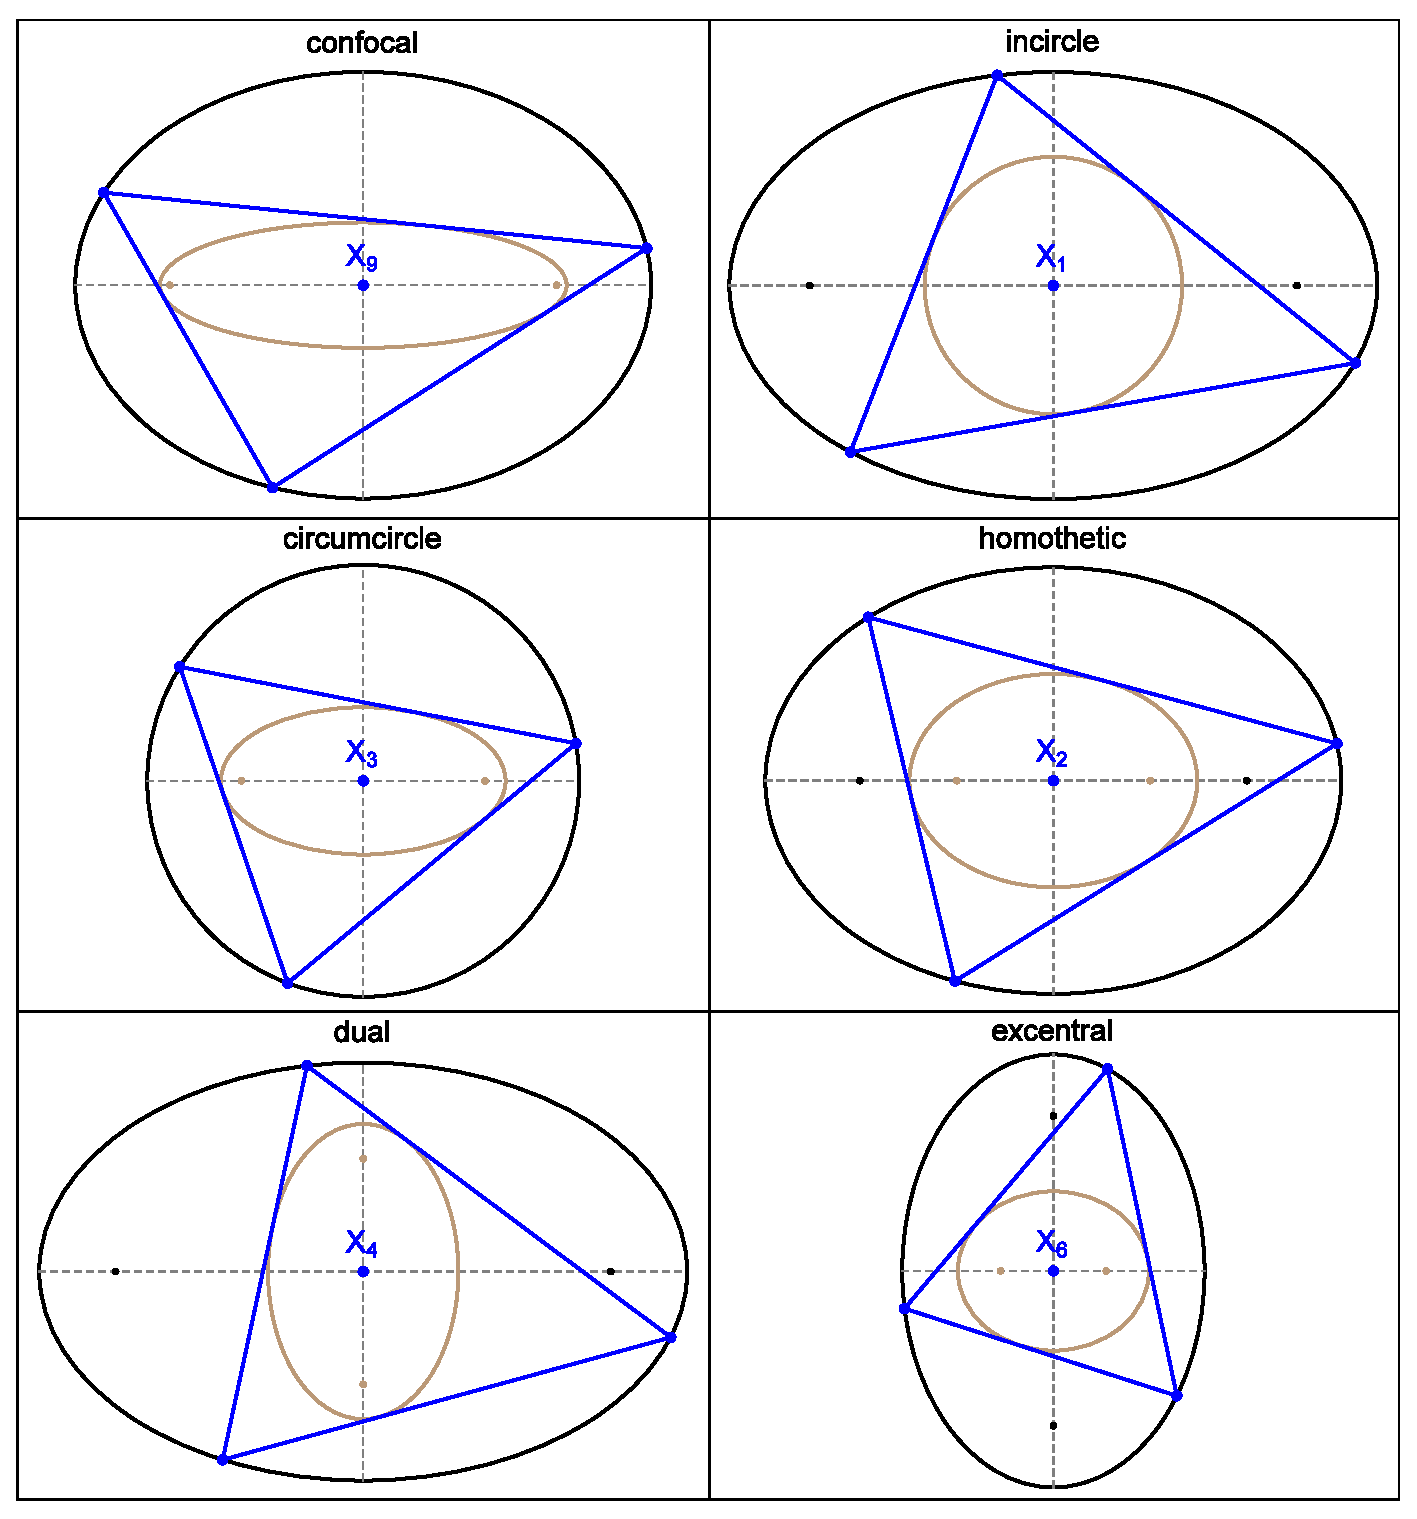
\includegraphics[width=\textwidth]{chap_06/pics/pics_06_015_six_caps_perp}
    \caption{The five concentric, axis-parallel (CAP) families whose loci are studied in this chapter. The confocal family is treated in \cref{chap:05-confocal-loci}. \href{https://youtu.be/14TQ5WlZxUw}{Video}}
    \label{fig:06-six-caps}
\end{figure}

Recall Cayley's condition for a CAP pair to admit a Poncelet 3-periodic family: $a_c/a+b_c/b=1$, where $a>b>0$, $a_c>0$, and $b_c>0$.


\section{Incircle family}

A 3-periodic interscribed in a CAP pair with incircle is shown in \cref{fig:06-six-caps}(top middle).

Recall that for this pair, Cayley implies the inradius $r=\frac{{a}{b}}{a+b}$. Also recall that in \cref{prop:03-n3-incircle-R}, we show that incircle 3-periodics have invariant circumradius $R=(a+b)/2$ and that the locus of the circumcenter $X_3$ is a circle of radius $d=(a-b)/2$ centered on $X_1$, see \cref{fig:03-incircle-circum}.

The next 4 propositions are illustrated in \cref{fig:06-incircle-x2456}.

\begin{figure}
    \centering
    \includegraphics[width=\textwidth]{pics_06_020_incircle_x2456.png}
    \caption{Loci of $X_k$, $k=$2,4,5,6 over incircle 3-periodics. These are ellipses for all but $X_5$ whose locus is a circle. \href{https://bit.ly/2SvuMpi}{Live 1}, \href{https://bit.ly/3fpO098}{Live 2}}
    \label{fig:06-incircle-x2456}
\end{figure}

\begin{proposition}
Over incircle 3-periodics, the locus of the barycenter $X_2$ is an ellipse with axes $a_2=a(a - b)/(3a + 3b)$ and $b_2=b(a - b)/(3a + 3b)$ centered on $O=X_1$.
 \label{prop:06-incircle-X2-locus}
\end{proposition}

\begin{proof}
Follows from \cref{sec:03-cap-vtx-param}.
\end{proof}

\begin{proposition}
Over incircle 3-periodics, the locus of the orthocenter $X_4$ is an ellipse of axes $a_4=(a - b)b/(a + b) $ and $b_4=(a - b)a/(a + b)$
 centered  on $O=X_1$.
\label{prop:06-x4-locus}
\end{proposition}

\begin{proposition}
Over incircle 3-periodics, the locus of the center $X_5$ of the 9-point circle is a circle of radius $d=\frac{(a-b)^2}{4(a+b)}$
  centered on $O=X_1$.
\label{prop:X5}
\end{proposition}

\begin{proof}
Direct, analogous to \cite[Thm.3]{garcia2020-new-properties}.
\end{proof}

\begin{proposition}
Over incircle 3-periodics, the locus of $X_6$ is a quartic given by the following implicit equation:

\begin{align*}
    &   \left( b \left( b+2\,a \right)  \left( {a}^{2}+2\,ab+3\,{b}^{2}
 \right)  {x}^{2}+a \left( a+2\,b \right)  \left( 3\,{a}^{2}+2\,ab+{b}
^{2} \right) {y}^{2} \right) ^{2}\\
&-{a}^{2}{b}^{2} \left( a-b \right) ^{
2} \left( {b}^{2} \left( b+2\,a \right) ^{2}{x}^{2}+{a}^{2} \left( a+2
\,b \right) ^{2}{y}^{2} \right) =0
\end{align*}
\end{proposition}



\section{Circumcircle family}

This family is inscribed in a circle of radius $R$ centered on $O=X_3$ and circumscribes a concentric ellipse with semi-axes $a,b$; see     \cref{fig:06-six-caps}(top right). Recall that the Cayley condition implies $R=a+b$. 

\begin{proposition}
Over circumcircle 3-periodics, the locus of the barycenter $X_2$ is a concentric circle with radius $r_2$ given by:

\[ r_2 = \frac{1}{3}(a-b)  \]

\end{proposition}

Referring to \cref{fig:06-circum-x1456-loci}:

\begin{proposition}
Over circumcircle 3-periodics, the loci of both the orthocenter $X_4$ and the center $X_5$ of the 9-point circle are concentric circles centered on $X_3$, with radii $2 d'$ and $d'$ respectively, where $d'=(a-b)/2$ .
\label{prop:06-circum-x1456-loci}
\end{proposition}

\begin{proof}
Based on 3-periodic vertex parametrization and CAS-assisted algebraic simplification.
\end{proof}

\begin{figure}
    \centering
    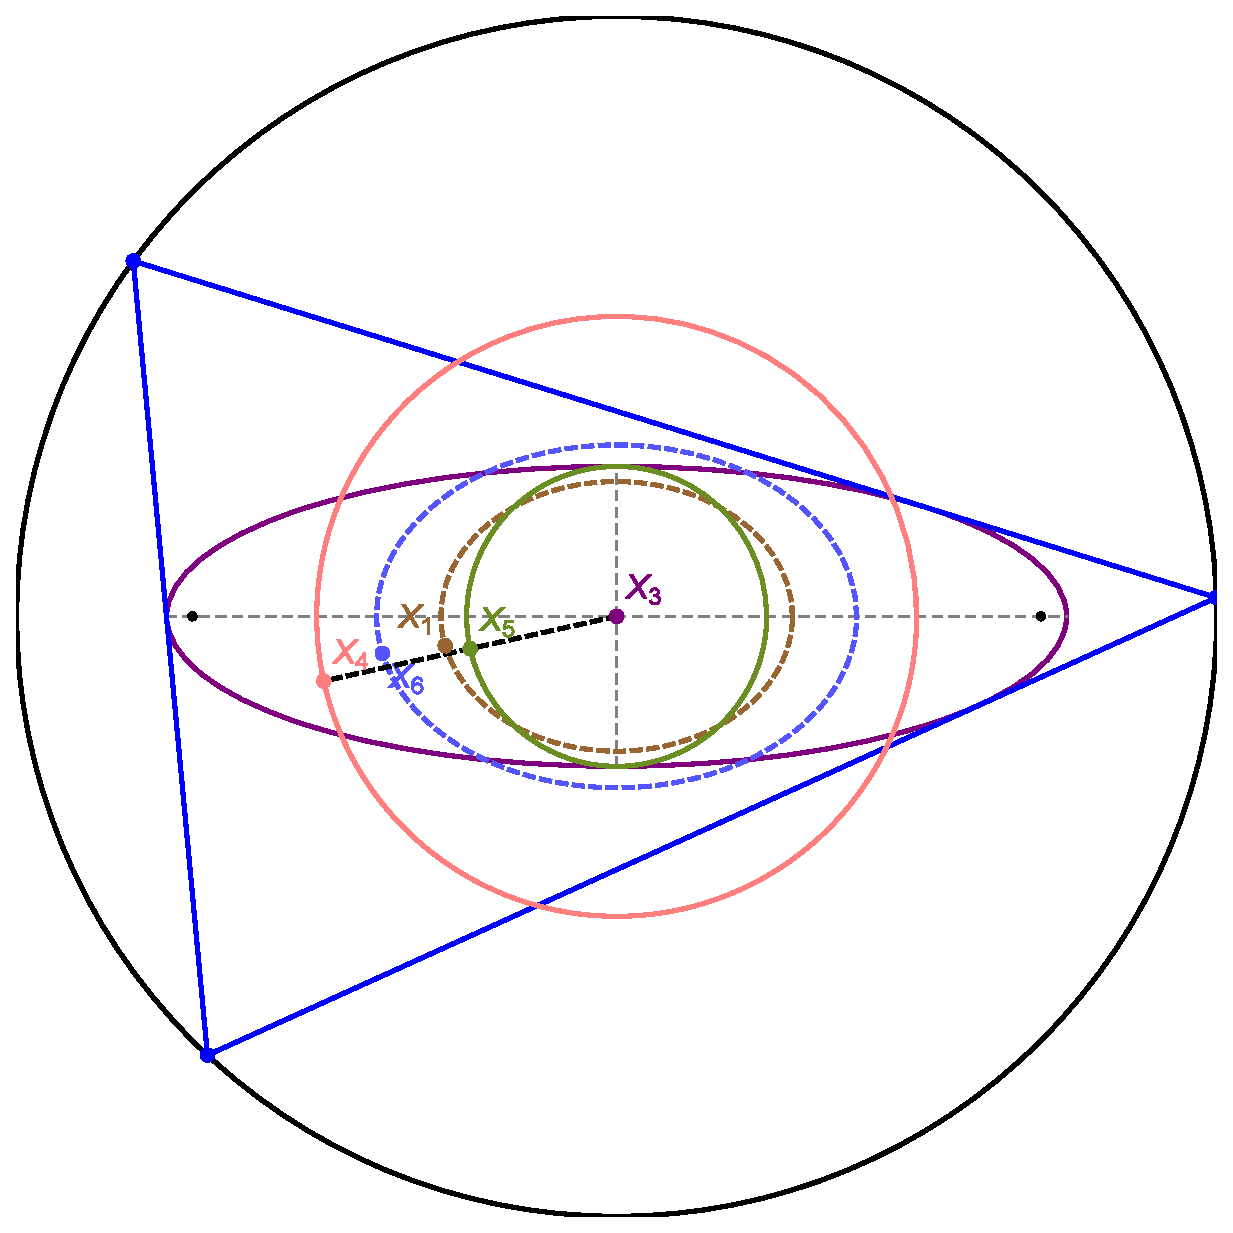
\includegraphics[width=.7\textwidth]{pics_06_030_system_II_locus.eps}
    \caption{A circumcircle 3-periodic: The loci of both orthocenter $X_4$ (pink) and nine-point center $X_5$ (olive green) are concentric with the external circle (black). Their radii are $2d'$ and $d'$, respectively where $d'=|X_4-X_5|$. In contradistinction to the elliptic billiard, the locus of the incenter $X_1$ (dashed brown) is non-elliptic while that of the symmedian point $X_6$ (dashed blue) is an ellipse. \href{https://youtu.be/8xlYaQfQCTw}{Video}, \href{https://bit.ly/3vo8eWl}{Live}}
    \label{fig:06-circum-x1456-loci}
\end{figure}

Recall that in the confocal pair the locus of $X_1$ (resp. $X_6$) is an ellipse (resp. a quartic) \cite{garcia2020-ellipses}; see Appendix~\ref{app:loci-x1x6}. Interestingly:

\begin{proposition}
Over circumcircle 3-periodics, the locus of the symmedian point $X_6$ (resp. the incenter $X_1$) is an ellipse (resp. the convex component of a quartic -- note the other component corresponds to the locus of the 3 excenters which can be concave). These are given by:

\begin{align*}
\text{locus of $X_6$}: &\; \frac{x^2}{a_6^2}+\frac{y^2}{b_6^2}=1, \; a_6=\frac{ a^2 - b^2}{a + 2 b},\;\;  b_6=\frac{ a^2 - b^2}{2a +  b},\\
\text{locus of $X_1$}:&\; \left( {x}^{2}+{y}^{2} \right) ^{2}-2\, \left( a+3\,b \right) 
 \left( a+b \right) {x}^{2}-2\, \left( a+b \right)  \left( 3\,a+b
 \right) {y}^{2} \\
 &+\left( a^2-b^2 \right) ^{2}=0\cdot
 \label{thm:II-loci_X1}
\end{align*}
\end{proposition}

\begin{proof}
CAS-assisted simplification.
\end{proof}


\section{Homothetic family}

The family of 3-periodics interscribed in a pair of homothetic ellipses is depicted in \cref{fig:06-six-caps}(bottom left). Let $a,b$ be the semi-axes of the outer ellipse. The Cayley condition for this pair implies that $a_c=a/2$ and $b_c=b/2$, see  \cref{prop:03-homothetic-cayley}.

Recall the barycenter $X_2$ is stationary at the common center and the area $A=(3 a b \sqrt{3})/{4}$ is invariant.

Recall that over the confocal family, the locus of the incenter $X_1$ (resp. symmedian point $X_6$) was an ellipse (resp. a quartic). Teferring to \cref{fig:06-homoth-x1x6}, this is reversed in the homothetic family: 

\begin{proposition}
Over homothetic 3-periodics, the locus of the incenter $X_1$ (resp. symmedian point $X_6)$ is a quartic (resp. an ellipse). These are given by:

\begin{align*}
\text{locus of $X_1$}: \;& 
16\, \left( {a}^{2}{y}^{2}+{b}^{2}{x}^{2} \right)  \left( {a}^{2}{x}^{
2}+{b}^{2}{y}^{2} \right) -8\,{b}^{2} \left( {a}^{4}+5\,{a}^{2}{b}^{2}
+2\,{b}^{4} \right) {x}^{2}\\
&-8\,{a}^{2} \left( 2\,{a}^{4}+5\,{a}^{2}{b}
^{2}+{b}^{4} \right) {y}^{2}+{a}^{2}{b}^{2} \left( a^2-b^2 \right) ^{2}=0,
 \\
\text{locus of $X_6$}: &\; \frac{x^2}{a_6^2}+\frac{y^2}{b_6^2}=1,\;a_6=\frac{a(a^2-b^2)}{2(a^2+b^2)},\;\;\; b_6=\frac{b(a^2-b^2)}{2(a^2+b^2)} \cdot\\
\end{align*}
\label{prop:06-homoth-x1x6}
\end{proposition}

\begin{figure}
    \centering
    \includegraphics[width=.7\textwidth]{chap_06/pics/pics_06_040_homoth_x16.png}
    \caption{A homothetic 3-periodic and the quartic (resp. elliptic) locus of the incenter $X_1$ (resp. symmedian point $X_6$). \href{https://bit.ly/3oR5nCN}{Live}}
    \label{fig:06-homoth-x1x6}
\end{figure}

\begin{proof}
CAS-assisted simplification.
\end{proof}

\subsection{Four Circular Loci}

The two Fermat points $X_{13}$ and $X_{14}$ as well as the two isodynamic points $X_{15}$ and $X_{16}$ have trilinear coordinates which are irrational on the sidelengths of a triangle, see \cite{etc}. Indeed, over billiard 3-periodics, their loci are non-elliptic.

Referring to \cref{fig:06-homoth-circ-loci}:

\begin{proposition}
Over homothetic 3-periodics, the loci of $X_k$, $k=$13,14,15,16 are four distinct circles. Their radii are $(a-b)/2$, $(a+b)/2$, $(a-b)^2/z$, and $(a+b)^2/z$, respectively, where $z=2(a+b)$.
\label{prop:06-homoth-four-circles}
\end{proposition}

\begin{figure}
    \centering
    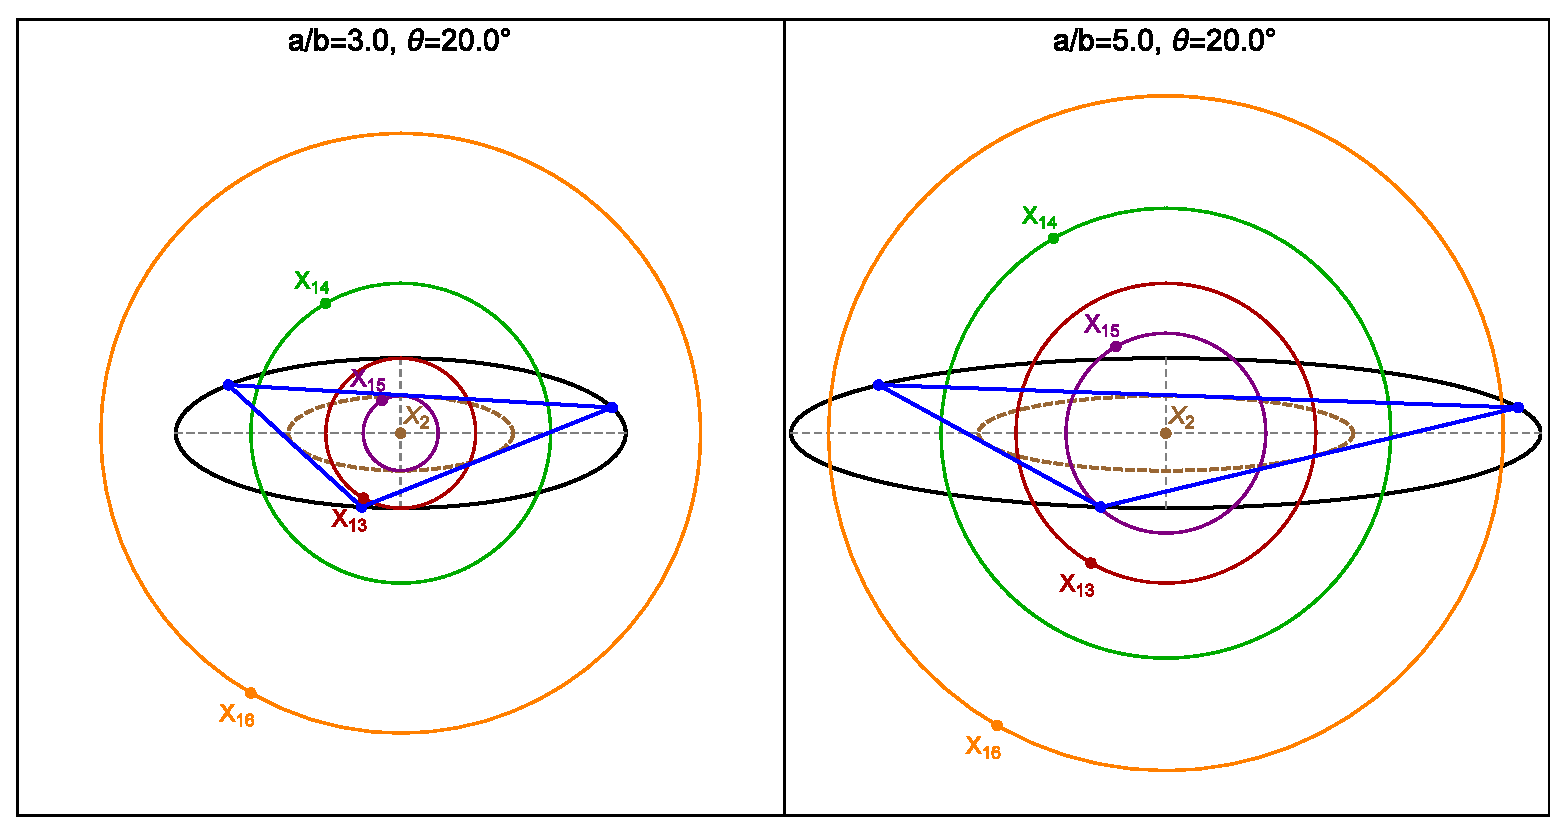
\includegraphics[width=\textwidth]{pics_06_050_system_III_circular_loci.eps}
    \caption{Circular loci of the first and second Fermat points $X_{13}$ and $X_{14}$ (red and green) as well as the first and second isodynamic points $X_{15}$ and $X_{16}$ (purple and orange) for two aspect ratios of the homothetic pair: $a/b=3$ (left) and $a/b=5$ (right). The radius of the $X_{16}$ locus is minimal at the first case. \href{https://youtu.be/ZwTfwaJJitE}{Video}, \href{https://bit.ly/3yF0wc9}{Live}}
    \label{fig:06-homoth-circ-loci}
\end{figure}
\subsection{Loci of the Brocard points}

\begin{figure}
    \centering
\includegraphics[width=\textwidth]{pics_06_060_first_brocard_tri_locus.eps}
\caption{Over homothetic 3-periodics, the loci of the two Brocard points $\Omega_1$ and $\Omega_2$ are tilted ellipses (red and green) of aspect ratio equal to those in the pair, see \href{https://youtu.be/2fvGd8wioZY}{Video}. Also shown (dashed orange) is the locus of the vertices of the first Brocard triangle (orange): this is an axis-aligned ellipse also homothetic to the pair.\href{https://youtu.be/13i3JGY-fK4}{Video}, \href{https://bit.ly/3iaISog}{Live}}
\label{fig:06-homot-loci}
\end{figure}

Referring to Figure~\ref{fig:06-homot-loci}:

\begin{proposition}
Over homothetic 3-periodics, the loci of the Brocard points $\Omega_1$ and $\Omega_2$ are ellipses $\E_1$ and $\E_2$ which modulo rotation are homothetic to the ellipses in the pair. The loci are reflected images of each other about either the $x$ or $y$ axis.
\end{proposition}

\begin{proof}
The loci are given by
	
	\[\E_1(x,y)= {\frac { \left( 7\,{a}^{4}+6\,{a}^{2}{b}^{2}+3\,{b}^{4} \right) {x}^{2
}}{{a}^{2} \left( a^2-b^2 \right) ^{2}   }}+{\frac {
 \left( 3\,{a}^{4}+6\,{a}^{2}{b}^{2}+7\,{b}^{4} \right) {y}^{2}}{{b}^{
2} \left( {a}^{2}-  {b}^{2} \right)^2 }}- \,{\frac {
4\sqrt {3} \left( {a}^{2}+{b}^{2} \right) xy}{ab \left( {a}^{2}-{b}^{2}
 \right) }}-1
	\]
	\[\E_2(x,y)=	 {\frac { \left( 7\,{a}^{4}+6\,{a}^{2}{b}^{2}+3\,{b}^{4} \right) {x}^{2
}}{{a}^{2} \left( a^2-b^2 \right) ^{2}   }}+{\frac {
 \left( 3\,{a}^{4}+6\,{a}^{2}{b}^{2}+7\,{b}^{4} \right) {y}^{2}}{{b}^{
2} \left( {a}^{2}- {b}^{2} \right)^2 }}+ \,{\frac {
4\sqrt {3} \left( {a}^{2}+{b}^{2} \right) xy}{ab \left( {a}^{2}-{b}^{2}
 \right) }}-1
\]	
	The angle $\theta$ between the axes of ellipses $\E_1$  and $\E_2$ is given by
	\[\tan\theta = \frac{4\sqrt{3}(a^2+b^2) ab}{3a^4+2a^2b^2+3b^4}.\]
\end{proof}

In no other CAP family so far studied, is the locus of either Brocard point an ellipse. This informs:

\begin{conjecture}
Over 3-periodics in a CAP family, the locus of the Brocard points is an ellipse if and only if the ellipses are homothetic.
\label{conj:06-homoth-broc-loci}
\end{conjecture}


\subsection{First Brocard triangle: vertex locus}

Consider a triangle $T=P_1 P_2  P_3 $ with Brocard points $\Omega_1$ and $\Omega_2$. Referring to Figure~\ref{fig:06-first-broc-tri}:

\begin{definition}[First Brocard Triangle]
The vertices $P_1'$, $P_2'$, $P_3'$ of the First Brocard Triangle $T_1$ are defined as follows: $P_1'$ (resp. $P_2'$, $P_3'$) is the intersection of $P_2{\Omega_1}$ (resp. $P_3{\Omega_1}$, $P_1{\Omega_1}$) with $P_3{\Omega_2}$ (resp. $P_1{\Omega_2}$, $P_2{\Omega_2}$).
\end{definition}

Know properties of the $T_1$ include that (i) it is inversely similar to $T$, (ii) its barycenter $X_2$ coincides with that of the reference triangle, and (iii) its vertices are concyclic with $\Omega_1$, $\Omega_2$, $X_3$, and $X_6$ on the Brocard circle \cite[Brocard Circle]{mw}, whose center is $X_{182}$. Referring to Figure~\ref{fig:06-homot-loci}:

\begin{figure}
    \centering
    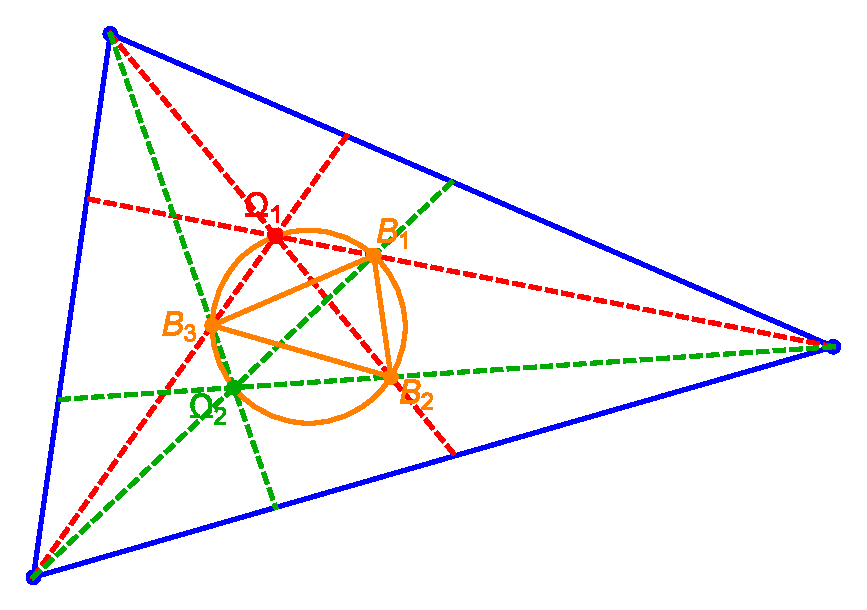
\includegraphics[width=.7\textwidth]{pics_06_070_first_brocard_tri}
    \caption{Construction for the First Brocard Triangle (orange) taken from \cite[First Brocard Triangle]{mw}. It is inversely similar to the reference one (blue), and their barycenters $X_2$ are common. Its vertices $B_1,B_2,B_3$ are concyclic with the Brocard points $\Omega_1$ and $\Omega_2$ on the Brocard circle (orange).}
    \label{fig:06-first-broc-tri}
\end{figure}

\begin{proposition}
Over 3-periodics in the homothetic pair, the locus of the vertices of $T_1$ is an axis-aligned, concentric ellipse, homothetic to the ones in the pair and interior to the caustic. Its axes are given by: 
\[ a'=\frac{a(a^2-b^2)}{2(a^2+b^2)},\;\;\; b'=\frac{b(a^2-b^2)}{2(a^2+b^2)}\]
\end{proposition}

\begin{proof}
The locus must be an ellipse since $T_1$ is inversely similar to the 3-periodics whose vertices are inscribed in an ellipse and their barycenters coincide. A vertex of the Brocard triangle is parametrized by

\[ \frac{x^2}{a'^2}+\frac{y^2}{b'^2} = 1 \]
\end{proof}

Since homothetic 3-periodics conserve area \cite{reznik2020-similarityII}, so must $T_1$ (inversely similar). Its area can be computed explicitly:

\begin{proposition}
Over 3-periodics in the homothetic pair, the area of $T_1$ is invariant and given by
\[ {\frac {3\sqrt{3} ab\left( {a}^{2}-{b}^{2} \right) ^{2}  }{16
 \left( {a}^{2}+{b}^{2} \right) ^{2}}}
\]
\end{proposition}






\subsection{Loci of Fermat and Isodynamic Equilaterals}

As seen in \cref{sec:04-brocard-isodyn-pedals}, the pedal triangles from either the Fermat $X_{13},X_{14}$ and Isodynamic $X_{15},X_{16}$ points are equilateral. Since the homothetic family conserves $\Sha=\cot\omega$, \cref{prop:04-equi-areas} implies:

\begin{corollary}
Over homothetic 3-periodics, the areas $A_k$, $k=13,14,15,16$ of the equilateral pedals from the Fermat and Isodynamic points are invariant.
\label{cor:06-equi-areas}
\end{corollary}

Over the Brocard porism, the loci of said equilaterals, were shown to be circles, see \cref{fig:04-isodynamic-equis}. Interestingly, and referring to \cref{fig:06-homot-equis}:

\begin{figure}
    \centering
    \includegraphics[width=\textwidth]{pics_06_090_homot_isos.eps}
    \caption{The homothetic Poncelet family (stationary $X_2$) is equibrocardal (conserves $\omega$) and its triangles (blue) have invariant area. The loci of $X_k,k=13,14,15,16$ are circles concentric with the ellipses \href{https://youtu.be/ZwTfwaJJitE}{Video}. Since areas $A_{15}$, $A_{16}$, $A_{13}$, $A_{14}$ only depend on $\cot\omega$, they are individually invariant. The loci of $X_{396}$ and $X_{395}$ are ellipses whereas those of $X_{5463}$ and $X_{5464}$ are circles.
    \href{https://youtu.be/7qoxAaG8sbk}{Video}}
    \label{fig:06-homot-equis}
\end{figure}
\section{Dual Family}

The dual family (bottom middle in \cref{fig:06-six-caps}) is interscribed between two CAP ellipses with reciprocal aspect ratios. Its orthocenter $X_4$ is stationary. Referring to \cref{fig:06-dual-x2345}:

\begin{proposition}
Over dual 3-periodics, the loci of $X_2$, $X_3$, and $X_5$ are ellipses.
\label{prop:06-dual-x2345}
\end{proposition}

\begin{figure}
    \centering
    \includegraphics[width=.7\textwidth]{pics_06_100_dual_x2345.png}
    \caption{Over dual 3-periodics (stationary $X_4$), the loci of $X_2$, $X_3$, and $X_5$ are ellipses. \href{https://bit.ly/3wE3zQg}{Live}}
    \label{fig:06-dual-x2345}
\end{figure}

\section{Excentral Family}

Recall in \cref{thm:02-incenter-excenter}, we derived the semi-axes of the locus of the excenters, i.e., the ellipse in which the excentral family is inscribed. 

Also recall \cref{sec:05-golden-locus} where it was noted that over the excentral family, the locus its circumcenter ($X_{40}$ in terms of billiard 3-periodics) was identical to a rotated copy of caustic (i.e., the elliptic billiard) when the latter's aspect ratio is $\varphi$ the golden ratio.

Referring to \cref{fig:06-excentral-loci}:

\begin{proposition}
Over excentral 3-periodics the locus of $X_2$, $X_3$ and $X_4$ are ellipses.
\label{prop:06-excentral-loci}
\end{proposition}

\begin{figure}
    \centering
    \includegraphics[width=\textwidth]{pics_06_110_excentral_loci.png}
    \caption{Elliptic loci of $X_k$, $k=$2,3,4 over excentral 3-periodics (the symmedian $X_6$ is stationary at the center). \href{https://bit.ly/2RSwAZF}{Live}}
    \label{fig:06-excentral-loci}
\end{figure}

\section{Summary}

\cref{tab:04-xn-comparison} summarizes the types of loci (point, circle, ellipse, etc.) for some triangle centers for families analyzed in this and previous chapters (including non-concentric such as poristic triangles and Brocard's porism). Families are grouped according to similar patterns in their loci types.

\begin{table}
\small
\centering
\begin{tabular}{|c||c|c|c||c|c|c||c|c||}
\hline
& \multicolumn{3}{c||}{Group A} & \multicolumn{3}{c||}{Group B} & \multicolumn{2}{c||}{Group C} \\
\hline
 & Conf. & Inc. & Por. & Exc. & Circ. &  \makecell{Por.\\Exc.} & Hom. & Broc. \\
 \hline
$X_1$ & E & P & P & X&X & X & 4 & X \\
$X_2$ & E & E & C & E&C & P & P & C \\
$X_3$ & E & C & P & E&P & P & E & P \\
$X_4$ & E & E & C & E&C & P & E & C \\
$X_5$ & E & C & C & E&C & P & E & C \\
$X_6$ & 4 & 4 & \textcolor{red}{\textbf{E}} & P&E & C & E & P \\
$X_7$ & E & E & C & X & X & X & X & X \\
$X_8$ & E & E & C & X & X & X & X & X \\
$X_9$ & P & E & C & X & X & X & X & X \\
$X_{10}$ & E & E & C & X & X & X & X & X \\
$X_{11}$ & E$''$ & C$''$ & C$''$ & X & X & \textcolor{red}{\textbf{C$_5$}} & X & X \\
$X_{12}$ & E & C & C & X & X & X & X & X \\
$X_{13}$ & X & X & X & X & X & X & C & C \\
$X_{14}$ & X & X & X & X & X & X & C & C \\
$X_{15}$ & X & X & X & X & X & X & C & P \\
$X_{16}$ & X & X & X & X & X & X & C & P \\
$X_{99}$ & X & X & C$'$ & \textcolor{red}{\textbf{X}}&C$'$ & C$'$ & E$'$ & C$'$ \\
$X_{100}$ & E$'$ & E$'$ & C$'$ & \textcolor{red}{\textbf{X}}&C$'$ & C$'$ & \textcolor{red}{\textbf{X}} & C$'$ \\
$X_{110}$ & X & X & C$'$ & E$'$&C$'$ & C$'$ & \textbf{X} & C$'$ \\
 \hline
\end{tabular}
\caption{Loci types (P, C, E, X indicate point, circle, ellipse, and non-elliptic (degree not yet derived) loci, respectively) of some triangle centers over 3-periodic families. These are clustered in in 3 groups A,B,C sharing many metric phenomena: (i) confocal, incircle, poristic; (ii) excentral, circumcircle, poristic-excentral; (iii) homothetic and Brocard porism. A numeric entry indicates the degree of the non-elliptic implicit, e.g., '4' for quartic. A singly (resp. doubly) primed letter indicates a perfect match with the outer (resp. inner) conic in the pair. The symbol C$_5$ refers to the nine-point circle. The boldface entries indicate a discrepancy in the cluster. Note: $X_n$ for the confocal and poristic excentral triangles refer to triangle centers of the family itself (not of their reference triangles).}
\label{tab:04-xn-comparison}
\end{table}

The first row reveals that out of the 8 families considered only in the confocal case is the locus of the incenter $X_1$ an ellipse, suggesting this is a rare phenomenon.

The plethora of circles in the poristic family had already been shown in \cite{odehnal2011-poristic}. A significant occurrence of ellipses in the confocal pair was signalled in \cite{garcia2020-ellipses}. As mentioned above, irrational centers $X_k$, $k\in[13,16]$ sweep out circles for the homothetic pair. $X_{15}$ and $X_{16}$ are known to be stationary over the Brocard family \cite{bradley2007-brocard}, however the locus of $X_{13}$ and $X_{14}$ are circles. Also noticeable is the fact that (i) though in the confocal pair the locus of $X_1$ (resp. $X_6$) is an ellipse (resp. quartic), locus types are swapped for both circumcircle and homothetic families.

It is well-known that there is a projective transformation that takes any Poncelet family to the the confocal pair,  \cite{dragovic11}. In this case only projective properties are preserved.

As mentioned above, the confocal family is the affine image of either the incircle or circumcircle family. In the first (resp. second) case the caustic (resp. outer ellipse) is sent to a circle. Though the affine group is non-conformal, we showed above that both families conserve the sum of cosines. One way to see this is that there is an alternate, conformal path which takes incircle 3-periodics to confocal ones, namely through a rigid rotation (yielding poristic triangles), followed by a variable similarity (yielding the confocal family).

A similar argument is valid for circumcircle triangles: there is an affine path (non-conformal) to the confocal family though both conserve the product of cosines. Notice there is also an alternate conformal composition of rotation (yielding poristic excentral triangles) and a variable similarity (yielding confocal excentral triangles). All in this path conserve the product of cosines.

Finally, homothetic and Brocard porism 3-periodics form an isolated clique. As mentioned in \cite{reznik2020-similarityII}, these are variable similarity images of one another but cannot be mappable to the other families via similarities nor affinely.

\subsection{Loci Types, CAP families}
\label{sec:06-loci-types}

Below we list triangle centers such that their loci types are either points or conics. These are obtained via numerical simulation amongst the first 200 centers in \cite{etc}.

\begin{itemize}
    \item Confocal (stationary $X_9$)
    \begin{itemize}
	\item Circles (0): n/a
	\item Ellipses (42): 1, 2, 3, 4, 5, 7, 8, 10, 11, 12, 20, 21, 35, 36, 40, 46, 55, 56, 57, 63, 65, 72, 78, 79, 80, 84, 88, 90, 100, 104, 119, 140, 142, 144, 145, 149, 153, 162, 165, 190, 191, 200. Note: the first 29 in the list were proved in \cite{garcia2020-ellipses}
	\end{itemize}
    \item Incircle: (stationary $X_1$)
    \begin{itemize}
    \item Circles (15): 3, 5, 11, 12, 35, 36, 40, 46, 55, 56, 57, 65, 80, 119, 165.
    \item Ellipses (26): 2, 4, 7, 8, 9, 10, 20, 21, 63, 72, 78, 79, 84, 90, 100, 104, 140, 142, 144, 145, 149, 153, 170, 176, 191, 200.
    \end{itemize}
    \item Circumcircle: (stationary $X_3$)
	\begin{itemize}
	\item Circles (28): 2, 4, 5, 20, 22, 23, 24, 25, 26, 74, 98, 99, 100, 101, 102, 103, 104, 105, 106, 107, 108, 109, 110, 111, 112, 140, 156, 186, 201.
	\item Ellipses (34): 6, 15, 21, 27, 28, 39, 49, 51, 52, 54, 58, 61, 64, 66, 67, 68, 69, 70, 113, 125, 141, 143, 146, 154, 155,  159, 161, 182, 184, 185, 193, 195, 199.
	\end{itemize}
    \item Homothetic: (stationary $X_2$)
	\begin{itemize}
    \item Circles (4): 13, 14, 15, 16.
	\item Ellipses (29): 3, 4, 5, 6, 17, 18, 20, 32, 39, 61, 62, 69, 76, 83, 98, 99, 114, 115, 140, 141, 147, 148, 182, 187, 190, 193, 194.
	\end{itemize}
	\item Dual: (stationary: $X_4$)
	\begin{itemize}
    \item Circles (0): n/a
    \item Ellipses (10): 2, 3, 5, 20, 64, 107, 122, 133, 140, 154.
    \end{itemize}
	\item Excentral: (stationary: $X_6$)
	\begin{itemize}
    \item Circles (0): n/a
    \item Ellipses (39): 2, 3, 4, 5, 20, 22, 23, 24, 25, 26, 49, 51, 52, 54, 64, 66, 67, 68, 69, 70, 74, 110, 113, 125, 140, 141, 143, 146, 154, 155, 156, 159, 161, 182, 184, 185, 186, 193, 195.

    \end{itemize}
\end{itemize}

Semi-axes lengths for the elliptic loci of many triangle centers are available in \cite{garcia2021-ellipses-web}.

\subsection{Loci Types, NCAP Families}
\label{sec:06-ncap-loci}

For completeness, included below are point and/or conic loci for both Poristic and Brocard triangles. These include many stationary centers as well as segment and hyperbolic loci. 

\begin{itemize}
\item Poristic, see \cite{odehnal2011-poristic}
    \begin{itemize}
    \item Points (11): 1, 3, 35, 36, 40, 46, 55, 56, 57, 65, 165. 
    \item Segments (2): 44, 171.
    \item Circles (46): 2, 4, 5, 7, 8, 9, 10, 11, 12, 20, 21, 23, 63, 72, 74, 78, 79, 80, 84, 90, 98, 99, 100, 101, 102, 103, 104, 105, 106, 107, 108, 109, 110, 111, 112, 119, 140, 142, 143, 144, 145, 149, 153, 186, 191, 200.
	\item Ellipses (39): 6, 19, 22, 24, 25, 28, 31, 33, 34, 37, 38, 41, 42, 43, 45, 47, 48, 51, 52, 54, 58, 59, 60, 71, 73, 77, 81, 88, 89, 169, 170, 181, 182, 184, 185, 195, 197, 198, 199.
	\item Hyperbolas (7): 26, 49, 64, 154, 155, 156, 196.
	\end{itemize}
\item{Brocard porism}
    \begin{itemize}
    \item Points (10): 3, 6, 15, 16, 32, 39, 61, 62, 182, 187.
    \item Segments (3): 50, 52, 58.
	\item Circles (38): 2, 4, 5, 13, 14, 17, 18, 20, 23, 69, 74, 76, 83, 98, 99, 100, 101, 102, 103, 104, 105, 106, 107, 108, 109, 110, 111, 112, 114, 115, 140, 141, 147, 148, 183, 186, 193, 194.
	\item Ellipses (6): 24, 25, 51, 143, 157, 18.
	\item Hyperbolas (5): 26, 49, 64, 154, 159.
	\end{itemize}
\end{itemize}



\section{Exercises}

\begin{exercise}
Prove that over incircle 3-periodics, the power of the center with respect to the (fixed radius) circumcircle is invariant and  equal to $-a b$.
\end{exercise}

\begin{exercise}
Compute $a/b$ of the external ellipse in the incircle CAP family such that (i) the circular locus of $X_3$ coincides with the incircle, (ii) the elliptic locus of $X_4$ touches the outer ellipse at its top and bottom vertices, and (iii) the circular locus of $X_5$ coincides with the incircle. See it \href{https://bit.ly/3wzw1CD}{Live1}, \href{https://bit.ly/3vnVHlL}{Live2}.
\end{exercise}

\begin{exercise}
Derive the radius of the circumcircle in the same-named family such that the quartic locus of $X_1$ and the circular locus of $X_4$ intersect at four points on the inner ellipse, see it \href{https://bit.ly/3wzQkjp}{Live}. 
\end{exercise}

\begin{exercise}
Prove \cref{prop:06-homoth-four-circles}.
\end{exercise}

\begin{exercise}
Prove that over homothetic 3-periodics, the radius of the circular locus of $X_{16}$ is minimum when $a/b=3$.
\end{exercise}

\begin{exercise}
Prove that at $a/b=\sqrt{5}$, the elliptic loci of the Brocard points over homothetic 3-periodics are internally tangent to the inner ellipse.  See it \href{https://bit.ly/3fkEMuG}{Live}.
\end{exercise}

\begin{exercise}
Derive the $a/b$ such that the elliptic loci of the Brocard points over the homothetic family intersect the y axis at $b/2$, i.e., at the top vertex of the caustic. See it \href{https://bit.ly/3fm8G1u}{Live}.
\end{exercise}

\begin{exercise}
Prove that over homothetic 3-periodics, the locus of the Brocard midpoint $X_{39}$ is an ellipse, derive its axis.
\end{exercise}

\begin{exercise}
Show that over homothetic 3-periodics, the elliptic locus of the vertices of the first Brocard triangle is interior to the inner ellipse.
\end{exercise}

\begin{exercise}
Compute the invariant similarity ratio of homothetic 3-periodics to the first Brocard triangles. 
\end{exercise}

\begin{exercise}
Derive expressions for the areas in \cref{cor:06-equi-areas}.
\end{exercise}

\begin{exercise}
Synthesize a triangle center such that over billiard 3-periodics its locus is a circle? Hint: it will be an affine combination of $X_2$ and $X_3$.
\end{exercise}

\begin{exercise}
Derive semi-axes for the dual family elliptic loci of $X_2$, $X_3$, and $X_5$ in \cref{prop:06-dual-x2345}.
\end{exercise}

\begin{exercise}
As shown in \cref{sec:06-ncap-loci}, over poristic triangles, the locus of $X_{44}$, and $X_{171}$ are segments. Derive their data. Do the same for the segment-loci of $X_{50}$, $X_{52}$, $X_{58}$ over Brocard porism 3-periodics.
\end{exercise}

\begin{exercise}
Given an ellipse $\E$ with semi-axes $a$, $b$, consider a non-Ponceletian family of triangles with two vertices fixed on the foci of $\E$ and a third one which sweeps the boundary. Show the locus of the incenter of this family is an ellipse. See it \href{https://bit.ly/3up4a6V}{Live}.
\end{exercise}

\begin{exercise}
Prove that over the Brocard porism, the locus of $X_{114}$ is a circle concentric with, and exterior to, the Brocard inellipse. Derive its radius. \href{https://bit.ly/3g6pmcv}{Live}
\end{exercise}

\begin{exercise}
Prove that over the Brocard porism, the locus of $X_{115}$ is a circle concentric with the Brocard inellipse of radius equal to the latter's minor semi-axis. \href{https://bit.ly/3pfR5Mc}{Live}
\end{exercise}

\begin{exercise}
Over the Brocard porism, the locus of $X_{185}$ is an ellipse which intersects the major axis of the Brocard inellipse $\E'$ in two points $A$ and $B$, see it \href{https://bit.ly/2Rn0chC}{Live}. In the $1<a/b<2$ range, $A,B$ appear to lie between the foci of $\E'$, however for larger $a/b$, e.g., $a/b=3$, the locus seems to pass through the foci, see it \href{https://bit.ly/3icu7Eh}{Live}. Prove or disprove this statement. Derive the center and semi-axes of the locus. 
\end{exercise}
\section{Research Questions}

\begin{question}
Prove (or disprove) \cref{conj:06-homoth-broc-loci}.
\end{question}

\begin{question}
Prove that over homothetic 3-periodics, the locus of center $X_{5463}$ (resp. $X_{5464}$) of the first (resp. second) isogonic equilateral antipedal coincides with the circular locus of $X_{13}$ (resp. $X_{14}$).
\end{question}

\begin{question}
Prove that over homothetic 3-periodics, the locus of the centers $X_{396}$ (resp. $X_{395}$) of the isodynamic equilateral pedals are two ellipses, and derive their semi-axes.
\end{question}

\begin{question}
Can a triangle center be found such that over excentral (or dual) 3-periodics its locus is a circle? 
\end{question}

\begin{question}
Show that over the poristic family (see \cref{sec:04-poristic}), the locus of $X_{59}$ is an ellipse whose major vertices are internally tangent to the outer circle poristics are inscribed in. See it \href{https://bit.ly/2R5laS4}{Live}.
\end{question}

\begin{question}
Prove \cref{prop:06-excentral-loci} and derive the semi-axes of the elliptic loci of the named centers.
\end{question}

\chapter[Homothetic and Brocard Invariants]{Invariants of the Homothetic and Brocard Families}
\label{chap:07-homoth}
%In the previous chapter we restricted ourselves to observing various interesting locus-related phenomena in the confocal pair. 
Namely, we attempt to answer the following related questions:

\begin{itemize}
    \item When are loci algebraic?
    \item What is the type of curve for the locus of the incenter (and excenters) in a generic concentric, axis-parallel (CAP) pair?
    \item In \cite{sergei2016-com} it is shown that over Poncelet N-periodics in a generic pair of conics, the locus of vertex and area centroids is an ellipse. For triangles, both points collapse to $X_2$. Given 3-periodics in a generic pair of ellipses, when is the locus of some triangle center an ellipse? To answer we will use technique based on Blaschke products \cite{daepp-2019}, review below;
    \item We consider the special case of 3-periodics in a pair with a circumcircle, showing that many such loci are circles.
\end{itemize}
\input{chap_07/07_020_algebraic_loci}
\section{Review: Blaschke Products}
\label{sec:07-blaschke}

As a tool for further results in this chapter, we will use a special parametrization of Poncelet 3-periodics based on {em Blaschke Products}, described in \cite{daepp-2019}, used by us in  \cite{helman2021-power-loci}.

Here we consider 3-periodics inscribed in a unit circle and circumscribing a non-concentric ellipse. We will work in the complex plane. Under the Blaschke parametrization, Poncelet 3-periodic vertices become symmetric with respect to the information of the circle-ellipse pair.

\begin{figure}
    \centering
    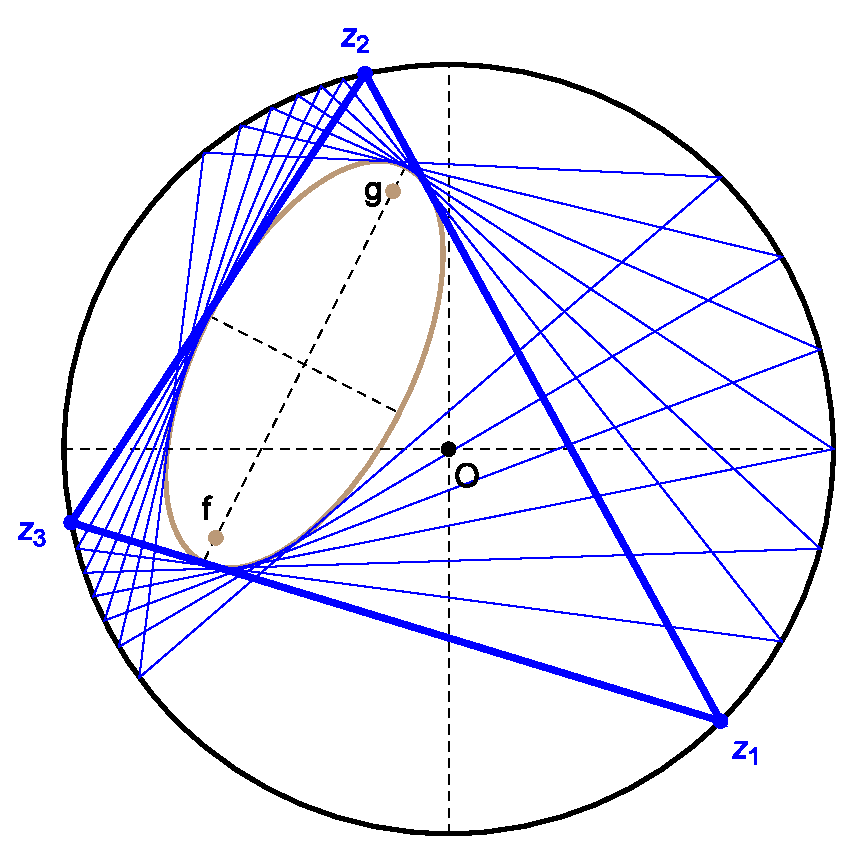
\includegraphics[width=.7\textwidth]{pics_07_050_blaschke_circum}
    \caption{Blaschke complex parametrization of Poncelet 3-periodics (blue). Vertices are $z_1,z_2,z_3$. The foci of the caustic are $f,g$. }
    \label{fig:07-blaschke}
\end{figure}

%As a first step, identify points in $\R^2$ with points in the complex plane $\Cp$. Let $\D$ denote the open unit disk $\{z\in\Cp : |z|<1\}$ and $\T$ denote the unit circle $\{z\in\Cp : |z|=1\}$. By translation and scaling, we may assume the outer circle of the pair to be the unit circle $\T$. Let $\{f,g\}$ be the two foci of the inner ellipse.

Let  $\mathbb{T } = \{ z\in \mathbb{C}: |z| = 1\} $ the unit circle and $\mathbb{D} = \{ z\in\mathbb{C} : |z| < 1\} $ the open unit disk
bounded by $\mathbb{T }.$

Referring to \cref{fig:07-blaschke}, let $z_1,z_2,z_3\in\Cp$ denote the vertices of Poncelet 3-periodics in a generic $N=3$ family with fixed (unit) circumcircle denoted $\T=\{z\in\Cp : |z|=1\}$. Let $f,g$ be the foci of the caustic. Using Viète's formula, we obtain the following parametrization of the elementary symmetric polynomials on $z_1,z_2,z_3$ \cite{daepp-2019}:

\begin{definition}[Blaschke's Parametrization]
\begin{align*}
    \sigma_1:=z_1+z_2+z_3=& f+g+\l\ol f \ol g \\
    \sigma_2:=z_1 z_2+z_2 z_3+z_3 z_1=& f g+\l(\ol f+\ol g) \\
    \sigma_3:=z_1 z_2 z_3=& \l
\end{align*}
where $\l\in\T$ is the varying parameter.
\label{def:bla}
\end{definition}

\noindent Note that the concentric case occurs when $g=-f$.

For each $\l\in\T$, the three solutions of $B(z)=\l$ are the vertices of a 3-periodic orbit of the Poncelet family of triangles in the complex plane, \cite[Chapter 4]{daepp-2019}. Furthermore, as $\l$ varies in $\T$, the whole family of triangles is covered. Clearing the denominator in this equation and passing everything to the left-hand side, we get

\[
z^3-(f+g+\l\ol{f} \ol{g})z^2+(f g+\l(\ol f+\ol g))z-\l=0
\]

\begin{lemma}
If $u,v,w\in\mathbb{C}$ and $\lambda$ is a parameter that varies over the unit circle $\T\subset\mathbb{C}$, then the curve parametrized by
\[ F(\lambda)=u \lambda+ \frac{v}{\lambda}+w \]
is an ellipse centered at $w$, with semiaxis $|u|+|v|$ and $\big||u|-|v|\big|$, rotated with respect to the horizontal axis of $\mathbb{C}$ by an angle of $(\arg u+\arg v)/2$.
\label{lem:ell-param}
\end{lemma}

\begin{proof}
If either $u=0$ or $v=0$, the curve $h(\T)$ is clearly the translation of a multiple of the unit circle $\T$, and the result follows. Thus, we may assume $u\neq 0$ and $v\neq 0$.

Choose $k\in\mathbb{C}$ such that $k^2=u/v$. Write $k$ in polar form, as $k=r \mu$, where $r>0$ ($r\in\R$) and $|\mu|=1$. We define the following complex-valued functions:
\[R(z):=\mu z,~ S(z):=r z+(1/r) \ol{z},~ H(z):=k v z,~ T(z):=z+w\]

One can straight-forwardly check that $F=T\circ H\circ S\circ R$.

Since $|\mu|=1$, $R$ is a rotation of the plane, thus $R$ sends the unit circle $\T$ to itself. Since $r\in\R$, $r>0$, if we identify $\mathbb{C}$ with $\R^2$, $S$ can be seen as a linear transformation that sends $(x,y)\mapsto\left(\left(r+1/r\right)x,\left(r-1/r\right)y\right)$. Thus, $S$ sends $\T$ to an axis-aligned, origin-centered ellipse $\E_1$ with semiaxis $r+1/r$ and $|r-1/r|$. $H$ is the composition of a rotation and a homothety. $H$ sends the ellipse $\E_1$ to an origin-centered ellipse $\E_2$ rotated by an angle of $\arg(k v)=\arg(k)+\arg(v)=(\arg(u)-\arg(v))/2+\arg(v)=(\arg(u)+\arg(v))/2$. The semiaxis of $\E_2$ have length
\begin{align*}
|k v|&(r+1/r)=r|v|(r+1/r)=|r^2 v|+|v|=|k^2 v|+|v|=|u|+|v|\text{, and}\\
|k v|&|r-1/r|=r|v||r-1/r|=\big||r^2 v|-|v|\big|=\big||k^2 v|-|v|\big|=\big||u|-|v|\big|
\end{align*}

Finally, $T$ is a translation, thus $T$ sends $\E_2$ to an ellipse $\E_3$ centered at $w$, rotated by an angle $(\arg(u)+\arg(v))/2$ from the axis, with semiaxis lengths $|u|+|v|$ and $\big||u|-|v|\big|$, as desired.
\end{proof}

Consider the Moebius map $M_{z_0}=(z_0-z)/(1-\overline{z_0} z)$ and the Blaschke product of degree 3 given by   $B=M_{z_0} M_{z_1} M_{z_2}$.
\begin{theorem}
Let $B$ be a Blaschke product of degree 3 with
zeros $0, f, g.$ For $\lambda \in \mathbb{T}$, let $z_1, z_2, z_3 $ denote the three distinct solutions to $ B(z) = \lambda$. Then the
lines joining $z_j$ and $z_k$, $(j \ne k)$ are tangent to the ellipse given by
\[|w - f| + |w - g| = |1 -   \overline{f}   g |.\]
\end{theorem}
\begin{proof}
%\textcolor{red}{checar pagina}
See \cite[Theorem 2.9, page 37]{daepp-2019}.
\end{proof}

\begin{theorem}
 Given two points $f,g\in\mathbb{D}$. Then there exists a unique conic $\mathcal{E}$ with the foci
$f,g$   which is 3-Poncelet caustic with respect to $\mathbb{T}$. Moreover, $\mathcal{E}$ is an ellipse. That ellipse is
the Blaschke ellipse with the major axis of length $|1-\overline{f}g|.$
\end{theorem}

\begin{proof}
%\textcolor{red}{checar pagina}
See \cite[Corollary 4.4, page 44]{daepp-2019} and \cite{drag-milena2021}.
\end{proof}


 



\section{Locus of the Incenter in a Generic Pair}
\label{sec:07-proof-theorem}

Recall the locus of the incenter and excenters are ellipses if the pair is confocal, see \cref{thm:02-incenter-excenter}. Here we expand the analysis, starting with the circumcircle family. The techniques developed here will help us expand the result to any generic pair.

\begin{proposition}
\label{prop:07-X1c}
Over Poncelet 3-periodics in the pair with an outer circle and an ellipse in generic position, the locus $X_1$ is given by:
\begin{align*}
  X_1:&\;z^4 - 2(( \bar{f} + \bar{g}) \lambda +  f g) z^2 + 8   \lambda z\\
  &+ (\bar{f} - \bar{g})^2 \lambda^2 +2 (  |f|^2 g +   f |g|^2 - 2 f - 2 g) \lambda + f^2 g^2=0\\
  \;&:\;  z^4 - 2\beta  z^2+ 8\lambda z+  (\beta^2-4\alpha\lambda) =0
\end{align*}
\end{proposition}

%\textcolor{red}{ronaldo pode mudar $a$,$b$,$c$ em $z_{12}$ etc?}
%\textcolor{blue}{ so agora vi. Olhei no pdf e nao olhei no texto. VOu tentar simplificar.}
%\textcolor{red}{mark tb sugeriu q vc olhe a prop 3.5 neste \href{https://studymath.github.io/assets/docs/real_complex_bash.pdf
%}{pdf}}

\begin{proof} The incenter of a triangle with vertices $\{z_1,z_2,z_3\}$ is given by:
\begin{align*}
    X_1&=\frac{\sqrt{s_1}\;z_1+\sqrt{s_2}\;z_2+\sqrt{s_3}\;z_3}{\sqrt{s_1}+\sqrt{s_2}+\sqrt{s_3}}\\
    s_1&=|z_2-z_3|^2, \; s_2=|z_1-z_3|^2, \;\; s_3=|z_2-z_1|^2
 % X_1=-\sqrt{z_1 z_2}-\sqrt{z_1z_3}-\sqrt{z_2z_3}
\end{align*}
 Using that $z_i\in \T$ it follows that
 \[s_1=2-(\frac{z_3}{z_2}+\frac{z_2}{z_2}),\;\; s_2=2-(\frac{z_1}{z_3}+\frac{z_3}{z_1}),\;\;s_3=2-(\frac{z_1}{z_2}+\frac{z_2}{z_1})\]
Eliminating the square roots in  the equation $X_1-z=0$ and using the relations  $\sigma_i$ (i=1,2,3) given in Blaschke's parametrization the result follows.
\end{proof}

\begin{remark} For $z_i\in \T^1$ we have  that $ X_1: -\sqrt{z_1 z_2}-\sqrt{z_1z_3}-\sqrt{z_2z_3}$. See \ref{exe:05-X1}
\end{remark} 

Using the same techniques in the last proof we can derive the locus of the incenter for 3-periodics in any ellipse pair:

 \begin{proposition}
\label{prop:07-X1g}
Over Poncelet 3-periodics in a generic nested ellipse pair, the locus of $X_1$ and the excenters is given by the roots of the following quartic polynomial in $z$:

 {\small
\begin{align*}
X_1&: \;\; ( p^2-q^2 )^{2}  {\lambda}^{2}{z}^{4}-4
\,\lambda\,p q (  ( {\lambda}^{2}+\beta ) {p}^{2}-
 ( 2\,\alpha\,\lambda+2 ) p q+ ( {\lambda}^{2}+\beta
 ) {q}^{2} ) {z}^{3}\\
 &+ ( -2\,\beta\,{\lambda}^{2}{p}^{
4}+2\,\lambda\, ( 2\,\alpha\,{\lambda}^{2}+\alpha\,\beta+9\,
\lambda )  {p}^{3} q+ ( -4\,{\alpha}^{2}{\lambda}^{2}-8\,
\beta\,{\lambda}^{2}-20\,\alpha\,\lambda+4\,{\beta}^{2}) {p}^{2} {q}^{2
} \\
&+2\,\lambda\, ( 2\,\alpha\,{\lambda}^{2}+\alpha\,\beta+9
\,\lambda ) p {q}^{3}-2\,\beta\,{\lambda}^{2}{q}^{4} ) {z}^
{2} 
 + ( 8\,{\lambda}^{3}{p}^{4}-4\,\lambda\, ( \beta\,{
\lambda}^{2}+6\,\alpha\,\lambda-{\beta}^{2} ) {p}^{3} q\\
&+ ( 4
\,\alpha\,\beta\,{\lambda}^{2}+16\,{\alpha}^{2}\lambda-4\,{\beta}^{2}
\alpha+20\,{\lambda}^{3}-4\,\beta\,\lambda ) {p}^{2}{q}^{2}-4\,
\lambda\, ( \beta\,{\lambda}^{2}+6\,\alpha\,\lambda-{\beta}^{2}
 ) p {q}^{3}\\
 &+8\,{\lambda}^{3}{q}^{4} ) X-{\lambda}^{2}
 ( 4\,\alpha\,\lambda-{\beta}^{2} ) {p}^{4}+2\,\lambda\,
 ( 4\,{\alpha}^{2}\lambda-{\beta}^{2}\alpha+2\,{\lambda}^{3}-
\beta\,\lambda )  {p}^{3} q \\
&+ ( -4\,{\alpha}^{3}\lambda+{
\alpha}^{2}{\beta}^{2}-12\,\alpha\,{\lambda}^{3}+2\,{\beta}^{2}{
\lambda}^{2}+2\,\alpha\,\beta\,\lambda+{\lambda}^{2} ) {p
}^{2}{q}^{2}\\
&+2\,\lambda\, ( 4\,{\alpha}^{2}\lambda-{\beta}^{2}\alpha+2\,
{\lambda}^{3}-\beta\,\lambda ) p {q}^{3} -{\lambda}^{2} ( 4\,
\alpha\,\lambda-{\beta}^{2} ) {q}^{4}
\end{align*}
}

\end{proposition}

\begin{proof} Let $p,q\in \mathbb{R}$. Consider the affine transformation
$T(z)=pz+q\ol z$ and set $w_i=T(z_i)$. The proof is similar to that given in \cref{prop:07-X1c}.  Here, in order  to simplify the vertices $z_i$ it is necessary to evaluate the sums
$p_k=z_1^k+z_2^k+z_3^k$ $(k=1,\ldots, 5)$, expressing the result in terms of $\alpha$, $\beta$ and $\lambda$. See \cref{fig:07-tafim}
\end{proof}
\begin{figure}
    \centering
    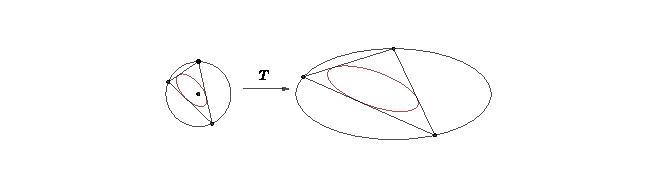
\includegraphics[width=1.0\textwidth]{pics_07_070_Tafim_par_elipses.pdf}
    \caption{Affine image of pair of a Poncelet pair with outer unitary circle having 3-periodics.  }
    \label{fig:07-tafim}
\end{figure}

%\textcolor{red}{ronaldo: organiza, %eu chamaria $p_1$ e $p_2$ talvez %de $X_1$ e de $[e_1,e_2,e_3]$, %mexer no exercicio.}

The above entails yet another alternative proof for the ellipticity of the $X_1$ locus over billiard 3-periodics:

\begin{corollary}
Over billiard 3-periodics, the locus of $X_1$ is given by:
%\[2\,ab{\lambda}^{2}{z}^{2}+2\,\lambda\, \left( {a}^{3}{\lambda}^{2}-{b}
%^{3}{\lambda}^{2}-{a}^{3}-{b}^{3} \right) z+{c}^{2} \left( {c}^{2}{
%\lambda}^{4}-2\,ab{\lambda}^{2}-{c}^{2} \right)=0 \]
 \[   X_1 =z-{\frac { \left( -{a}^{4}+{b}^{4}+{c}^{2}\delta \right) \lambda}{2\,{a
}^{2}{b}^{2}}} -\frac{    ( a^2 + b^2)\delta -a^4 - b^4}{ 2 a^2 b^2 \lambda}=0
\]
%$-\frac{    ( a^2 + b^2)\delta -a^4 - b^4}{ 2 a^2 b^2 \lambda}$
\label{cor:07-X1q2} 
\end{corollary}

\begin{proof}
Let $a$ and $b$ be the semi-axes of the billiard. In the confocal pair 
we have that
\[f={\frac {1}{c}\sqrt { 2\,\delta-{a}^{2}-{b}^{2}}}, \;\; g= -{\frac {1}{c}\sqrt {2\,\delta-{a}^{2}-{b}^{2} }}\]
This is obtained by taking an affine map
$T(z)=(a+b)z/2+(a-b)\bar{z}/2$ sending the pair with an unitary outer circle to the confocal pair, see   \cref{sec:02-caustic}.  

The result follows by factorization of the quartic  polynomial that defines $X_1$ in \cref{prop:07-X1g}.

Using CAS we obtain that $X_1$ is factorizable as $E_1 E_2$, where
{\small  
\begin{align*}
    E_1&=z-{\frac { \left( -{a}^{4}+{b}^{4}+{c}^{2}\delta \right) \lambda}{2\,{a
}^{2}{b}^{2}}} -\frac{    ( a^2 + b^2)\delta -a^4 - b^4}{ 2 a^2 b^2 \lambda}=0
%
\\
    E_2&= -2c^2\lambda\left[-2\,{a}^{2}{b}^{2}\lambda\,{z}^{3}+ \left(  \left( {c}^{2}{\lambda}^{2
}-{a}^{2}-{b}^{2} \right) \delta+{c}^{2} \left( {a}^{2}+{b}^{2}
 \right) {\lambda}^{2}-{a}^{4}+4\,{a}^{2}{b}^{2}-{b}^{4} \right) {z}^{
2}\right.
\\
& \left.   -4\,\lambda\,{c}^{2} \left( {a}^{2}+{b}^{2}+\delta \right) z-4\,{
\lambda}^{2} \left( {a}^{4}+{b}^{4}+{a}^{2}\delta+{b}^{2}\delta
 \right) 
\right]
\end{align*}
}
\end{proof}

\begin{corollary}
The locus $X_1$ is the ellipse with semi-axes given by $a_1=(a^2-\delta)/b$ and $b_1=(\delta-b^2)/a.$

%\[z= {\frac { \left( a-b \right)  \left(\delta -{a}^{2}-ab-{b}^{2}
 %\right) \lambda}{2\,ab}}-{\frac { \left( a+b %\right)  \left(  \delta-{a}^{2}
%+ab-{b}^{2} \right) }{2\,ab\lambda}}\]
 
\end{corollary}

\begin{proof}
Follows directly from  \cref{lem:ell-param} and  \cref{prop:07-X1q2}.
\end{proof}

\begin{remark}
The space of possible choices of two conics which admits a 3-periodic family is five dimensional.
\end{remark}

This stems from the fact that a conic has five degrees of freedom, so two conics have 10; the euclidean transformation group is 4-dimensional, and Cayley deducts one degree of freedom. Therefore: 10-4-1=5.

Note that over said 5d space, the possible confocal configurations are 1-dimensional. Interestingly, experimental evidence suggests that our very first result (elliptic locus of the incenter and excenters) is actually very rare:

\begin{conjecture}
Over Poncelet 3-periodics in a given pair of conics, the locus of the incenter and excenters are ellipses if and only if the pair is confocal.
\label{conj:07-incenter-excenter-loci}
\end{conjecture}

%Evidence also suggests:
%\textcolor{red}{ronaldo is this correct? da uma olhada nos \href{https://bernard-gibert.pagesperso-orange.fr/Tables/table28.html}{strong and weak points do gibert} -- mark sugere investigar se a conjectura certa é nao-racional nos sidelenghts squared}

%\begin{conjecture}
%If a given triangle center $X_k$ has trilinear (or barycentric) coordinates which are irrational on the sidelengths, then the locus of $X_k$ is non-elliptic.
%\end{conjecture}

\input{chap_07/07_060_loci}
\input{chap_07/07_070_circular}
\section{Epilogue: A theory for elliptic loci in the confocal pair}

%The affine transformation  $x\rightarrow{x/a}$, $y\rightarrow{y/b}$ sends the confocal pair to a pair where the outer conic is the unit circle and the caustic $\E_c'$ is a concentric ellipse. The foci $f,g$ of the $\E_c'$ are given by:

%\[ f=(-c',0),\;\;\;g=(c',0) \]

%\noindent where $c'=(1/c)\sqrt{2 \delta -a^2-b^2}$.

\begin{proposition}
If a triangle center $X_k$ is stationary over a Poncelet 3-periodic family, then the locus of any triangle center $\X$ which is a fixed linear combination of $X_2,X_3,X_k$ will be an ellipse. 
\label{prop:07-fixed-lin-comb}
\end{proposition}

\begin{proof}
The triangle center $\X=\alpha X_2+ \beta X_3+ \gamma X_k$ is the linear combination $\X\ab:=\alpha X_2+ \beta X_3$ under a fixed translation by $\gamma X_k$, because both $\gamma X_k$ and $X_k$ are fixed over the family.
\end{proof}

This entails the most compact rendition of the following result (appearing originally in \cite{helman2021-theory}:

\begin{corollary}
Over billiard 3-periodics, the locus of $X_1$ is an ellipse.
\label{cor:07-x1-ellipse}
\end{corollary}

\begin{proof}
For any triangle, $X_1$ can be expressed as the linear combination $X_1=\alpha X_2+\beta X_3+\gamma X_9$ of $X_2$, $X_3$ and $X_9$ with:

\[ \alpha =\frac{6}{\rho+2},\;\;\beta=\frac{2\rho}{\rho+2},\;\;\gamma=\frac{-\rho-4}{\rho+2} \]

\noindent where $\rho=r/R$, is the ratio of inradius to circumradius. Since in the confocal family $X_9$ is stationary and $\rho$ is invariant \cite{reznik2020-intelligencer}, the claim follows.
\end{proof}

Table \cref{tab:07-x1-methods} shows a history of proof techniques of the ellipticity of $X_1$ over billiard 3-periodics:

\begin{table}
\begin{tabular}{|l|c|l|l|}
\hline
Author & Year & Technique  & Reference \\
\hline
D. Reznik        & 2011 & Experimental Video &  \cite{reznik2011-incenter} \\
O. Romaskevich   & 2014 & Complex Analytic  Geometry  &  \cite{olga14}  \\
R. Garcia        & 2016 & Real Analytic   Geometry &  \cite{ garcia2019-incenter}  \\
(in this book)   & 2021 & Specialize $X_1$ locus to confocal pair &  \cref{cor:07-X1q2}  \\
M. Helman et al. & 2021 & 3-Center Linear Combination  &  \cite{helman2021-theory} \\
\hline
\end{tabular}
\caption{Various proof methods for the ellipticity of $X_1$ over billiard 3-periodics.}
\label{tab:07-x1-methods}
\end{table}

We can expand the above result to other triangle centers in the confocal pair, as many of these are fixed linear combinations of $X_2$, $X_3$, and $X_9$. 

\begin{proposition}
In the confocal pair, from $X_1$ to $X_{200}$, the loci of $X_k$ are ellipses, $k=$1,  2,  3,  4,  5,  7,  8,  10,  11,  12,  20,  21,  35,  36,  40,  46,  55,  56,  57,  63,  65,  72,  78,  79,  80,  88$^\dagger$, 84,  90, 100, 104, 119, 140, 142, 144, 145, 149, 153, 162$^\dagger$, 165, 190$^\dagger$, 191, 200.
\end{proposition}

\begin{proof}
As in the previous corollary, one can write $X_1$ as a fixed linear combination of $X_2$, $X_3$, and $X_9$, given that the ratio $\rho=r/R$ is constant in the confocal pair.
In \cite[Table 2
]{helman2021-theory}, a table of fixed coefficients $\alpha,\beta,\gamma$ is provided expressing each of the triangle centers in the claim as fixed linear combinations of $X_1$, $X_2$ and $X_3$. \cref{tab:07-abg} reproduces those results. Therefore all triangle centers in the claim (except for $X_{88}$, $X_{162}$, and $X_{190}$) are fixed linear combinations of $X_1$, $X_2$, and $X_3$, and therefore they are fixed linear combinations of $X_2$, $X_3$, and $X_9$ as well. By \cref{prop:07-fixed-lin-comb}, given that $X_9$ is stationary over the confocal family, this implies the loci of all these triangle centers are ellipses.
\end{proof}

$^\dagger$Note: the loci of $X_{88}$, $X_{162}$, and $X_{190}$ (called ``swans'' before) are also ellipses because by definition they lie on the circumconic centered on $X_9$ \cite[X(9)]{etc}.

\begin{table}
\begin{minipage}{2.0in}
\begin{tabular}{|c|c|c|c|}
\hline
$X_k$ & $\alpha$ & $\beta$ & $\gamma$ \\
\hline$X_1$ &$1$ & $0$ & $0$ \\
$X_2$ & $0$ & $1$ & $0$  \\
$X_3$ & $0$ & $0$ & $1$  \\
$X_4$ & $0$ & $3$ & $-2$ \\
$X_5$ & $0$ & $3$ & $-1$ \\
$X_{7}$ & $\frac{2\rho+4}{\rho+4}$ & $\frac{3\rho}{\rho+4}$ & $\frac{-4\rho}{\rho+4}$  \\
$X_9$ & $\frac{-\rho-2}{\rho+4}$ & $\frac{6}{\rho+4}$ & $\frac{2\rho}{\rho+4}$\\
$X_{10}$ & $1$ & $-3$ & $0$  \\
$X_{11}$ & $\frac{1}{1-2\rho}$ & $\frac{-3\rho}{1-2\rho}$ &  $\frac{\rho}{1-2\rho}$  \\ 
$X_{12}$ & $\frac{1}{1+2\rho}$ & $\frac{3\rho}{1+2\rho}$ &  $\frac{-\rho}{1+2\rho}$  \\ 
$X_{20}$ & $0$ & $3$ & $-4$ \\
$X_{21}$ & $0$ & $\frac{3}{2\rho+3}$ & $\frac{2\rho}{2\rho+3}$  \\
$X_{35}$ & $\frac{1}{2\rho+1}$ &  $0$ & $\frac{2\rho}{2\rho+1}$ \\
$X_{36}$ & $\frac{1}{1-2\rho}$ & $0$ & $\frac{-2\rho}{1-2\rho}$  \\
$X_{40}$ & $1$ & $0$ & $-2$ \\
$X_{46}$ & $\frac{1+\rho}{1-\rho}$ & $0$ & $\frac{-2\rho}{1-\rho}$ \\
$X_{55}$ & $\frac{1}{1+\rho}$ & $0$ & $\frac{\rho}{1+\rho}$  \\
$X_{56}$ & $\frac{1}{1-\rho}$ & $0$ & $\frac{-\rho}{1-\rho}$ \\
$X_{57}$ & $\frac{2+\rho}{2-\rho}$ & $0$ & $\frac{-2\rho}{2-\rho}$  \\
$X_{63}$ & $\frac{-\rho-2}{\rho+1}$ & $\frac{3}{\rho+1}$ &  $\frac{2\rho}{\rho+1}$\\
\hline
\end{tabular}
\end{minipage}
\begin{minipage}{2.0in}
\begin{tabular}{|c|c|c|c|}
\hline
$X_k$ & $\alpha$ & $\beta$ & $\gamma$ \\
\hline
$X_{65}$ & $\rho+1$ & $0$ & $-\rho$ \\ 
$X_{72}$ & $-\rho-2$ & $3$ & $\rho$ \\
$X_{78}$ & $\frac{\rho+2}{\rho-1}$ & $\frac{-3}{\rho-1}$ & $0$ \\ 
$X_{79}$ & 1 & $\frac{6\rho}{2\rho+3}$ & $\frac{-6\rho}{2\rho+3}$ \\ 
$X_{80}$ & $\frac{2\rho+1}{-2\rho+1}$ & $\frac{-6\rho}{-2\rho+1}$ &  $\frac{2\rho}{-2\rho+1}$ \\
$X_{84}$ & $\frac{-\rho-2}{\rho}$ & $\frac{6}{\rho}$ & $\frac{2\rho-4}{\rho}$ \\ 
$X_{90}$ & $\frac{-(\rho+1)^2}{\rho^2+2\rho-1}$ & $\frac{6\rho}{\rho^2+2\rho-1}$ & $\frac{2\rho(\rho-1)}{\rho^2+2\rho-1}$\\ 
$X_{100}$ & $\frac{2}{2\rho-1}$ & $\frac{-3}{2\rho-1}$ & $\frac{2\rho}{2\rho-1}$ \\
$X_{104}$ & $\frac{-2}{2\rho-1}$ & $\frac{3}{2\rho-1}$ & $\frac{2\rho-2}{2\rho-1}$ \\ 
$X_{119}$ & $\frac{1}{2\rho-1}$ & $\frac{3\rho-3}{2\rho-1}$ & $\frac{-\rho+1}{2\rho-1}$ \\
$X_{140}$ & $0$ & $3$ & $1$  \\
$X_{142}$ & $\frac{\rho+2}{2\rho+8}$ & $\frac{3\rho+6}{2\rho+8}$ & $\frac{-2\rho}{2\rho+8}$ \\
$X_{144}$ & $\frac{4\rho+8}{-\rho-4}$ & $\frac{3\rho-12}{-\rho-4}$ & $\frac{-8\rho}{-\rho-4}$\\
$X_{145}$ & $4$ & $3$ & $0$ \\
$X_{149}$ & $\frac{-4}{6\rho-3}$ &  $\frac{9-6\rho}{6\rho-3}$ &  $\frac{12\rho-8}{6\rho-3}$ \\
$X_{153}$ & $\frac{4}{6\rho-3}$ & $\frac{-6\rho-3}{6\rho-3}$ & $\frac{12\rho-4}{6\rho-3}$ \\
$X_{165}$ & $1$ & $0$ & $-4$ \\
$X_{191}$ & $-1$ & $\frac{6}{2\rho+3}$ & $\frac{4\rho}{2\rho+3}$ \\
$X_{200}$ & $\frac{\rho+4}{\rho-2}$ & $\frac{-6}{\rho-2}$ & $0$ \\
\hline
\end{tabular}
\end{minipage}
\caption{Coefficients $\alpha,\beta,\gamma$ used to express $X_k$ as the linear combinations $\alpha X_1+\beta X_2+\gamma X_3$. Note: $\rho=r/R$. Note also that although though the loci of $X_{88}$, $X_{162}$, and $X_{190}$ are ellipses (they sweep the elliptic billiard), they are cannot be expressed fixed linear combinations of $X_1,X_2,X_3$. Notice $\alpha$,$\beta$,$\gamma$ are the same up to sign of $\rho$ for harmonic conjugate pairs ($X_{11}$,$X_{12}$), ($X_{35}$,$X_{36}$), ($X_{55}$,$X_{56}$).}
\label{tab:07-abg}
\end{table}

Referring to \cref{fig:07-confocal-degenerate}:

\begin{proposition}
In the confocal pair, the locus of $\X=\alpha X_2+\beta X_3$ for $\alpha,\beta\in\R$ is a circle when:

\[\left(\frac{\alpha}{\beta}\right)_{\pm}=\frac{\delta-3 a b\pm 2\left(a^2+b^2\right)}{2 a b} \]
\end{proposition}

\begin{proof}
By \cref{lem:ell-param}, this will happen when $|u|+|v|=\big||u|-|v|\big|$ with $u,v$ from \cref{thm:07-ellipse-locus}. In the confocal pair, when $\alpha,\beta\in\R$, both $u$ and $v$ are real numbers as well. Thus, this condition holds if and only if either $u=0$ or $v=0$. The ratios $\alpha/\beta$ that yield circular loci can then be computed directly.
\end{proof}

\begin{observation}
It follows that $\left({\alpha}/{\beta}\right)_+ +\left({\alpha}/{\beta}\right)_-=-3$.
\end{observation}

\begin{definition}[Degenerate Locus] When the elliptic locus of a triangle center is a segment, i.e., one of its axes has shrunk to zero, we will call it ``degenerate''.
\end{definition}

\begin{proposition}
Let $\X$ be a fixed linear combination of $X_2$, $X_3$, and $X_k$, where $X_k$ is some stationary center over the family of 3-periodics. As the vertices of the 3-periodics sweep the outer ellipse monotonically, the path of $\X$ in its elliptical locus is monotonic as well, except for when this locus is degenerate.
\end{proposition}

\begin{proof}
By \cref{thm:07-ellipse-locus}, the locus of $\X$ can be parametrized by $u \l+v\frac{1}{\l}+w$ for some $u,v,w\in\mathbb{C}$, where $\l$ sweeps the unit circle in $\mathbb{C}$ in the same direction as the 3-periodic vertices sweep the outer ellipse of the Poncelet pair. We can thus parametrize $\X$ as $\X(t)=u e^{i t}+v e^{-i t}+w$. If either $u=0$ or $v=0$, it is clear from this parametrization that $\X$ sweeps its locus monotonically. Thus, we can now assume that $u\neq0$ and $v\neq0$.

Denoting $u=u_0+i u_1$ and $v=v_0+i v_1$ with $u_0,u_1,v_0,v_1\in\R$, we can directly compute
\[
    \left|\frac{d}{d t}\X(t)\right|^2= |u|^2+|v|^2 + 2 \sin (2 t) (u_2 v_1-u_1 v_2)-2 \cos (2 t) (u_1 v_1+u_2 v_2)
\]

Since $(u_2 v_1-u_1 v_2)^2+(u_1 v_1+u_2 v_2)^2=(u_1^2+u_2^2)(v_1^2+v_2^2)=|u|^2|v|^2$, there is some angle $\phi\in[0,2\pi)$ (the angle between the vectors $(u_1,u_2)$ and $(v_1,v_2)$) such that $u_1 v_1+u_2 v_2=|u| |v|\cos\phi$ and $u_2 v_1-u_1 v_2=|u| |v|\sin\phi$. Substituting this back in the previous equation, we derive
\begin{gather*}
     \left|\frac{d}{d t}\X(t)\right|^2=|u| |v|\left(\frac{|u|}{|v|}+\frac{|v|}{|u|}+2\sin(2t)\sin(\phi)-2\cos(2t)\cos(\phi)\right)=\\
     =|u| |v|\left(\frac{|u|}{|v|}+\frac{|v|}{|u|}-2\cos(2t+\phi)\right)\geq |u| |v|\left(\frac{|u|}{|v|}+\frac{|v|}{|u|}-2\right)
\end{gather*}

By AM-GM inequality, this last quantity is always strictly greater than 0 unless $|u|=|v|$. If $|u|\neq|v|$, we will have $\left|\frac{d}{d t}\X(t)\right|^2>0$, and hence the velocity vector never vanishes, meaning that the $\X$ sweeps its smooth locus monotonically. By \cref{lem:ell-param}, this means that $\X$ sweeps its locus monotonically except when this locus is degenerate.

\end{proof}

\begin{figure}
    \centering
    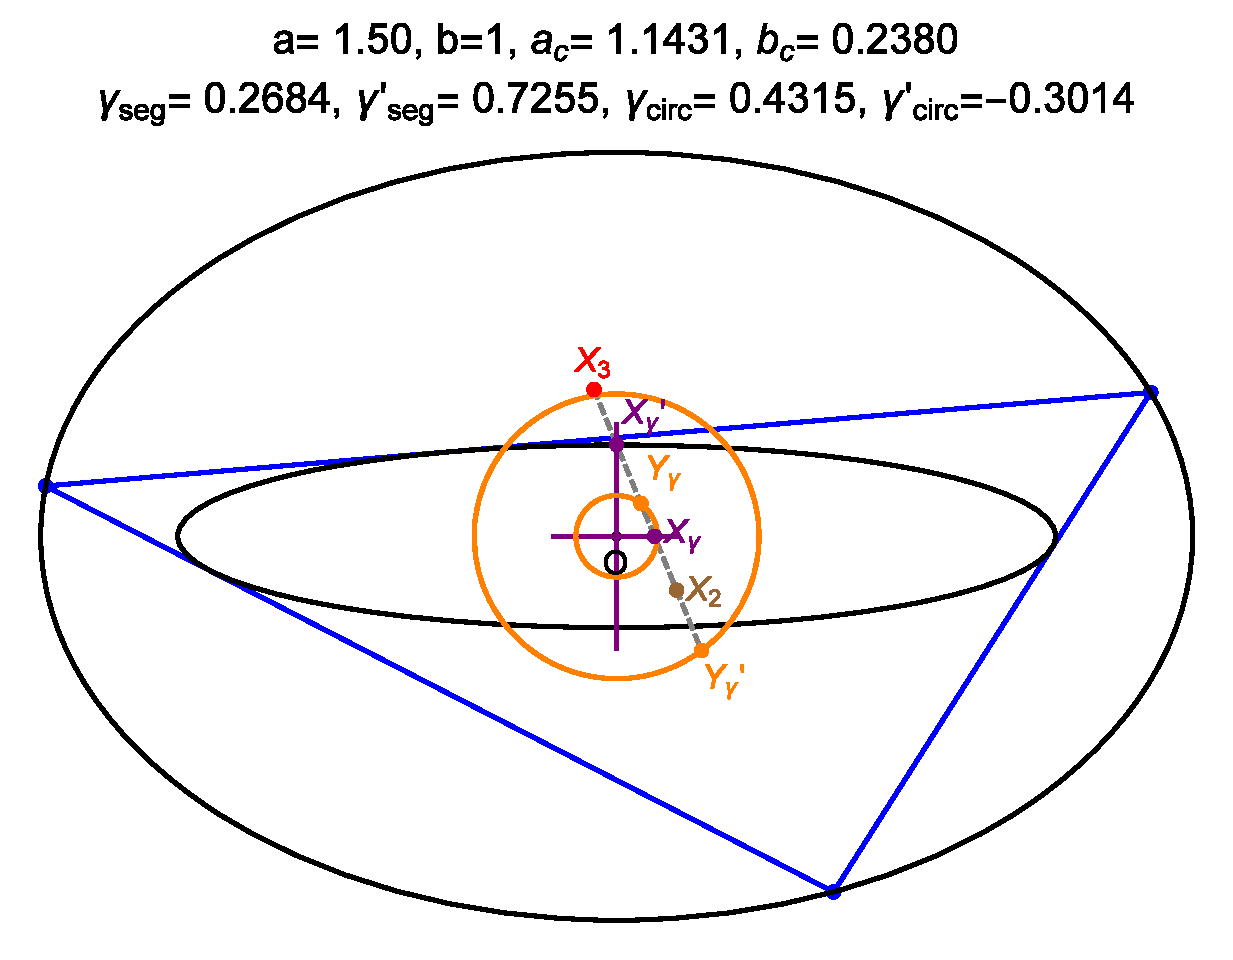
\includegraphics[width=.7\textwidth]{pics_07_060_confocal_degenerate_circle_gammas}
    \caption{A 3-periodic (blue) in a pair of confocal ellipses (black) with $a/b=1.5$. Also shown are two degenerate (segment-like) loci (purple) obtained with $\gamma{\simeq}\{.27,.73\}$ and two circular loci (orange), obtained with $\gamma{\simeq}\{.43,-.3\}$. \href{https://youtu.be/haFTsq5UyK4}{Video}}
    \label{fig:07-confocal-degenerate}
\end{figure}

In \cref{sec:05-triple-winding} we provided a continuity argument for the three turns executed by a triangle center over a traversal of the billiard 3-periodic family.

\begin{remark}
In \cite[Lemma 3.4, p. 28]{daepp-2019} it is shown that (i) the complex argument of the Blaschke product is monotonic on the unit circle, and that (ii) for each $\lambda$ there are 3 solutions for the equation $B(z)=\lambda$. This means that as $\lambda$ sweeps the unit circle monotonically, the 3-periodics sweep the outer Poncelet ellipse monotonically and in the same direction as $\lambda$. Moreover for every 3 full cycles of $\lambda$ over the complex the unit circle, each vertex of the 3-periodics sweep the outer ellipse exactly once.
\label{rem:monotone-Blaschke}
\end{remark}

\begin{proposition}
Let $\X$ be a fixed linear combination of $X_2$, $X_3$, and $X_k$, where $X_k$ is some stationary center over the family of 3-periodics. Over a full cycle of 3-periodics, the winding number of $\X$ over its elliptical locus is $\pm 3$, except for when this locus is degenerate.
\end{proposition}



\begin{proof}
By \cref{thm:07-ellipse-locus}, the locus of $\X$ can be parametrized by $u \l+v\frac{1}{\l}+w$ for some $u,v,w\in\mathbb{C}$. From \cref{rem:monotone-Blaschke}, one can see that the winding number of $\lambda$ associated to 3-periodics is $+3$ for each full cycle of 3-periodics over the outer Poncelet ellipse. Thus, it is sufficient to prove that the winding number of $\X$ over its elliptical locus is $\pm 1$ as $\lambda$ goes around the complex unit circle just once.

Since $w$ is the center of the elliptic locus of $\X$ (see \cref{lem:ell-param}), we compute the winding number of $\X$ around $w$. Parametrizing $\X$ as $\X(t)=u e^{i t}+v e^{-i t}+w$ where $\lambda=e^{i t}$, one can directly compute the winding number as \cite[Lemma 1, p. 114]{ahlfors1979-complex}:

\[
    \frac{1}{2\pi i}\oint_{\X}\frac{d\zeta}{\zeta-w}=\frac{1}{2\pi i}\int_0^{2\pi} \frac{\X'(t)}{\X(t)-w}d t={\mathop{\mathrm{sign}}}(|u|^2-|v|^2)
\]

By \cref{lem:ell-param}, the only way we can have $|u|=|v|$ is if the locus of $\X$ is degenerate. Thus, whenever this locus is not degenerate, the winding number of $\X$ around its locus as $\lambda$ sweeps the unit circle once is equal to $1$ if $|u|>|v|$ and $-1$ when $|u|<|v|$, as desired.
\end{proof}
\section{Exercises}
\label{sec:07-exercises}

\begin{exercise}
Consider a cubic polynomial $p(z)=(z-\alpha_1)(z-\alpha_2)(z-\alpha_3)$ with simple roots $\alpha_i$ (i=1,2,3).
Let $\beta_1$ and $\beta_2$ the roots of $p'(z)$.
Consider the family of confocal ellipses having foci $\beta_1$ and $\beta_2$.

Show that there exists a unique ellipse $\mathcal E$ in this family passing through the midpoints $(\alpha_i+\alpha_j)/2$, and that it is tangent to the sides of the triangle $T=\{\alpha_1,\alpha_2,\alpha_3\}$. This ellipse is known as Steiner innelipse of $T$.

Conclude that the center of $\E$ is the triangular center  $X_2$ of $T$ and that $T$ is a 3-periodic orbit of a homothetic Poncelet pair.
\end{exercise}

\begin{exercise} Consider an ellipse $\E$ and the set of tangent lines. Show that the set of points of intersection between any two perpendicular
tangents to $\E$  lie on a circle. Find the radius and the center of this circle.
\end{exercise}

\begin{exercise}
Consider a circle $\mathcal{C}$ and a point $P_0$.   Consider the family of circles passing through $P_0$ and internally tangent to $\mathcal{C}$. Show that the set of centers of this family of circles is an ellipse.
Find the semi-axes and the foci of the ellipse.
\end{exercise}

\begin{exercise}
In the proof of \cref{prop:07-X1q2}, let $z_1(\lambda)$, $ z_2(\lambda) $ and $z_3(\lambda)$ the roots of   $E_2(z,\lambda)=0$, $\lambda \in \mathbb{T}$. Show that  the trace of these three curves is an ellipse, i.e., they parametrize the excentral locus.   
\end{exercise}

\begin{exercise}
Consider a triangle inscribed in $\T^1$ with vertices $w_1^2$, $w_2^2$ and $w_3^2$. Show that:
\begin{itemize}
\item The incenter $X_1$ is $-w_1w_2-w_1w_3-w_2w_3$.
\item  The excenters are 
$w_1w_2-w_1w_3-w_2w_3$,\, $-w_1w_2+w_1w_3-w_2w_3$ and $-w_1w_2-w_1w_3+w_2w_3$.
\item The barycenter  $X_2$ is
$(w_1^2+w_2^2+w_3^2)/3$.
\item The orthocenter $X_4$ is
$w_1^2+w_2^2+w_3^2$.
\item The nine-point center $X_5$   is $(w_1^2+w_2^2+w_3^2)/2$.
\end{itemize}
\label{exe:05-X1}
\end{exercise}

\begin{exercise}
Derive the conditions under which a locus of a triangle center becomes degenerate (segment-like) over billiard 3-periodics.
\end{exercise}
\section{Research Questions}
\label{sec:07-research}

\begin{question}
In \cref{que:02-extouch} one is asked to prove that the family of billiard 3-periodic extouch triangles is Ponceletian. Prove that over this family the loci of $X_k$, $k=2,3,4,5,20$ are ellipses, derive their semi-axes. See it \href{https://bit.ly/2RdtlvH}{Live}.
\end{question}

\begin{question}
Prove \cref{conj:07-incenter-excenter-loci}.
\end{question}

\begin{question}
Prove (or disprove) \cref{conj:07-locus}.
\end{question}

\begin{question}
Recall 3-periodics in the Brocard porism, \cref{sec:04-broc-porism}. The Brianchon point of the Brocard inellipse is (stationary) $X_6$, i.e., family sidelines touch the inellipse at the vertices of the $X_6$-cevian, in \cite{mw} called the {\em symmedial} triangle \cite{mw}. Show  that over Brocard porism 3-periodics, (i) the symmedial triangles are Ponceletian, (ii) compute the center and semi-axes of its inellipse, (iii) show that the locus of $X_k$, $k=13,14,15,16$ are circles. See it \href{https://bit.ly/3hXos4E}{Live}.
\end{question}

\chapter{Experimental Techniques}
\label{chap:08-experimental}
%We call {\em focus-inversive} (or simply {\em inversive}) the family of triangles which are the inversive image of billiard N-periodics with respect to a circle centered on a focus. The $N=3$ case is shown in \cref{fig:08-n3-finv}.

Note that since the inversive image of an ellipse with respect to a focus is a loopless Pascal's Limaçon, see \cite{mw}, the focus-inversive is inscribed in such a curve ans is therefore not Ponceletian. Indeed, the caustic is also non-elliptic. As shown in \cref{fig:08-n3-caustics}, a continuously increasing billiard aspect ratio will transition the caustic from (i) a regular curve, to (ii) one with a self-intersection and two cusps, to (iii) a non-compact curve with two infinite branches.

\begin{figure}
    \centering
    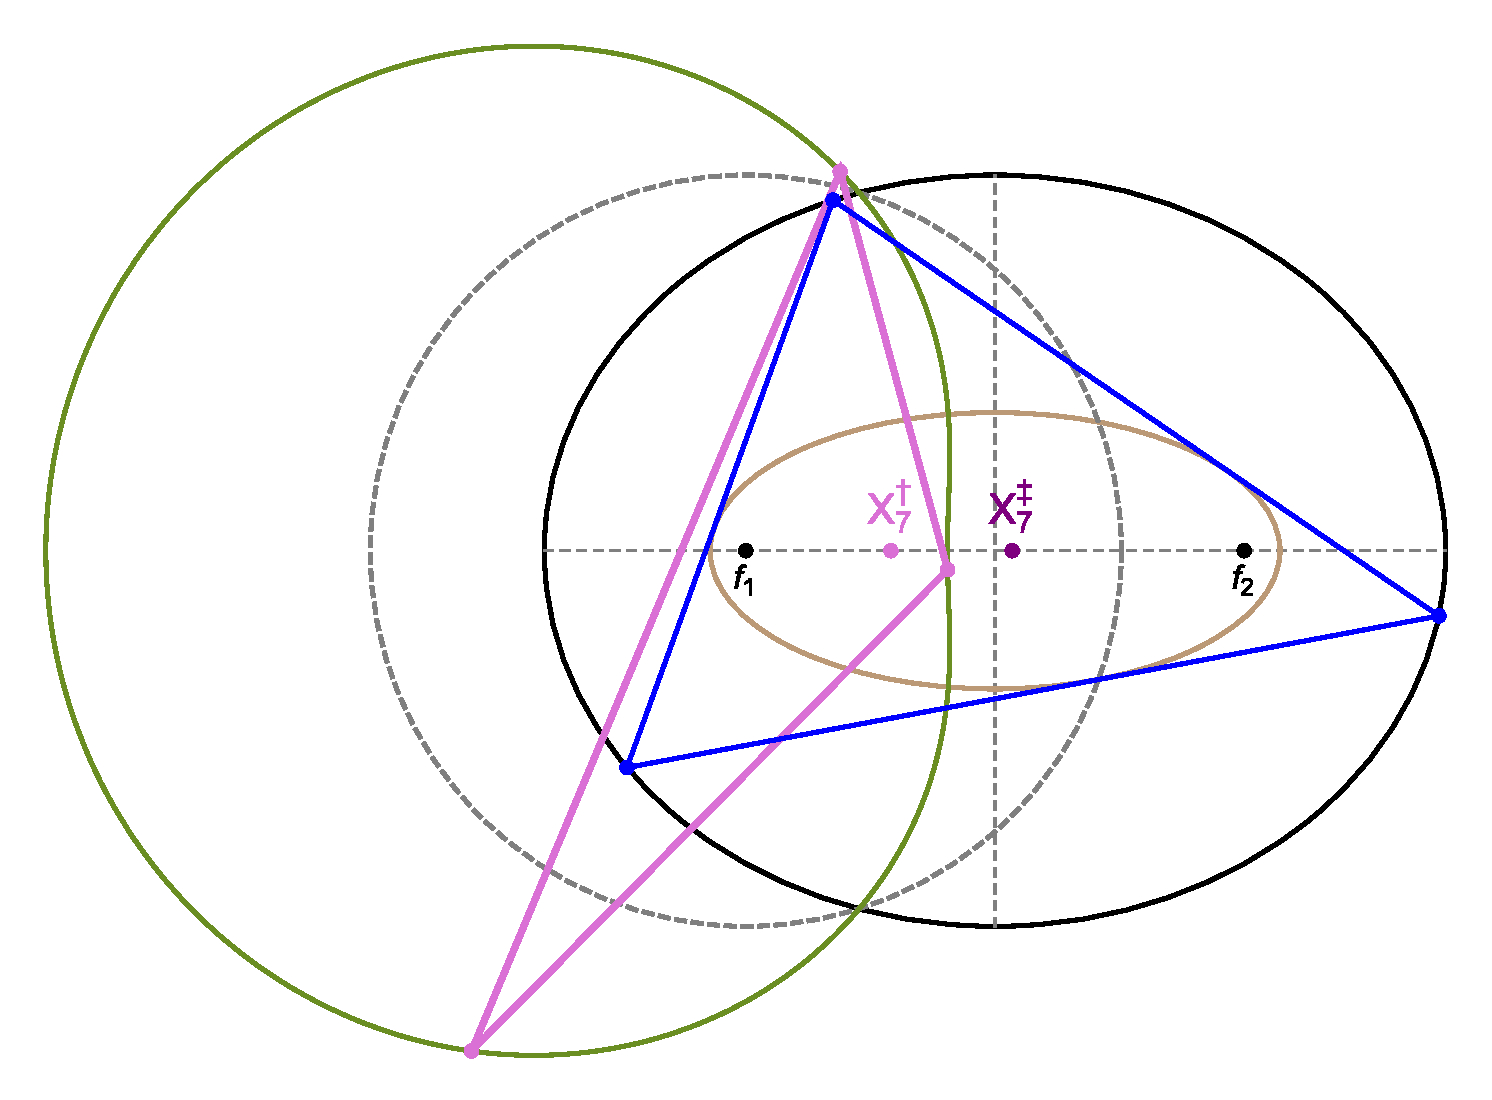
\includegraphics[width=.8\textwidth]{pics_08_010_n3_finv.eps}
    \caption{The $N=3$ focus-inversive family (pink), i.e., the inversive image of billiard 3-periodics (blue) with respect to a focused-centered circle $\Cm$ (dashed gray). Focus-inversives are inscribed in a loopless Pascal's Limaçon (olive green). Both perimeter and sum of cosines are invariant. The Gergonne point $X_7^\dagger$ is stationary. Also shown is $X_7^\ddagger$, the inversive image of $X_7^\dagger$ with respect to $\Cm$, inquired about in \cref{exe:08-x7-ddagger}. \href{https://bit.ly/3i19g6Q}{Live}}
    \label{fig:08-n3-finv}
\end{figure}

\begin{figure}
    \centering
    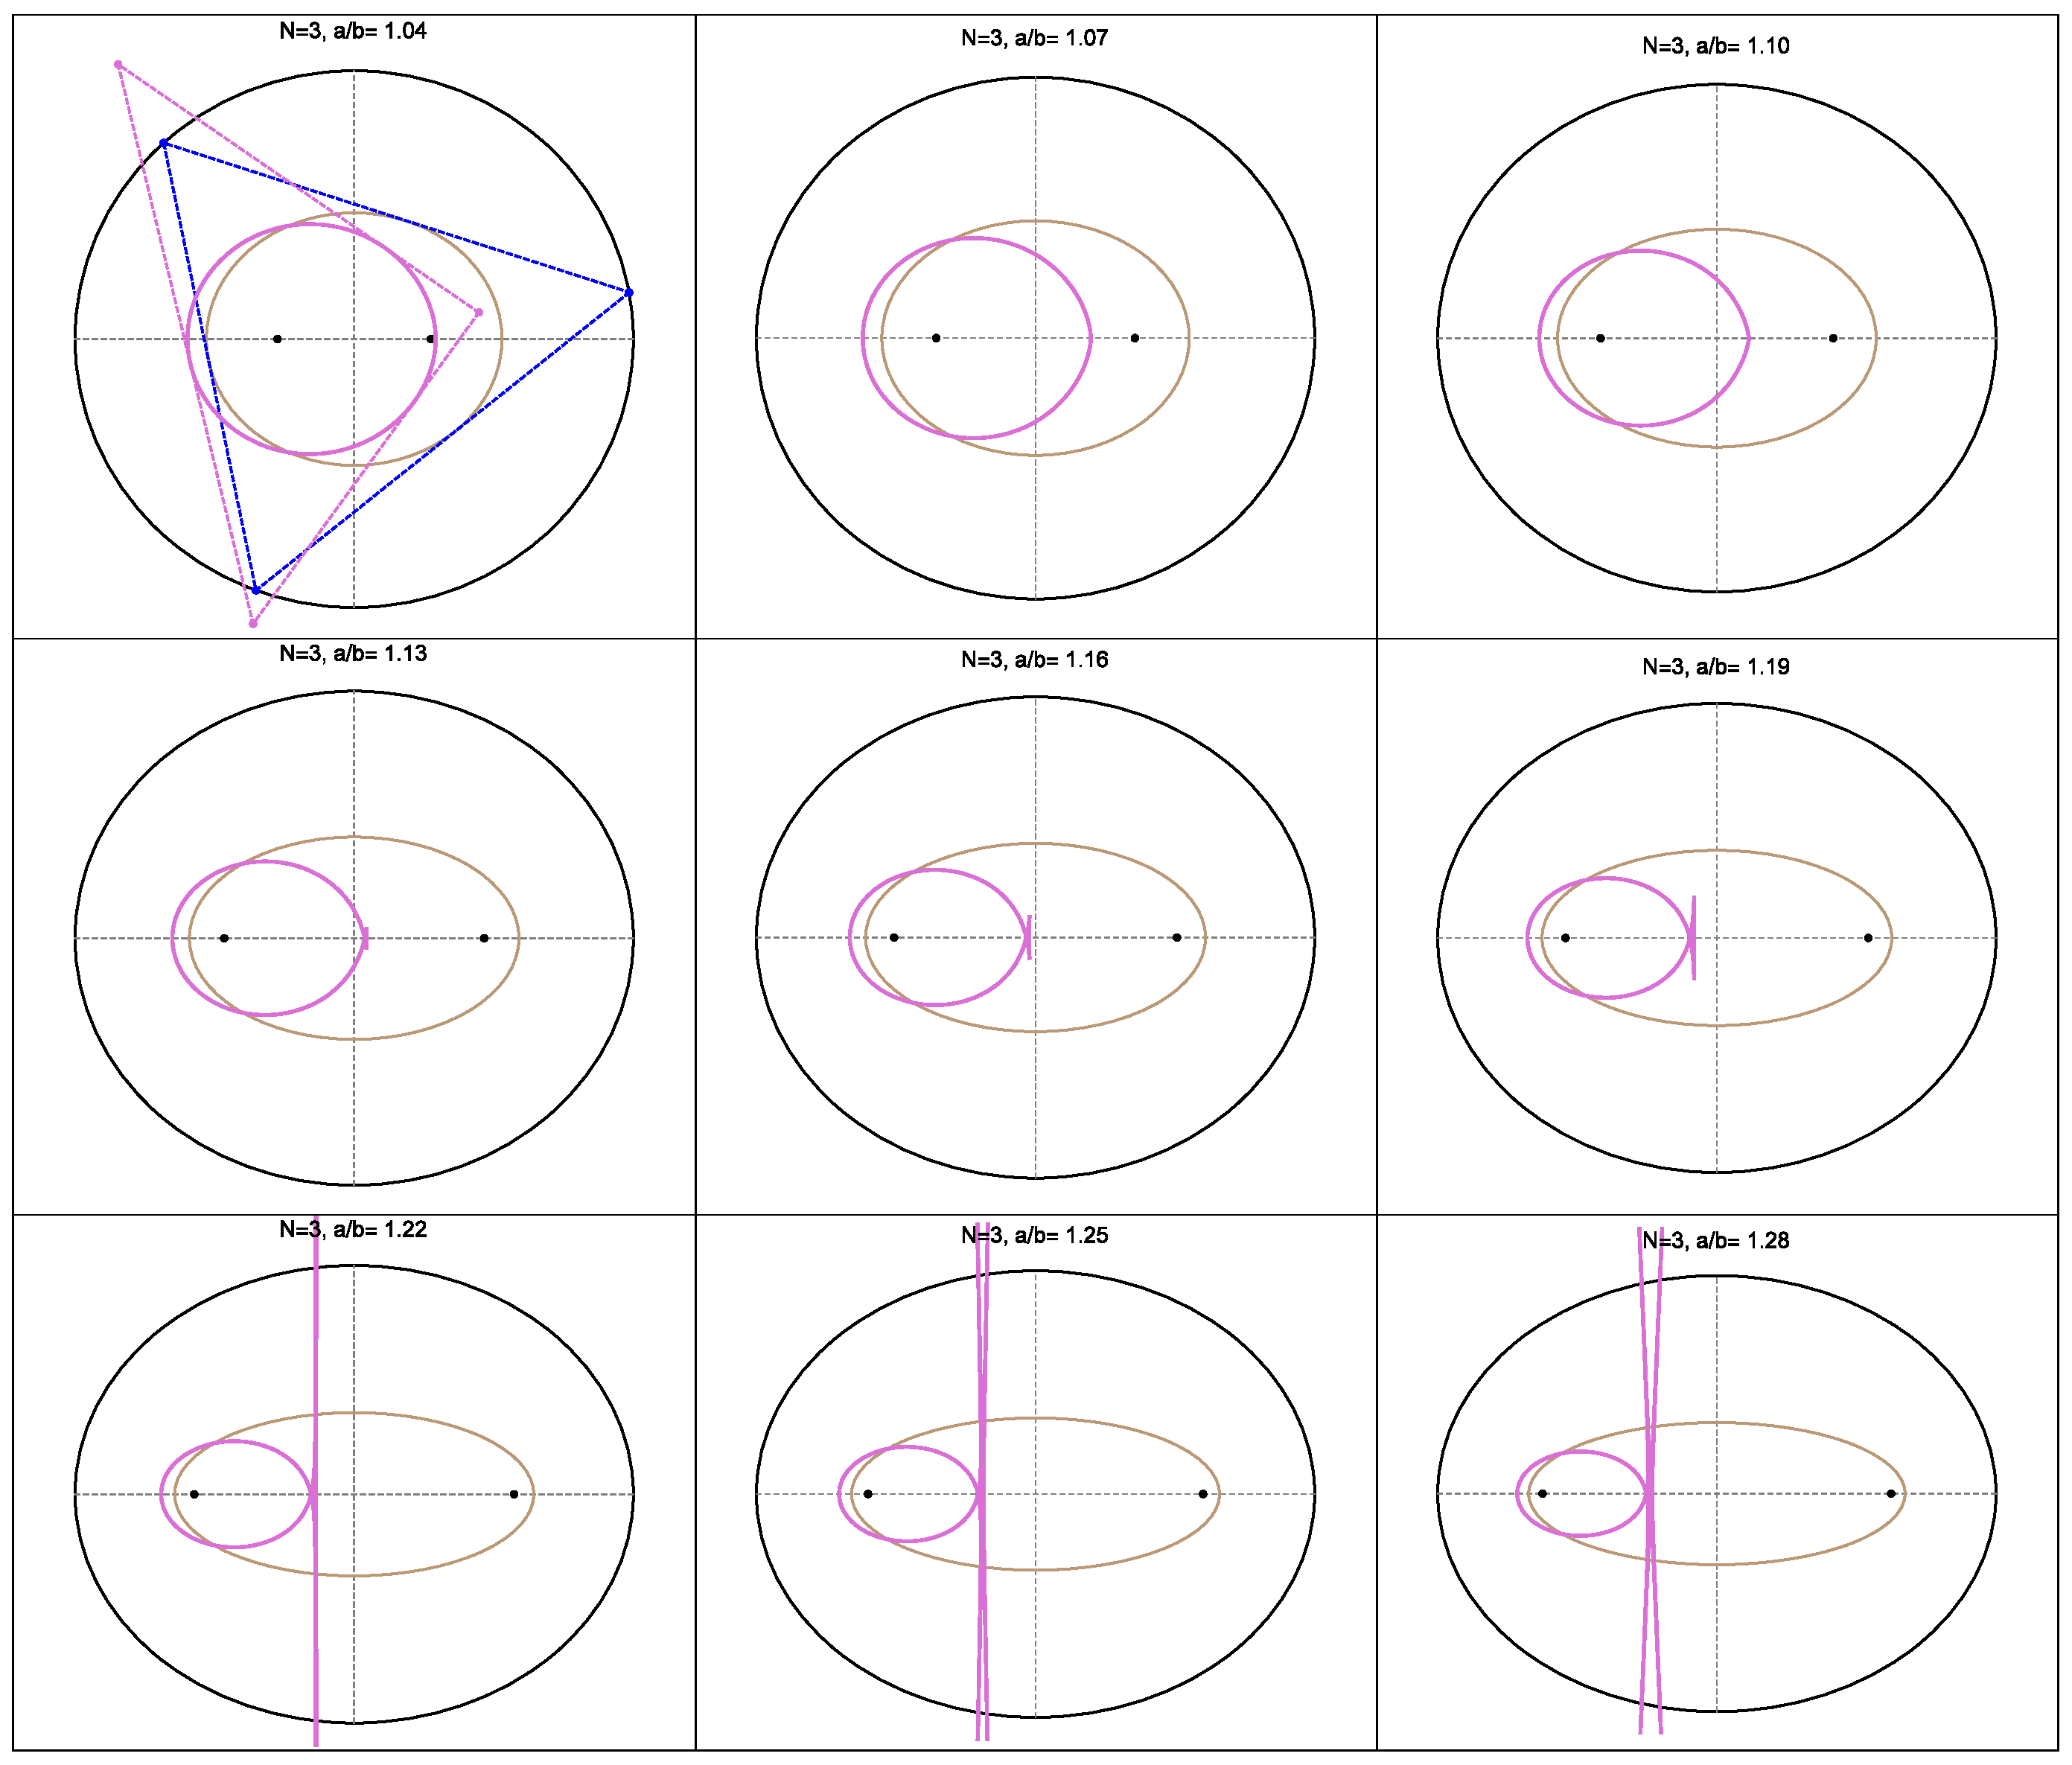
\includegraphics[width=\textwidth]{pics_08_020_n3_caustic.eps}
    \caption{Non-conic caustic (pink) to the focus-inversive family (pink). A billiard 3-periodic (dashed blue) and the corresponding focus-inversive triangle are shown at the top-left picture only. The billiard caustic is shown on every frame (brown). From left-to-right, top-to-bottom, $a/b$ is increased in small steps. Over this range, the caustic transitions from (i) a regular curve, to (ii) a curve with one self-intersection and two cusps, to (iii) a non-compact curve.  \href{https://bit.ly/374jbBl}{Live}}
    \label{fig:08-n3-caustics}
\end{figure}

\section{A stationary point}

Recall in the confocal family the Mittenpunkt $X_9$ is stationary. Henceforth we shall append a $\dagger$ to all quantities referring to the focus-inversive family. Let $a,b$ denote the semi-axes of the pre-inversion billiard which we assume to be centered on $[0,0]$ and be axis-parallel to $x$, and $y$ respectively. Let $\rho$ denote the radius of $f_1=[-c,0]$, the (left) focus-centered inversion circle, $c^2=a^2-b^2$. Interestingly:

\begin{proposition}
The Gergonne point $X_7^\dagger$ of focus-inversives is stationary on the major axis of the pre-image confocal pair. Its coordinates are given by:
\[ X_7^\dagger=\left[c\left(1-\frac{\rho^2}{\delta+c^2}\right),0\right]\]
where as before: $\delta^2=a^4-(a b)^2+b^4$.
\label{prop:08-gergonne}
\end{proposition} 

\section{Billiard-like invariants}

The following two surprising invariants -- constant perimeter and sum of cosines -- are analogues to those displayed by billiard 3-periodics. Interestingly they are not consequences of elementary principles or transformations. 

\begin{proposition}
The perimeter $L^\dagger$ of focus-inversives is invariant and given by: 
\[L^\dagger=\rho^2 \frac {\sqrt { \left( 8\,{a}^{4}+4\,{a}^{2}{b}^{2}+2\,{b}^{4}
 \right) \delta+8\,{a}^{6}+3\,{a}^{2}{b}^{4}+2\,{b}^{6}}}{{a}^{2}{b}^{
2}}\]
\label{prop:08-inv-perimeter}
\end{proposition}

Let $\theta_i^\dagger$ denote angles internal to focus-inversives. 

\begin{proposition}
The sum of internal angle cosines of focus-inversives is invariant and given by: 
\[
\sum\cos{\theta_{1,i}^\dagger}=\frac{\delta (a^2+c^2-\delta)}{a^2c^2} \]
\label{prop:08-inv-cos-sum}
\end{proposition}

\section{The rotating billiard table}

Recall that in \cref{fig:02-circumbilliard} we introduced the concept of the {\em circumbilliard}: given a triangle $T$, this is the $X_9$-centered circumellipse of which $T$ is a billiard 3-periodic (circumellipse normals are angular bisectors). Let  $\mathcal{C}^\dagger$ denote the (moving) circumbilliard ($X_9^\dagger$-centered circumellipse) of focus-inversives. Indeed, and referring to \cref{fig:08-moving-billiard-table}, focus-inversives are billiard 3-periodics of a rigidly-moving virtual elliptic billiard (see \cref{exe:08-moving-billiard-table}):

\begin{proposition}
Over focus-inversives, the semi-axes $a^\dagger,b^\dagger$ of $\mathcal{C}^\dagger$ are invariant and given by:

\begin{align*}
    a^\dagger&= \rho\,k_1
\sqrt {k_2\left(\delta+a\,c\right)}\\
    b^\dagger&= \rho\,k_1
\sqrt {k_2\left(\delta-a\,c\right) }\\
 \mbox{where:}&\\
k_1&=\frac{c \sqrt{2}}{k_3}\sqrt { \left( 8\,{a}^{4}+4\,{a}^{2}{b}^{2}+2\,{b}^{4}
 \right) \delta+8\,{a}^{6}+3\,{a}^{2}{b}^{4}+2\,{b}^{6}}\\
 k_2&=2 a^2-b^2-\delta\\
 %\sqrt{ \left( -4\,{a}^{2}+2\,{b}^{2} \right) \delta+5\,{a}^{4}-5\,{a}^{2}{b}^{2}+2\,{b}^{4}}\\
k_3&=2a  {b}^{2} \left(  \left( 2\,{a}^{2}-{b}^{2} \right) \delta+2
\,{a}^{4}-2\,{a}^{2}{b}^{2}-{b}^{4}\right)
\end{align*}
\end{proposition}

\begin{figure}
    \centering
    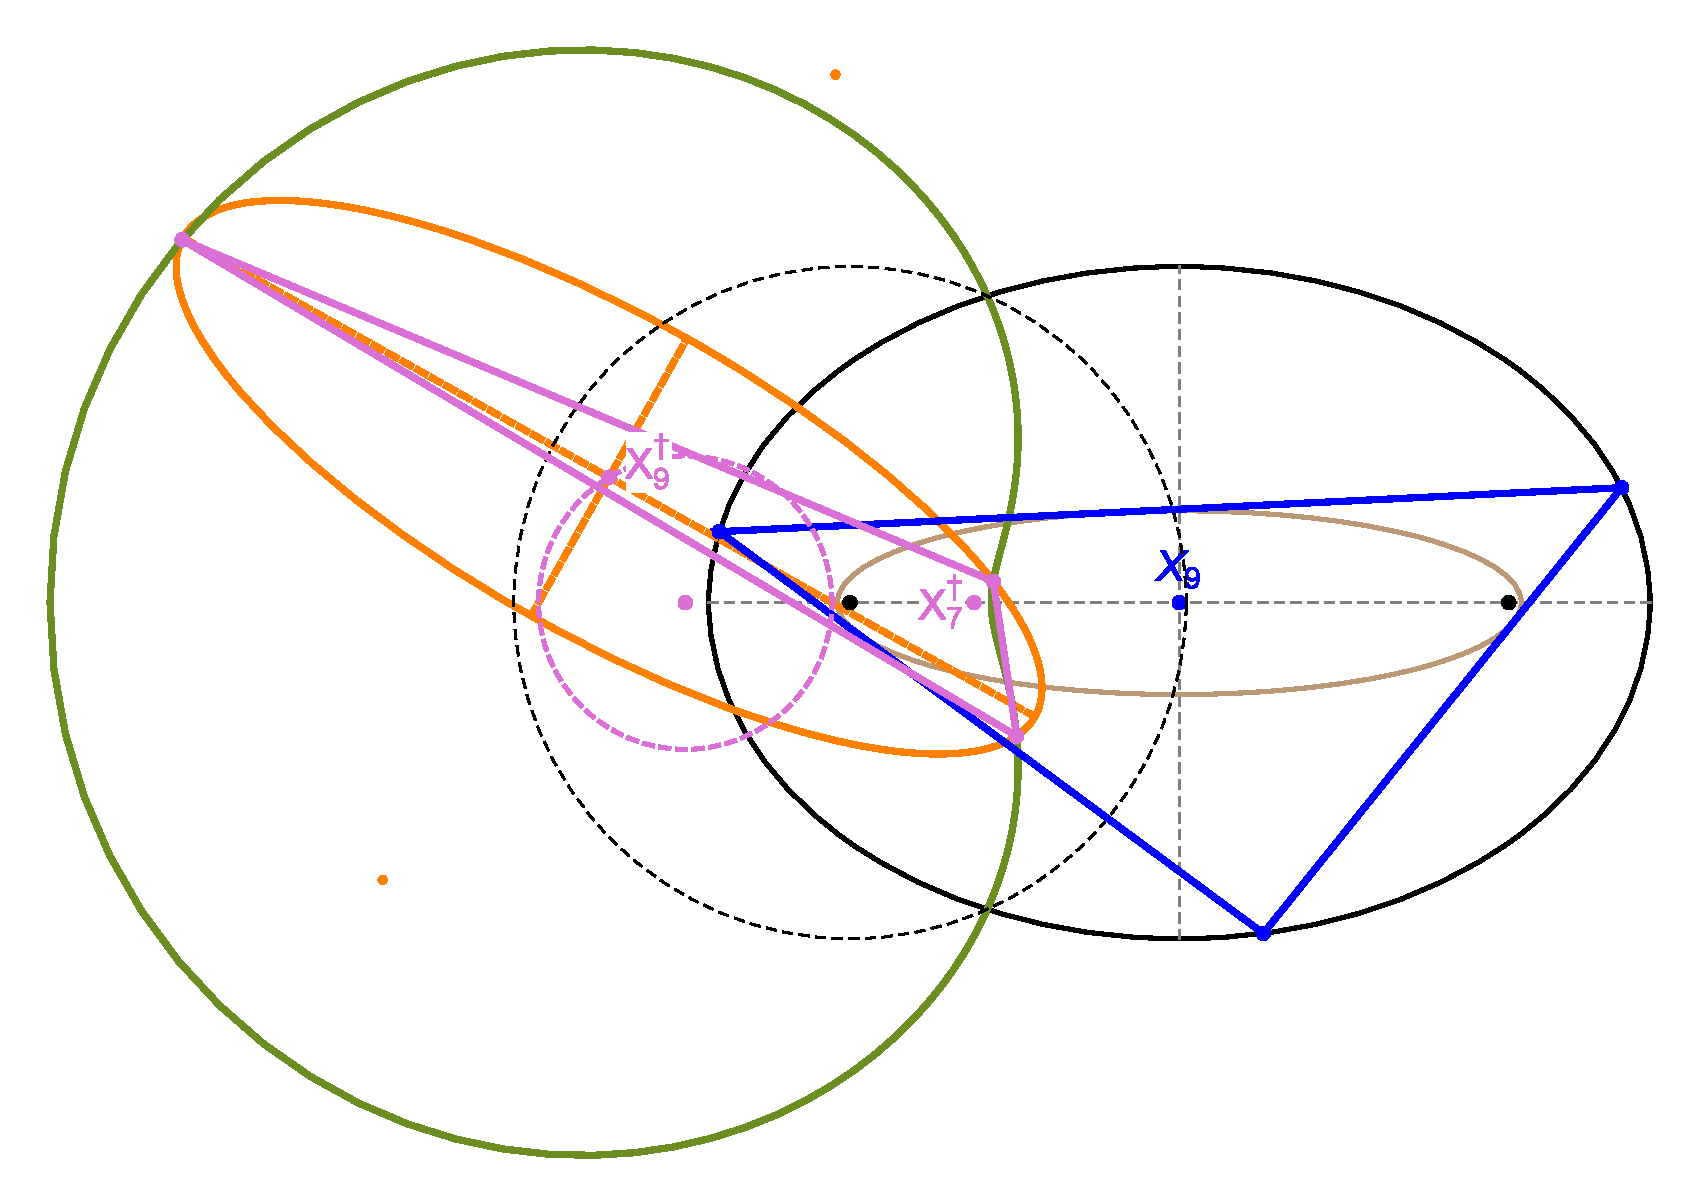
\includegraphics[width=\textwidth]{pics_08_030_n3_rotating_billiard.eps}
    \caption{The moving circumbilliard (orange) to focus-inversives (pink) rigidly translate and rotate (invariant semi-axes). Their center $X_9^\dagger$ sweeps a circle. The location of the stationary Gergonne point $X_7^\dagger$ is also shown. \href{https://youtu.be/LOJK5izTctI}{Video 1}, \href{https://youtu.be/Y-j5eXqKGQE}{Video 2}}
    \label{fig:08-n3-moving-billiard-table}
\end{figure}

\section{Invariant area product}

Let $A_1^\dagger$ (resp. $A_2^\dagger$) denote the area of the $f_1$- (resp. $f_2$) inversive triangle family. Referring to Figure~\ref{fig:08-inv-pedals}:

\begin{proposition}
For $N=3$, the area product $A_1^\dagger A_2^\dagger$ of the two focus-inversive triangles is given by:

\[ A_1^\dagger A_2^\dagger= \frac{\rho^8}{8 a^8 b^2}  \left[\left( {a}^{4}+2\,{a}^{2}{b}^{2}+4\,{b}^{4} \right)\delta +  \frac{3 a^{4} b^{2}}{2}+a^6+4\,{b}^{6} \right]
\]
\end{proposition}

\begin{figure}
    \centering
    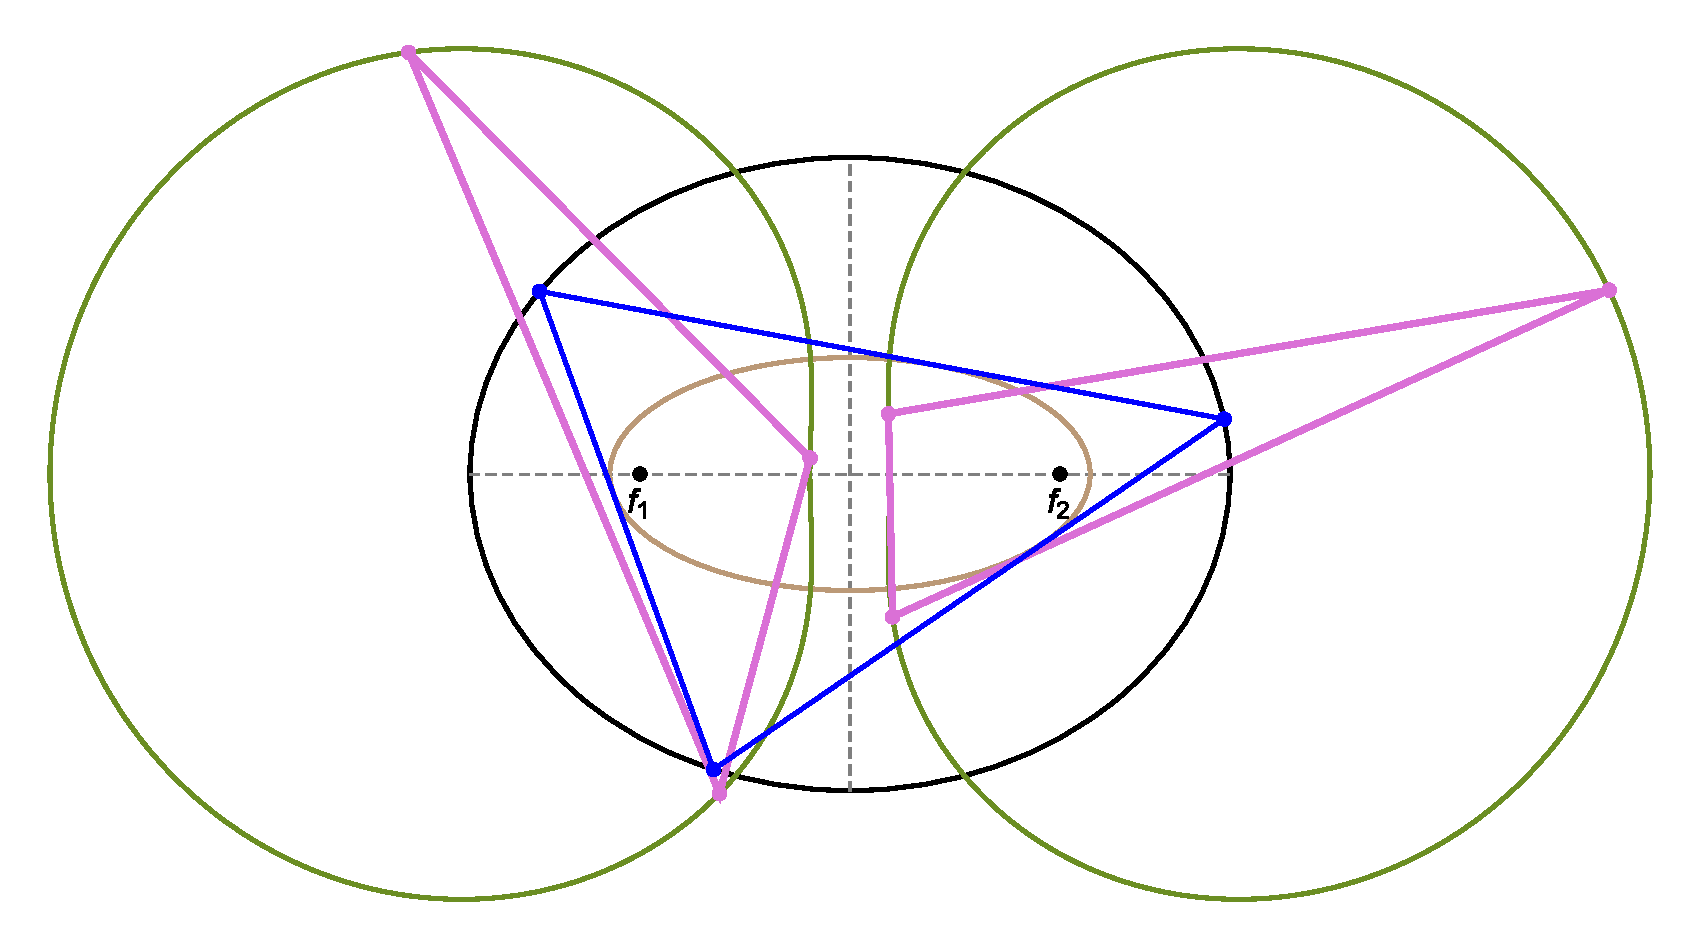
\includegraphics[width=\textwidth]{pics_08_040_n3_f1f2.eps}
    \caption{The area product of $f_1$- and $f_2$-inversive triangles (pink) is invariant. \href{https://youtu.be/0L2uMk2xyKk}{Video}, \href{https://bit.ly/3i1iPCM}{Live}}
    \label{fig:08-inv-pedals}
\end{figure}

\section{Circular loci galore!}

\begin{figure}
    \centering
    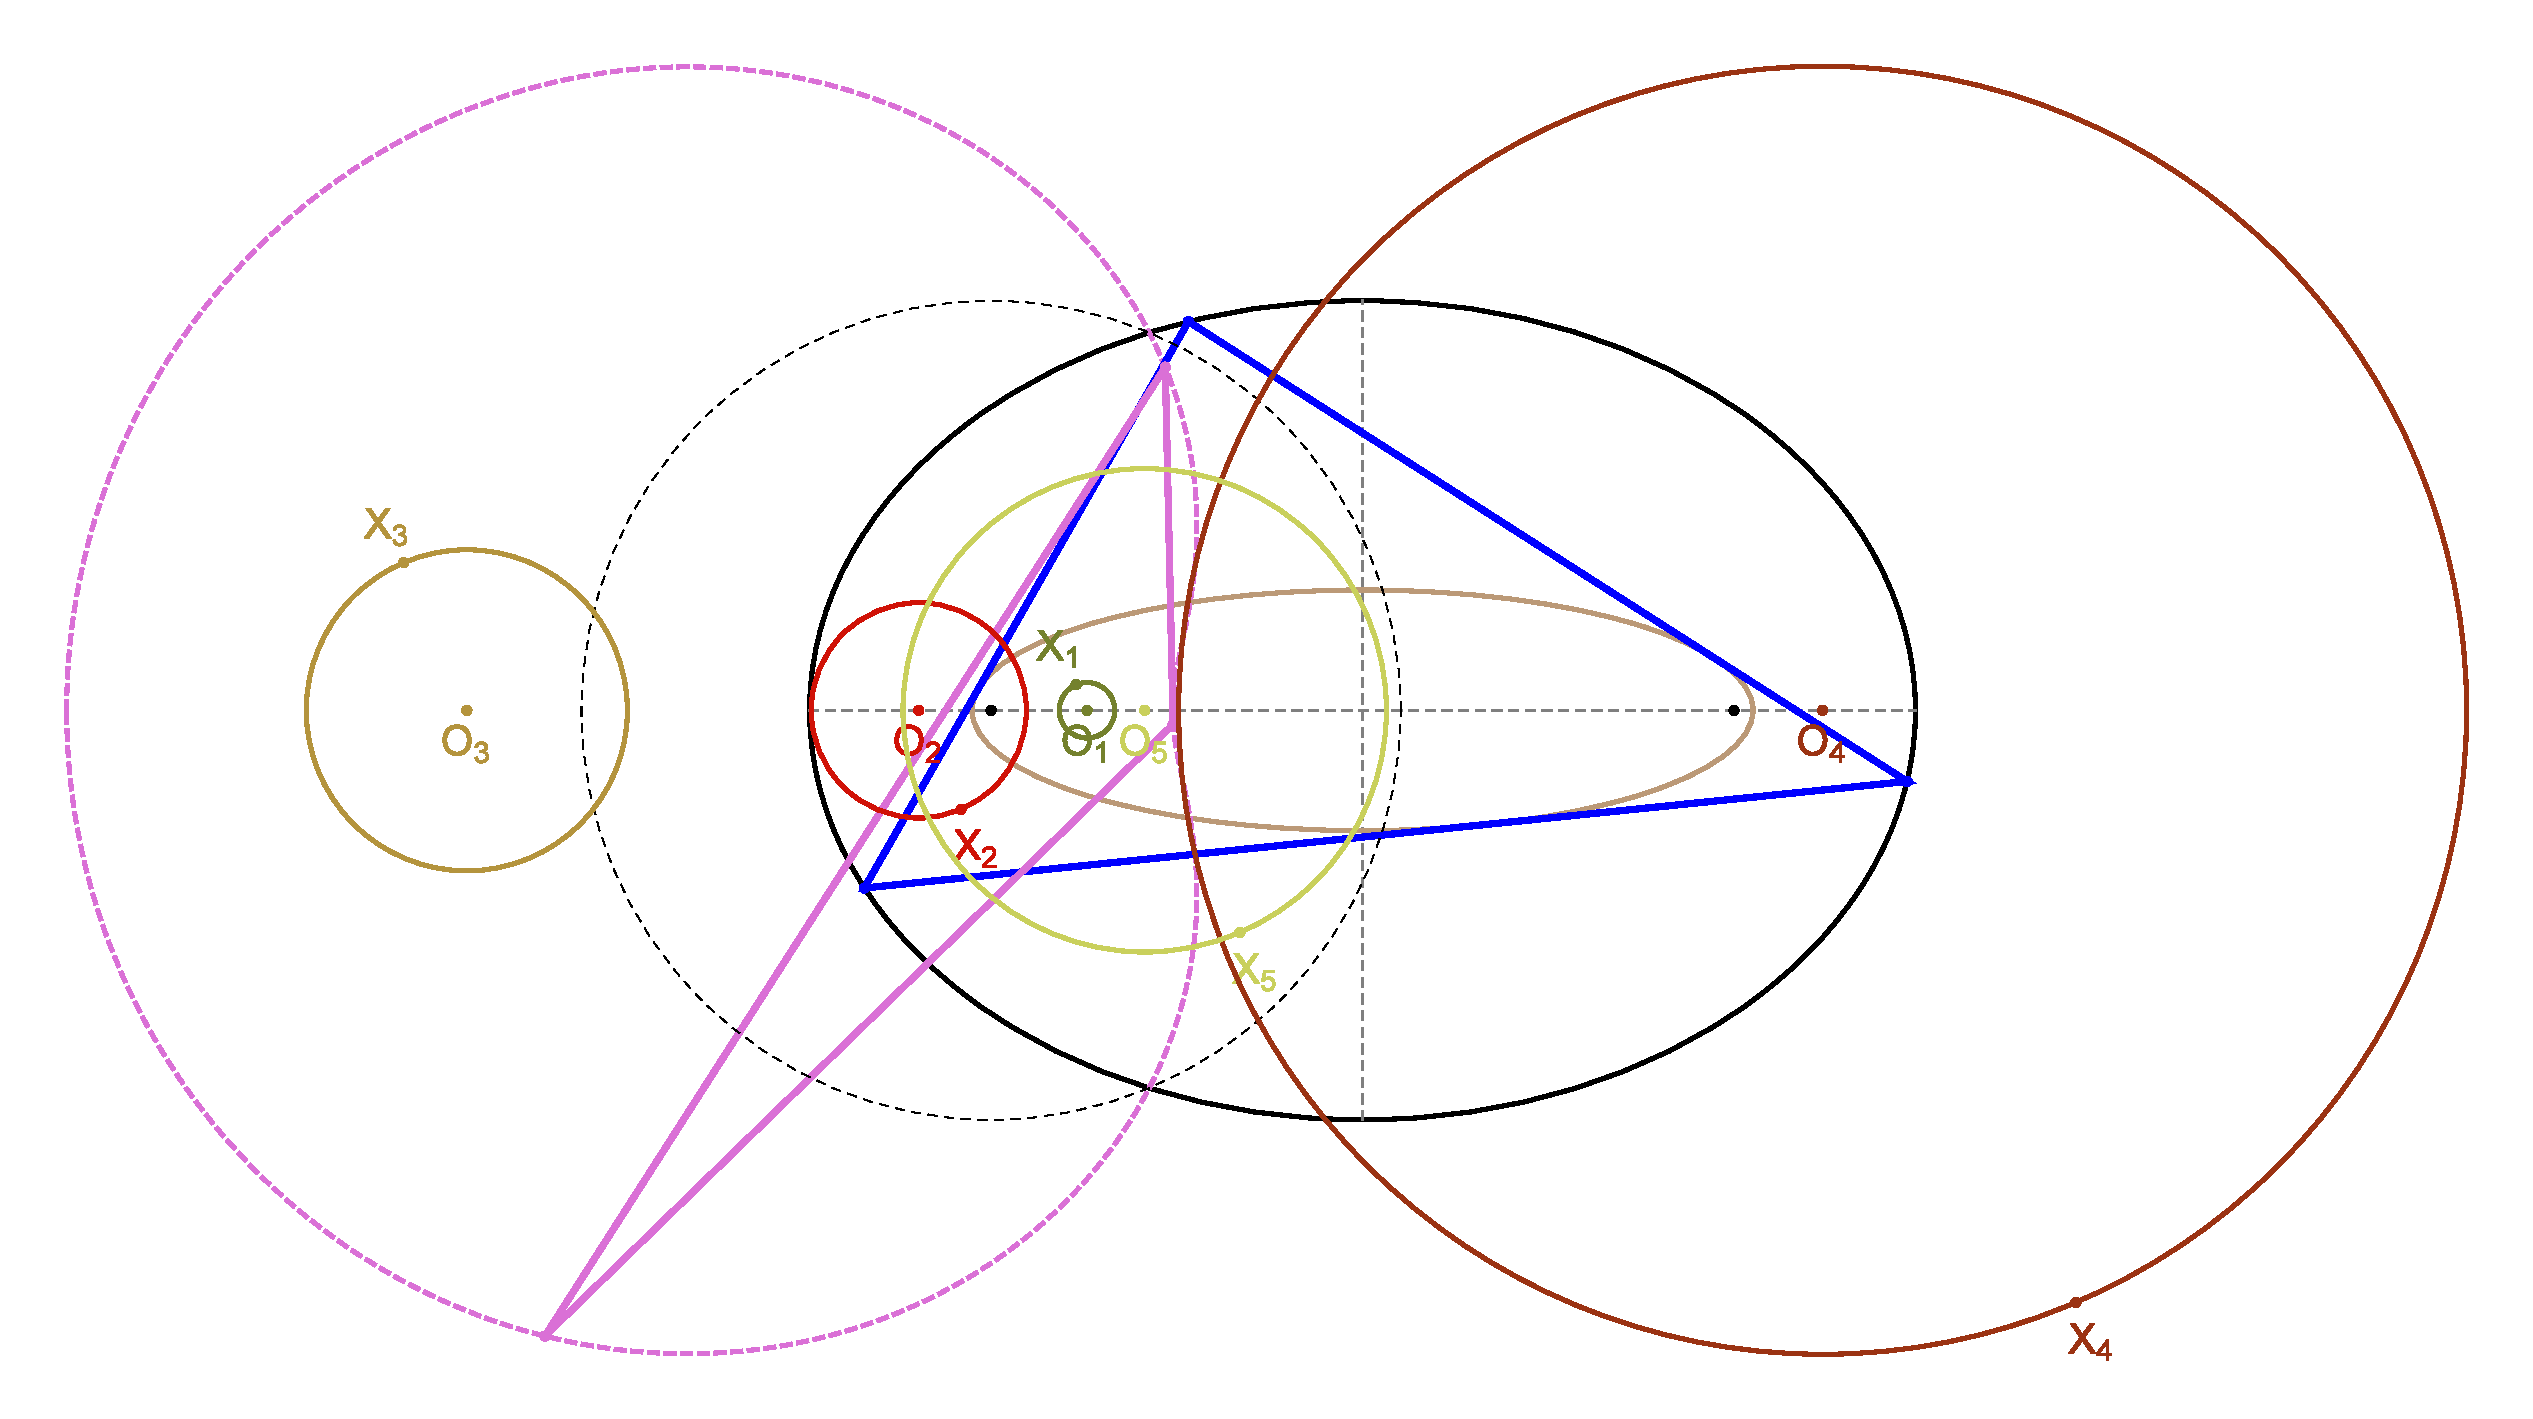
\includegraphics[width=\textwidth]{pics_08_050_n3_inv_loci12345}
    \caption{A focus-inversive 3-periodic (pink) is shown inscribed in Pascal's Limaçon (dashed pink). Also shown are the circular loci of $X_k^\dagger$, $k=1,2,3,4,5$ whose centers $O_i$ all lie on the billiard's major axis. \href{https://youtu.be/OAD2hpCRgCI}{Video}, \href{https://bit.ly/3fW3W1A}{Live}}
    \label{fig:08-n3-loci-12345}
\end{figure}

One remarkable property of focus-inversives is its ability to produce circular loci. Referring to Figure~\ref{fig:08-n3-loci-12345}:

\begin{proposition}
The locus of $X_1^\dagger$ is the circle given by:
\begin{align*}
C_1^\dagger=&\left[c\left(-1+\rho^2\frac{-2a^2+b^2+2\delta}{2b^4}\right), 0\right]\\
R_1^\dagger=&\rho^2\frac{-2\delta^2+b^4+(2a^2-b^2)\delta}{2ab^4}
\end{align*}
\end{proposition}

\begin{proposition}
The locus of $X_2^\dagger$ is the circle given by:

\begin{align*}
C_2^\dagger&=\left[-c\left(1+\rho^2\frac{2a^2-b^2-\delta}{3 a^2 b^2}\right),0\right]\\
R_2^\dagger&=\rho^2\frac{2 a^2-b^2-\delta}{3 a b^2}
\end{align*}
\end{proposition}

\begin{proposition}
The locus of $X_3^\dagger$ is the circle given by:
\begin{align*}
C_3^\dagger=&\left[-c\left(1+\rho^2\frac{a^2+b^2}{2b^4}\right), 0\right]\\
R_3^\dagger=&\rho^2\frac{a(-b^2+\delta)}{2b^4}
\end{align*}
\end{proposition}

\begin{proposition}
The locus of $X_4^\dagger$ is the circle given by:
\begin{align*}
C_4^\dagger=&\left[c\left(-1+\rho^2\frac{(b^2+\delta) \delta}{a^2 b^4}\right), 0\right]\\
R_4^\dagger=&\rho^2\frac{c^2(b^2+\delta)}{a b^4}
\end{align*}
\end{proposition}

\begin{proposition}
The locus of $X_5^\dagger$ is the circle given by:
\begin{align*}
C_5^\dagger=&\left[c\left(-1+ \rho^2\frac{a^4 - 3 a^2 b^2+2 b^4 + 2 b^2 \delta}{4 a^2 b^4}\right), 0\right]\\
R_5^\dagger=&\rho^2\frac{(3a^2-2b^2)b^2+(a^2-2b^2)\delta}{4a b^2}
\end{align*}
\end{proposition}

In \cref{sec:06-loci-types}, 42 triangle centers are identified (from within the first 200 on \cite{etc}), whose loci over billiard 3-periodics are ellipses. Interestingly:

\textcolor{red}{stopped here, need to determine if $X_{190}$ is non-monotonic}

\begin{observation}
Amongst the first 200 triangle centers listed on \cite{etc}, the following triangle centers $X_k^\dagger$ sweep conics over the focus-inversive family:

\begin{itemize}
\item Circles (40): 1,2,3,4,5,8,9,10,11,12,20,21,35,36,40,46,55,56,57,63,65,72,78, 79,80,84,90,100,104,119,140,142,144,145,149,150,153,165,191,200.
\item Ellipses (4): 69,75,85,86.
\item Hyperbolas (3): 47,49,91.
\end{itemize}
\end{observation}

Comparing these with conic locus centers in \cref{sec:06-loci-types}, one realizes that the only ones missing are $X_k$, $k=$88, 162, 190, called ``swans'' in \cref{sec:05-swans}: triangle centers which by construction lie on the $X_9$-centered circumellipse. In particular,  $X_{88}$ and $X_{162}$ were identified as non-monotonic swans, see \cref{sec:05-non-monotonic}. The monotonic swan $X_{100}$ does appear on the list below. Also missing is $X_{190}$, a swan whose monot

Through painstaking CAS-assisted simplification, we were able to obtain compact expressions for only a few of the above circular loci, namely: $X_k,k=$1, 2, 3, 4, 5, 9, 11, 100. 

Referring to Figure~\ref{fig:x159-x934}:

\begin{observation}
Amongst all 29 triangle centers whose loci are ellipses over billiard 3-periodics, only $X_{88}^\dagger$ does not sweep a circular locus over the focus-inversive family. Nevertheless, this locus is algebraic, regular, can be both convex and concave, and is symmetric wrt the major axis of the ellipse.
\end{observation}


\begin{exercise}\label{exer:81}
Show that the ellipse $x^2/a^2+y^2/b^2=1$ and the circle $(x+c)^2+y^2=4a^2$ define  a Poncelet pair such that  all  orbits have   period 3.
\end{exercise}


\begin{exercise}\label{exerc:82} Consider the pair of confocal conics ($\E_1$, $\E_2$, $\H_1$ and $\H_2$) as shown in  \cref{fig:retangulo_exerc82}.

  Consider a ray starting at $F_1$ intersecting the branch $\mathcal{H}_2$ at $P_1$ and  the ray
  $F_2P_1$  intersecting the ellipse $\E_2$  at $P_2$. Analogously, we define the points $P_3=P_2F_1\cap\mathcal{H}_1$, $P_4=P_3F_2\cap\mathcal{E}_1$, $P_5=P_4F_1\cap\mathcal{H}_2$,
  $P_6$, etc.  
  
\noindent i) Determine conditions to obtain $P_5=P_1.$ 
In this case show that the perimeter of the quadrilateral
$P_1P_2P_3P_4$ is constant, i.e., independent of the position of the point $P_1$.  See \cite{dolgirev2014}.


\noindent ii) Analyze the cases when $P_1=\mathcal{E}_2\cap \mathcal{H}_2$ or $P_1=\mathcal{E}_1\cap \mathcal{H}_2$.

 \begin{figure}[H]
 	\begin{center}
 	 \includegraphics[scale=1]{ pics_08_910_dinamica_retangulos.pdf}
 		\caption {Sequence of points $P_1,  \,P_2, \ldots,  P_5 ,  \ldots$  
 		 \label{fig:retangulo_exerc82} }
 	\end{center}
 	\end{figure}
 	
 	\end{exercise}
\section{Research Questions}

\begin{question}
Prove that the locus of $X_{150}^\dagger$ is a circle. Derive center and radius.
\label{que:08-x150}
\end{question}

\begin{question}
Prove that the locus of $X_{934}^\dagger$ is a circle, derive center and radius.
\end{question}

\begin{question}
Prove that the locus of $X_{658}^\dagger$ is an ellipse. Derive its center and semi-axes.
\end{question}

\begin{question}
Prove the loci of $X_k^\dagger$, $k=$69, 75, 85, and 86 are ellipses, derive centers and semi-axes.
\end{question}

\begin{question}
Consider the family of inversive images of excentral 3-periodics with respect to a circle centered at a point $M$ in the plane. Show the symmedian point $X_6$ of such a family will be stationary regardless of $M$. Compute the location of $X_6$. See it in this video \href{https://youtu.be/wwX_QfkjVi0}{Video}.
\end{question}

\chapter{Epilogue: Properties of Pairs of Conics}
\label{chap:09-conics}
%Many insights described in previous chapters were obtained from experimentation and observation of pictures, videos, and interaction with the dynamic geometry of Poncelet configurations. Dozens of notebooks and 100s of small interactive apps were written with \cite{mathematica_v10}. Most of digital artifacts have been assembled in 
\cite{reznik2021-observable-media}.

To further facilitate exploratory discovery of invariants and locus properties of 3-periodic families, we developed a javascript-based locus visualization app \cite{darlan2020-app}.

A typical screenshot of the application is depicted in \cref{fig:09-screenshot}. The dark area is where the animated triangle family is rendered. To its left are ``channel controls'', divided up in four identical areas, which select features to be computed in real time. 

\begin{figure}
    \centering
    \includegraphics[width=\textwidth]{chap_09/pics/pics_09_010_screenshot.png}
    \caption{Locus Visualization app to explore 3-periodic families. Shown are the loci of $X_k$, $k=$1,2,3,4, over billiard 3-periodics. The ``(E)'' suffix indicated they are numerically ellipses. \href{https://bit.ly/3yV8caF}{Live}}
    \label{fig:09-screenshot}
\end{figure}

The most common usage pattern is depicted in \cref{fig:09-flow}, namely: the user selects (i) a triangle family (Poncelet or ellipse-mounted, see below); (ii) the triangle on which computations will be made (the default is ``reference'' but dozens of derived triangles can be chosen); (iii) the locus type, i.e., whether one wishes to trace out a triangle center, a vertex, an envelope, etc., and (iv) which triangle center should the locus be drawn for. The first one thousand triangle centers listed in \cite{etc} are currently supported.

\begin{figure}
    \centering
    \includegraphics[width=\textwidth]{chap_09/pics/pics_09_020_workflow.png}
    \caption{Caption}
    \label{fig:09-flow}
\end{figure}

In the sections below we describe the main functions of the user interface.


\section{Main ellipse and Animation Controls}
\label{sec:09-ellipse-anim}

Before a particular triangle family can be setup and its loci visualized, one must set certain basic animation controls, using the various areas highlighted in \cref{fig:09-animation}. These include (i) the setting of the base ellipse aspect ratio \texttt{a/b} either via typing into the textbox (showing $1.618$ in the picture) or via the scrollbar next to it; (ii) above the animation area, pausing or running the animation and choosing a speed -- slow, medium, or fast. Note: a small ``anim'' dropbox located below the \texttt{a/b} scrollbar, when not in the ``off'' position, triggers a smooth oscillation of the aspect ratio over the range specified in the ``min'' and ``max'' input boxes to its right.

\begin{figure}
    \centering
    \includegraphics[width=\textwidth]{pics_09_130_animation.png}
    \caption{Basic animation controls include (i) the setting of the base ellipse aspect ratio \texttt{a/b} either via typing into the textbox (showing $1.618$ in the picture) or via the scrollbar next to it; (ii) above the animation area, pausing or running the animation and choosing a speed -- slow, medium, or fast. Note: a small ``anim'' dropbox located below the \texttt{a/b} scrollbar, when not in the ``off'' position, triggers a smooth oscillation of the aspect ratio over the range specified in the ``min'' and ``max'' input boxes to its right.}
    \label{fig:09-animation}
\end{figure}

\subsection{Convenience Animation Controls}

If the animation is paused, hitting the up (or right) and down (or left) arrows on the keyboard allows one to carefully step forward or backward over the triangle family.

The mouse wheel allows for the simulation image to be zoomed or unzoomed.

By clicking and dragging into the main animation area one can pan and reposition the image.
\section{Channel Controls}

As shown in \cref{fig:09-four-channels}, four identical groups of ``channel'' controls are positioned to the left of the main animation window. \cref{fig:09-single-channel} zooms in one of them, whose individual settings are explained next.

\begin{figure}
    \centering
    \includegraphics[width=.6\textwidth]{pics_09_030_four_channels.png}
    \caption{Four identical groups of ``channel'' controls positioned to theleft of the main animation window.}
    \label{fig:09-four-channels}
\end{figure}

%\includegraphics[trim=left bottom right top, clip]
\begin{figure}
    \centering
    \includegraphics[trim=0 0 150 0,clip,width=.6\textwidth]{pics_09_040_single_channel.png}
    \caption{Various settings in a single channel control.}
    \label{fig:09-single-channel}
\end{figure}

\section{Choosing a triangle family}

The first step in \cref{fig:09-flow} is the choice of a triangle {\em family}. A specific one is selected 
via the \texttt{mnt} drop-down, see \cref{fig:09-menu-family}. Two types of families are supported: (i) Poncelet, and (ii) ellipse ``mounted'' (see below), which originated the name of the control.

\begin{figure}
    \centering
    \includegraphics[width=.6\textwidth]{pics_09_050_family.png}
    \caption{The \texttt{mnt} drop-down selects a triangle family.}
    \label{fig:09-menu-family}
\end{figure}

\subsection{Poncelet families} Currently we support the following 8 types of 3-periodic Poncelet families interscribed between axis-parallel ellipses, whose names are familiar from previous sections: (i) Confocal (i.e., elliptic billiard), (ii) Homothetic, (iii) with Incircle, (iv) with Circumcircle, (v) Dual, (vi) Excentral (to confocals),  (vii) Poristic, and (viii) the Brocard Porism. Note (i)-(vi),  while the last two are non-concentric.

\subsection{Ellipse ``Mounted''}

Also selectable are triangle families $\T(t)=V_1 V_2 P(t)$, where $V_1,V_2$ are pinned to two points on or near an ellipse, and $P(t)=[a\cos{t},b\sin{t}]$ sweeps the boundary. Let The following fixed locations for $V_1$ and $V_2$ are currently supported:

\begin{enumerate}
    \item \texttt{major}: left and right ellipse vertices (EVs)
    \item \texttt{minor}: top and bottom EVs
    \item \texttt{mixed}: left and top EVs
    \item \texttt{ctrMajor}: center and left EV
    \item \texttt{ctrMinor}: center and top EV 
    \item \texttt{fs}: the 2 foci $f_1$ and $f_2$
    \item \texttt{fsCtr}: center and right focus ($f_2$)
    \item \texttt{fsLeft}: left EV and $f_2$
    \item \texttt{fsRight}: right EV and $f_2$
    \item \texttt{fsTop}: top EV and $f_2$
    \item \texttt{tl-bl}: top left corner of ellipse bounding box (TL) and bottom left of the same (BL)
    \item \texttt{tl-tr}: TL and top right corner (TR) of ellipse bounding box
    \item \texttt{tl-l}: TL and left EV
    \item \texttt{tl-t}: TL and top EV
    \item \texttt{tl-b}: TL and bottom EV
    \item \texttt{tl-o}: TL and center of ellipse
    \item \texttt{tl-br}: TL and center of ellipse
\end{enumerate}

\section{Triangle Type}
\label{sec:09-triangle-type}

The second step in \cref{fig:09-flow} is the choice of the type of triangle with respect to which centers and loci will be computed. This is done the \texttt{tri}  checkbox and drop-down, as shown in \cref{fig:09-menu-triangle}.

\begin{figure}
    \centering
    \includegraphics[width=.6\textwidth]{pics_09_060_triangle.png}
    \caption{The triangle menu selects whether a \texttt{*reference*} or some derived triangle should be used to compute loci. The \texttt{tri} checkbox immediate to the left selects whether the triangle should be drawn or not.}
    \label{fig:09-menu-triangle}
\end{figure}

While the checkbox controls whether selected triangle is drawn or not, the drop-down contains some four-dozen derived triangles. Below the default setting \texttt{*reference*} (this indicates a plain triangle in the family should be used), the choices are organized in three groups:

\begin{enumerate}
    \item Standard ``named'' triangles (undecorated abbreviations), such as \texttt{anticompl} for anticomplementary, \texttt{bci} for BCI triangle, etc., whose construction can be looked up in \cite{mw}.
    \item Exotic triangles (prefixed by a ``.''): \texttt{.andromeda}, \texttt{.antlia}, etc., obtained from \cite{lozada2016-triangles}.
    \item Inversive triangles, e.g., \texttt{*inv-f1*}, \texttt{*inv-f1c*}, etc. (decorated with asterisks). 
\end{enumerate}

Below we document triangles both in the ``standard'' and ``exotic'' groups:

\subsection{Standard Triangles}

These include: Reference, Anticomplementary, BCI, 1st Brocard, 2nd Brocard, 3rd Brocard, 4th Brocard, 5th Brocard, 6th Brocard, 7th Brocard, Circum-Medial, Circum-Mid-arc, Circum-Orthic, Excentral, Extouch, Extangents, Feuerbach, Fuhrmann, Half-Altitude, Hexyl, Incentral, Inner Vecten, Intangents, Intouch, Johnson, Lemoine, Lucas Central, Lucas Inner, Lucas Tangents, MacBeath, Medial, Mixtilinear, 1st Morley Adj, 2nd Morley Adj, 3rd Morley Adj, 1st Neuberg, 2nd Neuberg, Orthic, Outer Vecten, Reflection, Steiner, Symmedial, Tangential, Tangential Mid-Arc, Yff Central, Yff Contact.

\subsection{Exotic Triangles}

These include: Andromeda, Antlia, Apollonius, Apus, Atik, Ayme, Bevan-Antipodal, 1st Circumperp, 2nd Circumperp, Excenters-Incenter Reflections, Excenters-Midpoints, Honsberger, Inverse-in-Excircles, Inverse-in-Incircle, Kosnita, Mandart Excircles, Mandart Incircles, Ursa Major, Ursa Minor. 

\subsection{Inversive Triangles}
\label{sec:09-adv-tri-families}

The options below are images of the reference triangle in a given family under an inversive-like transformation with respect to  unit circle centered on a stationary notable point of the family's underlying ellipse (or caustic), e.g., center, focus, etc.

\begin{itemize}
\item \texttt{*inv-ctr*,*inv-f1*,*inv-f1c*,*inv-f2*}: inversion of vertices with respect to a unit circle centered on the outer ellipse center, outer ellipse left focus, inner ellipse left focus, or outer ellipse right focus, respectively.
\item \texttt{*pol-ctr*,*pol-f1*,*pol-f1c*}: a new, ``polar'' triangle is computed bounded by the polars of the vertices with respect to ellipse center, outer ellipse left focus, or inner ellipse left focus, respectively.
\item \texttt{*ped-lim2*}: this is specific to the confocal family. Computes the pedal triangle with respect to the non-focal limiting point of the bicentric family which is the polar image of the confocal family. 
\item \texttt{*x3map-ctr*,*x3map-f1*,*x3map-f1c*}: consider a triangulation of the original triangle in 3 subtriangles, each of which contains two vertices of the original triangle and either (i) the center of the outer ellipse, (ii) its left focus, or (iii) the inner ellipse left focus, respectively. These transformations compute a new triangle with vertices at the circumcenter of each subtriangle.
\item \texttt{*x3inv-ctr*,*x3inv-f1*,*x3inv-f1c*}: these compute the inverses of the previous transform with respect to the same points.
\item \texttt{*crem-ctr*,*crem-f1*,*crem-f2*}: sends the reference vertices to their images under a quadratic Cremona transformation, which sends $(x,y)\rightarrow(1/x,1/y)$. The origin will be the center of the outer ellipse, its left focus, or its right focus, respectively. 
\end{itemize}

Note: four additional settings \texttt{*inf-x*,*inf-y*,*inf-x2*,*inf-y2*} are provided and are experimental and non-inversive. They dynamically set the $x$ or $y$ coordinate of each vertex so they slide along infinity-like Lissajous curves. 

\section{Locus Type}

The third step in \cref{fig:09-flow} is the choice of type of locus to be drawn, or more precisely, the feature selected from the family/triangle combination previously selected. This is done with the $\mathcal{L}_i$ menu at the top of the control group, $i=1,2,3,4$, shown in \cref{fig:09-menu-locus}.

\begin{figure}
    \centering
    \includegraphics[width=.6\textwidth]{pics_09_070_locus.png}
    \caption{The $\mathcal{L}_i$ menu selects the locus type to (triangle center, vertex, envelope, etc.).}
    \label{fig:09-menu-locus}
\end{figure}

There are three conceptual groups of locus types: (i) triangle centers and vertices, (ii) segment envelopes, and (iii) bicentric pairs. These are explained next.

\subsection{Centers and Vertices}

\begin{enumerate}
\item \texttt{off}: it indicates the trace (locus) of this channel should not be drawn. It is the default setting for channels $2,3,4$ upon startup.
\item \texttt{xn}: draw the locus of the selected triangle center, as in  \cref{sec:09-triangle-center};
\item \texttt{v1}, \texttt{v2}, \texttt{v3}: show the trace of one of thee vertices of the triangle family. In Poncelet families, these will sweep out the same curve, but this is not the case for ellipse-mounted families.
\item \texttt{ort}: the {\em orthopole} of line $X_m X_n$, see \cite[Orthopole]{mw}, where $m$ and $n$ are selected triangle and cevian centers, see \cref{sec:09-triangle-center} and \cref{sec:09-cevian}.
\end{enumerate}

\subsection{Envelopes}

\begin{enumerate}
\item \texttt{env}: the envelope of segment $X_m X_n$, $m{\neq}n$, where $m$ (resp. $n$) is the selected triangle (resp. cevian) center. 
\item \texttt{e12}, \texttt{e23}, \texttt{e31}: the envelope of side $V_i V_j$ of the triangle family. Note these are one and the same (resp. distinct) for Poncelet (ellipse-mounted) families. 
\item \texttt{e1x}, \texttt{e2x}, \texttt{e3x}: the envelope of $V_i X_n$, i.e., the line from a given vertex to a selected triangle center. In a concentric Poncelet family, the envelope of $V_i X_1$ will be the outer ellipse's evolute, see it \href{https://bit.ly/3fNKV2P}{Live}.
\end{enumerate}

\subsection{Bicentric Pairs}

Only a few have so far been implemented, from the copious list in \cite{kimberling2020-bicentric}.

\begin{enumerate}
 \item $\Omega_1,\Omega_2$: the Brocard points
    \item $\beta_1,\beta_2$: the Beltrami points: inversions of the Brocard points with respect to the circumcircle
    \item $\mu_1,\mu_2$: also known as ``Moses'' points: inversion of the Brocard points with respect to the incircle.
    \item $\sigma_1,\sigma_2$: the two foci of the Steiner circumellipse (aka. the Bickart points)
\end{enumerate}

\section{Triangle Center}
\label{sec:09-triangle-center}

The fourth and final step in \cref{fig:09-flow} is the choice of triangle center $X_k$ in the region highlighted in \cref{fig:09-menu-xn}. There are three ways to choose $k\in[1,1000]$: (i) by typing/editing the text field showing $k$, (ii) incrementing or decrementing $k$ by clicking on the ``-'' and ``+'' symbols around the text field; (iii) using the scrollbar to the right of the ``+'' control, to quickly scroll through all 1000 values of $k$. In fact after any of these is performed, this set of controls becomes ``focused'' in such a way that (iv) left (resp. right) arrow keystrokes will decrement (resp. increment) the value, allowing mouse-free traversal of triangle centers.

\begin{figure}
    \centering
    \includegraphics[width=.6\textwidth]{pics_09_080_xn.png}
    \caption{Controls used for the selection of a particular triangle center $X_k$.}
    \label{fig:09-menu-xn}
\end{figure}



\section{Cevians, Pedals, \& Co.}
\label{sec:09-cevian}

An additional ``cevian-like'' transformation with respect to an additional triangle center $X_m$ can be applied to the triangle type selected in \cref{sec:09-triangle-type}. Let us call the latter the ``parent'' triangle.
The specific transformation is selected via the drop-down menu in \cref{fig:09-menu-cevian} (the default setting is \texttt{pn off}, meaning this additional transformation is inactive), and $X_m$ via the numeric input box to the right of the menu.

The $X_m$-transformations possible are grouped into (i) traditional, (ii) inversive, (iv) reflexive, and (iv) triangulated. Below, let $T_m$ denote the transformed triangle, and $P_i$, $i=1,2,3$, the vertices of the parent triangle.

\begin{figure}
    \centering
    \includegraphics[width=.6\textwidth]{pics_09_090_cevian.png}
    \caption{Cevian-like triangles and number box to select a triangle center playing the role of $Q$ (see text).}
    \label{fig:09-menu-cevian}
\end{figure}

\subsection{Traditional}

Available in this groups are the standard constructions for (i) Cevian,  (ii) Anticevian, (iii) Circumcevian, (iv) Pedal, (v) Antipedal, and (vi) Trilinear Polar triangles described in \cite{mw}. Recall that the latter produces a degenerate (segment-like) triangle, see \cite[Trilinear Polar]{mw}.

\subsection{Inversive}

\begin{itemize}
\item \texttt{invert}: $T_m$ will have vertices at inversions of the parent one with respect to a unit circle centered on $X_m$.
\item \texttt{polar}: $T_m$ will be bounded by the polars (infinite lines) of the parent's vertices with respect to a unit circle centered on $X_m$, see \cite[Polar]{mw}.
\item \texttt{inv-excircs}: $T_m$ will have vertices at inversions of $X_m$ with respect to its excircles, see \cite[Excircle]{mw}. 
\item \texttt{polar-exc}: $T_m$ will be bounded by the polars (infinite lines) of $X_m$ with respect to each of the parent's excircles. 
\end{itemize}


\subsection{Reflexive}

\begin{itemize}
\item \texttt{vtx-refl}: $T_m$ has vertices at the reflections of $X_m$ on the parent vertices. 
\item \texttt{side-refl}: $T_m$ has vertices at the reflections of $X_m$ on the sidelines of the parent triangle.
\end{itemize}

\subsection{Triangulated}

Triangulate the parent with respect to $X_m$, i.e., consider the following subtriangles: $T_{23} = X_m P_2 P_3$, $T_{31} = X_m P_3 P_1$, and $T_{12} = X_m P_1 P_2$.

\begin{itemize}
\item \texttt{3-circums}: $T_m$ has vertices at the circumcenters of $T_{23}$, $T_{31}$, and $T_{12}$. 
\item \texttt{3-inv}: The inverse of \texttt{3-circums}. $T_m$ is such that the circumcenters of its three sub-triangles are the vertices of the parent. The vertices of $T_m$ are the non-$X_m$ intersections of a circle through $X_m$ and $P_i$ with a circle through $X_m$ and $P_{i+1}$, cyclically. 
\item $X_k$-map, $k\in[1,11]$: $T_m$ has vertices at the $X_k$ of $T_{23}$, $T_{31}$, and $T_{12}$. Note: $X_3$-map is the same as the \texttt{3-circums} setting.
\end{itemize}

\section{Notable Circles}
\label{sec:09-inversion-circles}

Dozens of circles can be visualized with respect to the triangle family selected in \cref{sec:09-triangle-type}. These are selected via the (left) drop-down menu highlighted in \cref{fig:09-menu-circles}. The \texttt{circs off} setting is the default. The possible choices are organized in two groups: (i) ellipse-affixed, and (ii) central circles.

\begin{figure}
    \centering
    \includegraphics[width=.6\textwidth]{chap_09/pics/pics_09_100_circles_inv.png}
    \caption{The left drop-down selects an ellipse-based circle or a ``central'' circle for both visualization and/or as references for inversive transformations.}
    \label{fig:09-menu-circles}
\end{figure}

\subsection{Ellipse-Affixed Circles}

These are asterisk-decorated to indicate that they refer to a unit circle centered on a notable point of the ellipse (or caustic) used to generate a given triangle family, to be sure:

\begin{itemize}
\item \texttt{*f1*}: the left focus of the outer ellipse. Note: in the poristic (resp. excentral) family this becomes the center of the outer circle (resp. caustic = elliptic billiard).
\item \texttt{*f1c*}: the left focus of the inner ellipse. 
\item \texttt{*f2*}: the right focus of the outer ellipse. Note: in the poristic (resp. excentral) family this becomes the incenter (resp. a focus of the outer ellipse.
\item \texttt{*ctr*}: the center of the system.
\end{itemize}

\subsection{Central Circles}

Most of these are defined in \cite[Central Circles]{mw}:

\begin{itemize}
\item \texttt{adams}: the Adams circle
\item \texttt{appollon1,appollon2,appollon3}: 1st, 2nd, and 3rd Appollonius circles (which intersect on the isodynamic points)
\item \texttt{bevan}: the Bevan circle, circumcircle of the excentral triangle
\item \texttt{brocard,brocard2}: the Brocard circle and the so-called ``2nd'' Brocard circle.
\item \texttt{circum}: the circumcircle
\item \texttt{conway}: Conway's circle
\item \texttt{cosine}: the cosine (or 2nd Lemoine) circle 
\item \texttt{cos.exc}: the cosine circle of the excentral triangle
\item \texttt{ehrmann}: Ehrmann's 3rd Lemoine circle, see \cite{darij2012-ehrmann}.
\item \texttt{excircle1,excircle2,excircle3}: the three excircles
\item \texttt{euler}: Euler's circle
\item \texttt{furhmann}: Furhmann's circle
\item \texttt{gallatly}: Gallatly's circle
\item \texttt{gheorghe}: Gheorghe's circle, see \cite[X(649)]{etc}
\item \texttt{incircle}: Incircle
\item \texttt{lemoine}: 1st Lemoine circle
\item \texttt{lester}: Lester's circle
\item \texttt{mandart}: Mandart's circle
\item \texttt{moses,moses rad}: Moses's circle and Moses' radical circle
\item \texttt{parry}: Parry's circle
\item \texttt{reflection}: the ``reflection'' circle (circumcircle of the reflection triangle)
\item \texttt{schoutte}: Schoutte's circle
\item \texttt{spieker}: Spieker's circle
\item \texttt{taylor}: Taylor's circle
\end{itemize}

As shown in \cref{fig:09-three-circles}, several circles can be shown simultaneously. To do this select one for each channel (maintaining the same triangle family and type), and make sure to check the 

\begin{figure}
    \centering
    \includegraphics[width=.8\textwidth]{pics_09_110_simult_circs.png}
    \caption{The incircle, circumcircle, and Bevan circle are viewer simultaneously, by choosing them on the circle menu in 3 separate channels. Notice that to make the circle appear, one must check the \texttt{tri} checkbox in the lower left of that channel control area. \href{https://bit.ly/3poF5YQ}{Live}}
    \label{fig:09-three-circles}
\end{figure}

\section{Inversive Transformations with respect to a Circle}

Provided a circle $\Cm$ is selected (see above section), one can add an inversive-type transformation with respect to it. This is done via the (right) drop-down menu highlighted in \cref{fig:09-menu-circles}. The possible transformations are as follows: 

\begin{itemize}
    \item \texttt{inv off}: No transformation is performed.
    \item \texttt{inv xn}: invert the selected triangle center (see \cref{sec:09-triangle-center}) with respect to $\Cm$.
    \item \texttt{inv tri}: invert the vertices of triangles in the family with respect to $\Cm$.
    \item \texttt{pol tri}: compute a new triangle bounded by the polars of the original vertices with respect to $\Cm$.
    \item \texttt{cre xn}: send the selected triangle center to its image under a quadratic Cremona transformation (QCT) $(x,y)\rightarrow(1/x,1/y)$, where $(x,y)$ are the coordinated of the center of $\Cm$. 
    \item \texttt{cre tri}: compute a new triangle whose vertices are images of the QCT with respect to the center of $\Cm$.
\end{itemize}

\section{Conic and Invariant Detection}

\subsection{Curve Type}

As shown in \cref{fig:09-conic-invariants}, when one or more loci are displayed, the app  indicates in the lower right-hand side of the corresponding control group, the curve type of the locus (detected via least-squares curve fitting). The following codes are used:

\begin{itemize}
    \item \texttt{X}: non-conic
    \item \texttt{E}: ellipse
    \item \texttt{H}: hyperbola
    \item \texttt{P}: parabola (very rare)
    \item \texttt{L}: line or segment
    \item \texttt{*}: a stationary point.
\end{itemize}

The same code is also appended (in parenthesis) to the (moving) triangle center being displayed, for example, \cref{fig:09-conic-invariants}, \texttt{X2(E),X3(E),X4(E)}, indicate the loci of barycenter, circumcenter, and orthocenter are ellipses over billiard 3-periodics.

\begin{figure}
    \centering
    \includegraphics[width=.8\textwidth]{pics_09_120_conic_invariants.png}
    \caption{An indication as to curve type of each locus appears in a small box in the lower right-hand side of each control group. In the picture, \texttt{X} means the first locus (incenter over the excentral family) is non-conic. An \texttt{E} in the remainder 3 channels indicates their loci are ellipses. Notice the same indicator is appended to the instantenous location of the triangle centers being tracked, e.g., \texttt{X3(E)} indicates the locus of the circumcenter is an ellipse. \href{https://bit.ly/3uXndpa}{Live}}
    \label{fig:09-conic-invariants}
\end{figure}

\subsection{Detection of Metric Invariants}

The app also reports when certain basic, metric quantities are invariant, currently over triangles in the first channel only. These appear as a single line at the bottom of the animation area of a given experiment, see \cref{fig:09-conic-invariants}. In the example, the following line of text is reported:

\[ L=7.14..., r/R=0.32..., \prod\cos'=0.0811, A'/A=6.6... \]

In turn, this means that perimeter $L$ and ratio $r/R$ of inradius-to-circumradius are  numerically invariant over the reference family selected in channel 1, and that the product $\prod\cos'$ of cosines, and ratio $A'/A$ of derived-by-reference areas is constant (these are observations first introduced in \cite{reznik2020-intelligencer}).

Reported invariants appear unprimed to refer to the reference triangle in a given family. Primed quantities will appear when a derived triangle has been selected (e.g., ``excentral''), allowing for mutual comparison. 

The following quantities are currently reported, when numerically invariant:

\begin{itemize}
    \item $L,A$: perimeter and area
    \item $r,R$: inradius and circumradius
    \item $r/R$: ratio of inradius-to-circumradius, tantamount to invariant sum of cosines since $\sum{\cos}=1+r/R$.
    \item $\cot(\omega)$: the cotangent of the Brocard angle
    \item $\sum{s^2},\sum{1/s},\sum{s^{-2}}$: sum of squared, reciprocal, or reciprocal-squared sidelengths, respectively.
    \item $\prod\cos$: the product of internal
    \item $\prod{s}$: the product of sidelengths
    \item $R_c$: if a circle is selected via the circle menu (\cref{sec:09-inversion-circles}), whether its radius is constant.
\end{itemize}

Also reported whenever a derived triangle is selected, are one of $L'/L$, $A'/A$, $A'.A$, $R_c'/R_c$ if these are invariant.
\section{Odds \& Ends}

\subsection{Ellipse, Locus Range, and Animation Background} 

As shown in  \cref{fig:09-ellipse-range}, the area immediately below the four sets channel controls the following parameters:

\begin{itemize}
    \item \texttt{ell} checkbox: whether the main ellipse underlying a triangle family of choice should be drawn or not.
    \item Rotation menu: the default \texttt{rot off} setting leaves the animation window as is. Settings  \texttt{$90^\circ$,$180^\circ$,$270^\circ$} apply a global rotation to the picture drawn.
    \item \texttt{rmax} menu: the (half-side) of the square bounding box where points in all loci are evaluated, respective to the minor semi-axis of the ellipse, assume to be of unit length. Ideally, this should be set to as small a value as able to contain all loci. 
    \item \texttt{bg}: used to set the background color of the main animation window, dark blue by default. By clicking on the colored square an RGB picker window pops-up permitting fine control of the color.
    \item \texttt{invert} button: single-click inversion (in RGB space) of colors of background and loci currently in being drawn.
\end{itemize}

\begin{figure}
    \centering
    \includegraphics[width=.8\textwidth]{pics_09_140_animation_appearance.png}
    \caption{In the highlighted area controls are available to (i) \texttt{ell}: show or hide the main ellipse, (ii) \texttt{rot xxx}: apply a global rotation to the animation widow, (iii) \texttt{rmax}: set the bounding box of the area in which loci are computed, (iv) \texttt{bg}: set the animation window's background color, and (v) \texttt{invert}: invert (RGB negative) colors of background and all loci drawn.}
    \label{fig:09-ellipse-range}
\end{figure}

\subsection{Resetting the UI and Recentering the Animation} 

\cref{fig:09-anim-appearance} highlights \texttt{reset UI} and \texttt{center UI} push-buttons are located at the top-left corner of the app. These are used to (i) restore all controls in the app to their default values, and (ii) recenter the geometry drawn to the center of the animation, respectively. 

\subsection{Setting the Locus Color}

Also shown in \cref{fig:09-anim-appearance} are color and rescaling controls to the right of the triangle center scrollbar. These are permit (i) selection of a color specific to a particular locus being drawn, and (ii) a resizing/re-centering of the particular locus so as to best fit the animation window.

\begin{figure}
    \centering
    \includegraphics[width=.8\textwidth]{pics_09_150_centering_bbox.png}
    \caption{Reset and center push-buttons are located at the top-left corner of the app.  which (i) \texttt{reset UI}: all controls in the app are restored to their default values; (ii) \texttt{center UI}: the center of the simulation is panned back to the center of the animation area. This is useful after having previously panned the picture via a mouse drag. Also shown is (iii) a color selector square located to the right of every triangle center scrollbar, through which a new color can be selected for displaying the corresponding locus. Finally, (iv) a \texttt{bbox} push button is provided to repositing and scale the geometric scene so as to best fit it in the available space.}
    \label{fig:09-anim-appearance}
\end{figure}

\subsection{Collapsing the Locus Control Area}

The ``hamburger'' control shown in \cref{fig:09-hamburger} can be used to hide/expand the set of controls on the left marging of the app, sometimes useful for demonstration purposes.

\begin{figure}
    \centering
    \includegraphics[trim=0 0 150 0,clip,width=.6\textwidth]{pics_09_170_hamburger.png}
    \caption{The hamburger control (three horizontal bars) located to the right of the the main controls can be clicked to hides/expand the main controls.}
    \label{fig:09-hamburger}
\end{figure}
\section{Color-filling loci}

\begin{figure}
    \centering
    \includegraphics[width=.8\textwidth]{pics_09_160_color_fill.png}
    \caption{Color-filling controls.}
    \label{fig:09-color-filling}
\end{figure}

\section{Jukebox Playback}

\section{Sharing and Exporting}

%\section{Examples}

%\section{Truckload?}






\chapter{Conclusion}
\label{chap:10-conclusion}
%\input{chap_10/10_010_main}

\appendix
% \chapter{Triangle Geometry}
\label{app:app-triangle}


\section{Trilinears Coordinates}
\label{app:Atrilins}

The triangle is labeled in the usual (Euler's) manner: vertices $A$, $B$, $C$; angles $A$, $B$, $C$;
and sidelengths $a$, $b$, $c$: $a=|BC|,\; b =|AC|,\; c =|AB|$. If $X$ is a point in the plane of
the triangle $ABC$, then its position is completely determined by the ratios of directed distances (with signal)
from $X$ to the sidelines. Such ratios can therefore serve as coordinates for $X$.
Any ordered triple $[p, q,r]$ of numbers respectively proportional to the
directed distances (with signal) from $X$ to the sidelines $BC$, $CA$, $AB$ are called {\em  homogeneous trilinear coordinates}, or,  {\em  trilinears.}

\begin{figure}
    \centering
  % \includegraphics[scale=0.5]{trilinear.pdf}
 \includegraphics[scale=0.5]{zappA/pics/pics-appA-020-trilinear_signal.pdf}
    \caption{Trilinear coordinates in the plane.}
    \label{fig:trilinear_signal}
\end{figure}

Consider a point given in  homogeneous trilinear coordinates $[p,q,r]$.   Then   $k p,k q$ and $k r$, with
%
\[
k=\frac{2\Delta}{a p+b q+c q}
\]
are the directed distances (with signal) to the sidelines of the triangle $ABC$. This normalization is necessary  to      determine the position of the point in relation to reference triangle $ABC$. Otherwise, is more convenient to consider the homogeneous trilinear coordinates.

The trilinear coordinates of the vertices of a reference triangle are
\[ [\frac{2\Delta}{a},0,0],\;\;B=[ 
0,\frac{
	\Delta}{b} ,0],\;\; C=[
0,0,\frac{2\Delta}{c},0].
\]

The incenter, given by $[1,1,1]$ has equal distance to the sidelines given by $(a+b+c)/2\Delta$ that is equal to the radius of the incircle.


\section{Triangle Centers}
\label{app:Atri-ctrs}

Let $\mathbb{T}$ be the set of all triples $(a, b, c)$ of real numbers that are sidelengths of a triangle $ABC$. That is,
\[
\mathbb{T} = \{ (a, b, c): 0 <a< b + c, 0 <b < c +a, 0 < c < a+ b\}.\]

On any subset $U$ of $\mathbb{T}$, define a center  function as a nonzero function $f(a, b, c)$ such that:

\noindent i) $f$ is homogeneous in $a$, $b$, $c$ (i.e., $f(ta, tb, tc) = t^n f(a, b, c)$   for some non negative integer
$n$,  $t > 0$, and all $(a, b, c) $ in $U$.

\noindent ii) $f$ is  symmetric in $b$ and $c$ (i.e., $f(a, c, b)= f(a, b, c)$
for all $(a, b, c)$ in U. 


A center on $U$ is an equivalence class $[p,q,r]$ of ordered triples
$(p,q,r) $ given by
 \[p= f( a, b, c),\;\; q= f( b, c, a),\; r = f( c, a, b)\]
for some center function $f$ defined on $U$. 

\begin{remark}
 Also, it is useful to express the center functions in terms of the angles of the triangle using the relations of the triangle (law of cosines and sines).
\end{remark}
 
Trilinears coordinates $[p,q,r]$  of a point $X=(x,y) \in \mathbb{R}^2$ can be  converted to cartesians coordinates using \cite{mw}:

\begin{equation}
\label{eqn:appAtrilin-cartesian}
X=\frac{p a A + q b B + r c C}{pa+q b+r c}
\end{equation}
where $A=(x_a,y_a)$, $B=(x_b,y_b)$, $C=(x_c,y_c)$ are the vertices of the triangle $ABC$ expressed in cartesian coordinates.

The conversion of cartesians  to trilinears can be done as follows.

Consider a triangle $T=ABC$ with vertices $A=(x_a,y_a),$ $B=(x_b,y_b)$ and $C=(x_c,y_c)$.

Given a point $P=(x_0,y_0)$ the trilinear coordinates of $P$
is given by
{\small 
\[ \left[ \frac{1}{a}( (C-B)\wedge P+B\wedge C): \frac{1}{b}( (A-C)\wedge P+C\wedge A): \frac{1}{c}( (B-A)\wedge P+A\wedge B)\right] \]}
Here $u\wedge v$ is the area of the oriented parallelogram generated by $u$ and $v$.

\begin{remark}
In this book, also it will  frequently used the notation for a triangle: vertices $A=P_1$, $B=P_2$, $C=P_3$ and sidelengths $a=s_1=|P_2-P_3|$, $b=s_2=|P_1-P_3|$,
$c=s_3=|P_1-P_2|$.
\end{remark}

\begin{remark} \label{rem:baricentro_coord}
Another homogeneous coordinates are the so called {barycentrics}. If the   trilinear coordinates of a point is $[p,q,r]$  then its barycentric coordinates is $[ap,bq,cq]$. Observe that $2ap$ is the oriented area of the triangle $[AXB]$. Analogously, $2bq$ (resp. $2cr$) is the oriented area of the triangle $CXA$ (resp. $BXC$).
\end{remark}

\subsection*{Basic Constructions}

Constructions for a few basic Triangle Centers are shown in \cref{fig:constructions}.

\begin{figure}[H]
    \centering
   \includegraphics[width=\textwidth]{zappA/pics/pics_appA_010_constr.eps}
    \caption{Constructions for Triangle Centers $X_i$, $i=1,2,3,4,5,9,11$, taken from \cite{reznik2020-intelligencer}.}
    \label{fig:constructions}
\end{figure}

\begin{itemize}
    \item The incenter $X_1$ is the intersection of angular bisectors, and center of the incircle (green), a circle tangent to the sides at three {\em intouchpoints} (green dots), its radius is the {\em inradius} $r$.
    \item The barycenter $X_2$ is where lines drawn from the vertices to opposite sides' midpoints meet. Side midpoints define the {\em medial Triangle} (red).
    \item The circumcenter $X_3$ is the intersection of perpendicular bisectors, the center of the {\em circumcircle} (purple) whose radius is the {\em circumradius} $R$.
    \item The orthocenter $X_4$ is where altitudes concur. Their feet define the {\em orthic oriangle} (orange).
    \item $X_5$ is the center of the 9-Point (or Euler) circle (pink): it passes through each side's midpoint, altitude feet, and Euler Points \cite{mw}.
    \item The Feuerbach point $X_{11}$ is the single point of contact between the Incircle and the 9-Point circle.
    \item Given a reference triangle $P_1P_2P_3$ (blue), the {\em excenters} $P_1'P_2'P_3'$ are pairwise intersections of lines through the $P_i$ and perpendicular to the bisectors. This triad defines the {\em excentral triangle} (green).\
    \item The {\em excircles} (dashed green) are centered on the excenters and are touch each side at an {\em extouch point} $e_i,i=1,2,3$.
    \item Lines drawn from each excenter through sides' midpoints (dashed red) concur at the {\em Mittenpunkt} $X_9$.
    \item Also shown (brown) is the triangle's {\em Mandart inellipse}, internally tangent to each side at the $e_i$, and centered on $X_9$.
    %This is identical to the $N=3$ Caustic.
\end{itemize}

\begin{table}[H]
    \centering
    \begin{tabular}{|c|c|c|}
    \hline
         $X_k $& triangle center& $f(a,b,c)$ \\
         \hline
     $X_1 $ & incenter & $ 1$ \\
     \hline
          $X_2 $ & barycenter  & ${1}/{a}$ \\
          \hline
              $X_3$ & circumcenter & $\cos A$ \\
              \hline 
              $ X_4$ & orthocenter & $\sec A$ \\
              \hline   
                $X_5$ & center of Euler's circle & $\cos(B - C)$ \\
              \hline  
                $X_6$ & symmedian & $a$ \\
              \hline  
              $X_9$ & mittenpunkt & $b + c - a$ \\
              \hline
                 $X_{11}$ &Feuerbach point  & $1 - \cos(B - C)$ \\
              \hline
               $X_{15}$ & 1st isodynamic point   & $\sin(A+\frac{\pi}{3})$ \\
              \hline
                $ X_{16} $ & 2nd isodynamic point   & $\sin(A-\frac{\pi}{3})$ \\
              \hline
               $X_{33}$ &  \makecell[cc]{perspector of the orthic\\and intangents triangles}  & $1 +\sec{A}$ \\
            \hline
            %  $X_{88}$ & ss & $1/(b+c-2a)$ \\
         %     \hline
    \end{tabular}
    \caption{Some triangle centers and their first trilinear coordinate expressed as a symmetric function $f(a,b,c)$ on the sidelengths. The complete trilinear vector is given cyclically by $[f(a,b,c),f(b,c,a),f(c,a,b)]$. Note that sometimes these are more concisely expressed as trig functions on the angles $A,B,C$ which can be converted back to $f(a,b,c)$ via the law of sines and/or cosines.}
    \label{tab:Xitrilinear}
\end{table}

\begin{proposition}
The trilinear coordinates of $X_2$ are given by $[1/a,1/b,1/c].$
\end{proposition}

\begin{proof}
Consider a triangle of reference $T=ABC$. The midpoint of the segment $BC$ has trilinear coordinates $[0,1/b,1/c].$
In fact,
\begin{align*}
    [0,\frac{a}{2}\sin C, \frac{a}{2}\sin B] &\equiv[0,\sin C,\sin B]=[0,\sin C,\sin B]\\
    &\equiv[0,\frac{R}{b},\frac{R}{c}]\equiv [0,\frac{1}{b},\frac{1}{c}].
\end{align*} 
Analogously, $[1/a,0,1/c]$ and $[1/a,1/b,0]$ are the trilinear coordinates of the other two midpoints of $ABC.$
Therefore, the medial lines are given by $by-cz=0$, $ax-cz=0$ and $ax-by=0$. The intersection of these lines is the point $[1/a,1/b,1/c].$
\end{proof}

\begin{proposition}
The trilinear coordinates of $X_3$ are given by $[\cos A, \cos B, \cos C].$
\end{proposition}
\begin{proof}
Let $O$ be the center of the circumcirle of $ABC$. Draw a perpendicular line from $P$ to the sideline $BC$.
	
As $PO$ is a perpendicular bisector line, it follows that 
\[ \angle BOP=\frac{1}{2}\angle BOC=\angle BAC=A.\]
Therefore,
\[ \frac{ |BP|}{OP}=\frac{a}{2} \cot A \]

As $a/\sin A=2R$ it follows that

\[\frac{a}{2} \cot A= R\sin A\cot A= R\cos A.\]
Performing the same analysis with the other two vertices the result follows.
\end{proof}


\begin{proposition}
The trilinear coordinates of $X_4$ are given by $[\sec A, \sec B, \sec C].$
\end{proposition}
\begin{proof}
The trilinear coordinates of the altitude feet relative to the  side   $BC$  is given by
$[0,\frac{2\Delta}{a}\cos C,\frac{2\Delta}{a}\cos B]$ $   \equiv  [0, \cos C, \cos B]$.  This follows directly by elementary analysis of the geometry of the triangle.
Analogously,   the other two are given by
$[\cos C, 0, \cos A]$ and $[\cos B,\cos A, 0]$. Therefore, computing the intersection of the straight lines $\cos B y-\cos C z=0$ and $\cos A x-\cos C z=0$ it follows that
$X_4=[\mathrm{sec}{A}, \mathrm{sec}{B},\mathrm{sec}{C}].$
\end{proof}

\begin{proposition}
The trilinear coordinates of $X_9$ are given by $[b+c-a, a+c-b, a+b-c]\equiv [\cot\frac{A}{2}, \cot\frac{B}{2},\cot\frac{C}{2}].$
\end{proposition}
\begin{proof}
Consider the excentral triangle $T'=A'BC'$ of $T$
We have that $X_9$   is the point of concurrence of lines drawn from each excentral point to the midpoint of the corresponding side of $ABC$.
The excentral points have trilinear coordinates $A'=[-1,1,1],$ $B'=[1,-1,1]$ and $C'=[1,1,-1]$. The lines passing through the excentral points and the correspondent midpoints $[0,1/b,1/c]$, $[1/a,0,1/c]$ and $[1/a,1/b,0]$ of the sides of the triangle $T$ are given by
\[ (b - c)x +b y - cz=0, \;\; ax  + ( a - c)y -c z=0,\;\; ax -b y  + (a - b)z=0.\]
Solving the linear system above  it follows that
$[x,y,z]=[b+c-a,a+c-b,a+b-c].$
Also, using the laws of cosine  and sine  it follows that
\begin{align*}
\cot\frac{A}{2}&=\frac{\cos A+1}{\sin A}=\frac{(a + b + c)(b+c-a)R}{abc} =k(b+c-a),\;\; k=\frac{R(a+b+c)}{abc}.
\end{align*}
Analogously, $\cot\frac{B}{2}=k(a+c-b)$ and $\cot\frac{C}{2}=k(a+b-c)$. 
\end{proof}


\begin{proposition} Let $P =[p_1,q_1,r_1]$ and $Q=[p_2,q_2,r_2] $ given in trilinear coordinates with respect to
	a reference triangle $ABC$. Suppose that $ap_i+bq_i+cr_i=2\Delta$, i.e., the trilinear coordinates are the actual distances to the sidelines of the triangle.
	Then the  Euclidean distance  $\rho=|P -Q|$ is given by:
		\[ \rho^2\sin^2 B =(p_1-p_2)^2+(r_1-r_2)^2-2|(p_1-p_2)(r_1-r_2)|\cos B.\]
	
	Also we have 
	\begin{align*}
		  \rho^2\sin^2 A&=(q_1-q_2)^2+(r_1-r_2)^2- 2|(r_1-r_2)(q_1-q_2)|\cos A.\\
		 \rho^2\sin^2 C&=(p_1-p_2)^2+(q_1-q_2)^2- 2|(p_1-p_2)(q_1-q_2)|\cos C.	
		%
	\end{align*}
\label{prop:distancePQ}
	\end{proposition}

\begin{proof}
	Consider the  circle  having $PQ$ as diameter and center $O$.   Draw the segments $PA_1$ and $PC_1$ parallels to the sidelines $AB$ and $BC$. Let $C_1C'$ be also a diameter. See  \cref{fig:distance_tri}.
		\begin{figure}[H]\ 
		\begin{center}
			\includegraphics[scale=0.5]{pics_appA_060_distancia_trilinear.pdf}
			%
			\caption { \label{fig:distance_tri}   Distance between two points $P$ and $Q$.}
		\end{center}
	\end{figure}
By the law of cosines we have that
\[ |A_1-C_1|^2=|P-A_1|^2+|P-C_1|^2-2|P-A_1| \;|P-C_1| \cos \alpha \]

Since $C_1C'$ is a diameter it follows that $\angle A_1PC_1=\angle A_1C'C_1$. Therefore,
\[  |A_1-C_1|=|C-C'| \sin\alpha= |P-Q|\sin\alpha= \rho \sin B.\]
Now, by the construction of $A_1$ and $C_1$, we have that
\[ |P-C_1|= |p_1-p_2|,\;\;\;  |P-A_1|=| r_1-r_2|.\]
	This ends the proof.
\end{proof}

Let \[L=\left| \begin{matrix} q_1&r_1\\
q_2&r_2 \end{matrix} \right|, \;\;M=\left| \begin{matrix} r_1&p_1\\
r_2&p_2 \end{matrix} \right|,\;\; N=\left| \begin{matrix} p_1&q_1\\
p_2&q_2 \end{matrix} \right|   \]

Denote
\[ \{L,M,N\}= L^2+
M^2+N^2-2MN\cos A-2LN\cos B-2LM\cos C. 
\]

\begin{proposition}
	
	\[\rho^2=\frac{R^2 \{L,M,N\}}
	{\Delta^2}.\] 
	\end{proposition}
	
	
\begin{proof} The result follows from algebraic manipulations of the three formulas obtained in \cref{prop:distancePQ}. The details are left to the reader.
\end{proof}

\begin{proposition} Let $lx+my+nz=0$ be a straight line.
	Then the distances of the
	vertices of a reference triangle $ABC$ to this line are:
	
	\[p= \frac{2\Delta}{a}\frac{l}{\{l,m,n\}},\;\;
	%
	q=\frac{2\Delta}{b}\frac{m}{
		\{l,m,n\}},\;\;
 r=\frac{2\Delta}{c }\frac{n}{
 \{l,m,n\}}.\]
 
	
\end{proposition}



Two rays $CP$ and $CP'$ are called {\em  isogonal } relative to $C$ when $\angle ACP=\angle BCP'$. Equivalently, the ray $CX_1$ is a the common bisector of $P'CP$ and $ACB$.
If the analogous rays $AP$ and $AP'$ are isogonal ($\angle BAP=\angle BAP'$) we say that the points $P$ and $P'$ are {\em isogonal conjugates}. It can be shown that    
$\angle PBC=\angle P'BC$. 

\begin{proposition} Let  $P$ and $P'$ be isogonal conjugates. If $P=[p,q,r]$ then $P'=[1/p,1/q,1/r]=[qr,pr,pq]$. The map $\varphi(P)= P'$ is an involution, i.e., $\varphi^2=id$.
\end{proposition}

\begin{proof}
 
\end{proof}

\begin{proposition} Consider a triangle $T=ABC$. The points $X_3$ (circumcenter $O$) and $X_4$ (orthocenter $H$)  of $T$ are  isogonal conjugates.  
\end{proposition}

\begin{proof} 
	Consider the triangle $ABC$ and the circumcircle centered at $O=X_3$. The isosceles triangle $BOC$ has  angle $2A$ (or $2\pi-2A) $ at the vertex $O$. Therefore the angle between the ray $CO$ and the segment $BC$ is equal to $\pi/2-A$ (or $A-\pi/2$ ). The  angle between the ray $CX_4$ and the segment $CA$ is $\pi/2-A$ (or $A-\pi/2$ ). Therefore, $X_4=H$ and $X_3=O$ are isogonal relative to $C$. The same conclusion follows for the other vertices. 
		\begin{figure}[H]\ 
		\begin{center}
		 \includegraphics[scale=0.5]{pics_appA_080_isogonalX3X4.pdf}
			\caption { \label{fig:X3X4}   Isogonal conjugate points $X_3$ and $X_4$.}
		\end{center}
	\end{figure}
\end{proof}


\section{Euler Line}

The Euler is a line passing through the pair of isogonal conjugate points $X_3$ and $X_4$.

The equation of Euler line in trilinear coordinates is given by

\begin{align*}
	 \left| \begin{matrix} x& y & z\\
	 	\cos A &\cos B &\cos C\\
	 	\frac{1}{\cos A}& \frac{1}{\cos B}& \frac{1}{\cos C} \end{matrix}
	 \right|=0,\; \\
%	 
\end{align*}
Developing the calculations it follows that the Euler line is given by:

\[  \cos A   (  \cos ^  {2}B - \cos^{2}C
) x+\cos B \left( \cos ^{2} C  -\cos^2 A 
\right) y+\cos C \left(   \cos  ^{2}A-  \cos ^2 B   \right) z=0.\]

In terms of the sides $a$, $b$ and $c$, the Euler line is given by:
\[a(c^2 - b^2) (-a^2 + b^2 + c^2)x + b(a^2 - c^2) (a^2 - b^2 + c^2)y + c(b^2 - a^2) (a^2 + b^2 - c^2)z=0
\]
The point at infinity in the Euler line is the intersection of the Euler line with the line  $ax+by+cz=0$ ( or equivalently 
$\sin A \;x+\sin B\; y+\sin C \; z=0$).

A notable point in the Euler line is the barycenter $X_2$,  which has trilinear coordinates
$[1/a,1/b,1/c]\equiv [\sin A, \sin B, \sin C]$. 



\begin{proposition}\label{prop:circumcircle_tri} Let $T=ABC$ be a triangle.
	The circumcircle in trilinear coordinates is given by
	\[a y z+b x z+c x y=0.\]
\end{proposition}

\begin{proof}
	
	\end{proof}
	
	\begin{proposition}
	    Consider the triangle $A=[\alpha,\beta]$, $B=[-1,0], C=[1,0]$.
	    The Euler line is given by:
	   \[ (3-3\alpha^2 - \beta^2  )x - 2\alpha \beta y + \alpha(\alpha^2 + \beta^2 - 1)=0\]
	\end{proposition}
	
	\begin{proof} In cartesian coordinates:
	\[ X_3=[0, \frac{\alpha^2 + \beta^2 - 1}{2\beta}],\;\; X_4=[\alpha, \frac{1-\alpha^2  }{\beta}]
	\]
	 Therefore the result follows from direct calculations.   
	\end{proof}
	


A {\em derived triangle} $T'$ is constructed from the vertices of  a reference triangle $T$. A convenient representation is by a $3\times  3$  matrix, where each row, taken as trilinears, is a vertex of $T'$.

\subsection{Excentral, medial, and intouch triangles}

The {\em  excentral triangle} is the triangle defined by the intersections of the external bisectors of a triangle.

\noindent The {\em medial triangle} is the triangle whose vertices are the midpoints of the vertices of the reference triangle.

\noindent The {\em intouch triangle}  is the triangle whose vertices are the points of tangency of the  incircle centered at $X_1$(incenter) and the sidelines of the reference triangle.



The matrix vertex are given by \cite{mw}: 

%, built from Triangle Center functions $h_1,h_2,h_3$ as follows \cite{kimberling1993_rocky}:

%\begin{align*}
%T'=
%\left[
%\begin{matrix}
%h_1(s_1,s_2,s_3) & h_2(s_1,s_2,s_3) & %h_3(s_1,s_2,s_3)\\ 
%   h_3(s_2,s_3,s_1) & h_1(s_2,s_3,s_1) & %h_2(s_2,s_3,s_1) \\
%   h_2(s_3,s_1,s_2) & h_3(s_3,s_1,s_2) & %h_1(s_3,s_1,s_2)
%\end{matrix}
%\right]
%\end{align*}

\begin{equation*}
\left[
\begin{matrix}
-1&1&1\\1&-1&1\\1&1&-1
\end{matrix}
\right],\;
\left[
\begin{matrix}
0&b^{-1}&c^{-1}\\a^{-1}&0&c^{-1}\\a^{-1}&b^{-1}&0
\end{matrix}
\right],\;
\left[
\begin{matrix}
0&\frac{a c}{a-b+c}&\frac{a b}{a+b-c}\\
\frac{b c}{ b+c-a}&0&\frac{a b}{a+b-c}\\
\frac{b c}{ b+c-a}&\frac{a c}{a-b+c}&0
\end{matrix}
\right]
\end{equation*}

 \subsection{Brocard triangle}
 
 The first Brocard point (resp. second Brocard point)  of a triangle $T=ABC$ (labelled in counterclockwise order) is the unique interior point $\Omega$ such that the angles $\angle\Omega AB$,   $\angle\Omega BC$ and  $\angle\Omega CA$  are equal (resp. the point $\Omega'$ such that the three angles $\angle\Omega' BA$,   $\angle\Omega' CB$ and  $\angle\Omega' AC$ are equal).
 
 The trilinear coordinates of $\Omega$ is $[c/b:a/c:b/a].$ And, the trilinear coordinates of $\Omega'$ is $[b/c:c/a:a/b].$
 
 \begin{figure}[H]
 %   \centering
  % \includegraphics[scale=0.5]{trilinear.pdf}
      \includegraphics[scale=0.4]{pics_appA_030_brocard_points.pdf}
    \caption{Brocard points $\Omega$ and $\Omega'$ of a triangle $ABC$.}
    \label{fig:brocard_points}
\end{figure}

Consider the six straight lines passing through the vertices $A,B,C$ and the Brocard points $\Omega$ and $\Omega$.

The triangle with vertices $B_1=A\Omega\cap B\Omega'$, $B_2=C\Omega\cap A\Omega'$ and $B_3=B\Omega\cap C\Omega'$ is called the {\em first Brocard triangle}. See \cref{fig:brocard_triangle}.
 \begin{figure}[H]
    \centering
  % \includegraphics[scale=0.5]{trilinear.pdf}
\includegraphics[scale=0.6]{pics_appA_040_brocard_triangle.pdf}
    \caption{Brocard triangle $B_1B_2B_3$ .}
    \label{fig:brocard_triangle}
\end{figure}
The Brocard circle $\mathcal{C}_B$ is the circle passing through the two Brocard points and the $X_3$ (center of the circumcircle of the triangle $ABC$.)
The center of $\mathcal{C}_B$ is  $X_{182}$, which is the middle point of  
the point $X_6$ (symmedian) and $X_{3}.$

The lines $X_3X_6$ and $\Omega\Omega'$ are orthogonal.

Some facts about Brocard points are the following ones. See \cite{johnson29}.

\[ \cot A+\cot B+\cot C=\cot \omega.\]

\[ |\Omega-X_3|=|\Omega'-X_3|=R\sqrt{1-4\sin^2\omega}.\]

\[R_B=\frac{R\sqrt{1-4\sin^2\omega}}{2\cos\omega}.\]

The trilinear vertex matrix of the Brocard triangle $B_1B_2B_3$ is given by:

\begin{align*}
   \left(\begin{matrix} abc& c^3& b^3\\
   c^3&abc & a^3\\
   b^3 &a^3 &abc\end{matrix}\right)
\end{align*}

\subsection{Pedal and Antipedal Triangles}

Given a triangle $T=ABC$  and a point $P$ which is not a vertex of $T$ drop three perpendiculars to the sidelines of $T$. The intersections of theses lines with the sidelines define a triangle $T'=A'B'C'$ that is known as the {\em pedal triangle} of $P$. See \cref{fig:pedal_triangle}, left.

The antipedal triangle is defined by the following construction.
Drop half lines from $P$ to the vertices of the triangle $T$. For each vertex draw a line perpendicular to the correspondent half  line. The intersections of these  lines will be the vertices of the {\em antipedal triangle}. See \cref{fig:pedal_triangle}, right.
 \begin{figure}[H]
    %\centering
  % \includegraphics[scale=0.5]{trilinear.pdf}
      \includegraphics[scale=0.6]{pics_appA_050_pedal_antipedal_triangle.pdf}
    \caption{Pedal triangle $A'B'C'$ of the point $P$.}
    \label{fig:pedal_triangle}
\end{figure}

Let $P=[p:q:r]$ given in trilinear coordinates. The trilinear vertex matrix of the pedal triangle $T'=A'B'C'$ is given by \cite{mw}:

\begin{align*}
   \left(\begin{matrix} 0& q+p\cos C& r+p\cos B\\
   p+q\cos C &0 & r+q\cos A\\
   p+r\cos B & q+r\cos A &0\end{matrix}\right)
\end{align*}


The trilinear vertex matrix of the antipedal triangle $T''=A''B''C''$ is given by \cite{mw}:
 
\begin{align*}
   \left(\begin{matrix} - \frac{ q + p \cos C}{r + p \cos B}& \frac{r + p \cos B}{p + q \cos C}& \frac{q + p \cos C}{p + r \cos B}\\
    \frac{ (r + q \cos A)}{q + p \cos C}& -\frac{r + q \cos A}{p + q \cos  C}& \frac{q + p \cos C}{q + r \cos A}\\
   \frac{q + r \cos A}{r + p \cos B}&\frac{ p + r \cos B}{r + q \cos A} & - \frac{p + r \cos B}{q + r \cos A}\end{matrix}\right)
\end{align*}

 The pedal triangle associated to  $P=X_4$ (orthocenter) is called the {\em orthic triangle}.
 
 For $P=X_1$ (resp. $X_3$) the pedal is the intouch triangle (resp. medial triangle). 
 
 The antipedal of $X_1$ is the excentral triangle.

The notion of pedal triangle  can be generalized for any polygon. From $P$ drop perpendicular half lines to the sidelines (extended) of the polygon. The intersections are the vertices of the {\em pedal polygon.}

Also the {\em  antipedal polygon} is defined analogously to the antipedal triangle.
 
 \subsection{ Anticomplementary triangle}
 
 The anticomplementary triangle of a triangle $T=ABC$ is the triangle $T'=A'BC'$ such that $T$ is the medial triangle of $T$.
 
  \begin{figure}[H]
     \centering
      \includegraphics[scale=0.6]{zappA/pics/pics_appA_0100_anticimplementary.pdf}
    \caption{Anticomplementary triangle $A'B'C'$ of $ABC$.}
    \label{fig:pedal_triangle}
\end{figure}
The center of the circumcircle of $T'$ coincides with the orthocenter of $T$, i.e., $X'_3=X_4$.

The trilinear vertex matrix of the antipedal triangle $T'=A'B'C'$ is given by \cite{mw}:
 
\begin{align*}
   \left(\begin{matrix}-\frac{1}{a} &\frac{1}{b} &\frac{1}{c}\\
    \frac{1}{a} &-\frac{1}{b} &\frac{1}{c}\\
    \frac{1}{a} &\frac{1}{b} &-\frac{1}{c}\end{matrix}\right)
    \end{align*}
   



\section{Inconic and Circumconic of a triangle}
\label{app:A-inconic}

Two triangles $T=ABC$ and $T_1=A_1B_1C_1$ are called in perspective when  the three lines $AA_1$, $BB_1$ and $CC_1$ are concurrent. This point is called the perspector of the pair $\{T,T_1\}$.

Also, the perspective axis of a pair of triangles is the line passing through the   three points of intersection of the correspondent sidelines $AB\cap A_1B_1$,
$AC\cap A_1C_1$ and $BC\cap B_1C_1$.
See \cref{fig:appA-perspector}.

\begin{figure}
    \centering
    %[trim=left bottom right top, clip]
    \includegraphics[trim=0 0 0 30, clip,width=.8\textwidth]{zappA/pics/pics-appA-101-perspector.pdf}
    \caption{Perspector and perspective axis of a pair of triangles $ABC$ and $A_1B_1C_1$.}
    \label{fig:appA-perspector}
\end{figure}

Given a triangle $T=ABC$ and a conic $\E$ the polar triangle of $T$ with respect to $\E$ is the triangle whose sidelines are the polar lines of the vertices   $A,B,C$. See \cref{fig:appA-polar-triangle}
\begin{figure}
    \centering
    \includegraphics[trim=0 0 0 60, clip,width=.8\textwidth]{zappA/pics/pics-appA-150-perspector-triangle-ellipse.pdf}
    \caption{Polar triangle $A_1B_1C_1$ and perspector $X$.}
    \label{fig:appA-polar-triangle}
\end{figure}

A conic $\E$ that is tangent to the sidelines of a triangle $ABC$ is called {\em inconic}. The perspector of the triangles $ABC$ and its polar with respect to $\E$ is called the perspector of the inconic.

In trilinear coordinates, an inconic is of the form:

\[p^2 x^2+q^2 y^2 +r^2 z^2 - 2 q r y z -2 p r x z- 2 p q  x y=0\]
 
 The center of the inconic is given by 
 \[ [c q + b r : a r + c p : b p + a q] \]
 
 The perspector is 
 \[ [\frac{1}{p},\frac{1}{q},\frac{1}{r}] \]


 \begin{remark}
 The Brocard inellipse of a triangle $T=ABC$ is the inconic with parameters $[p,q,r]=[ 1/a,1/b,1/c]$.
 \[ a^2 b^2 z^2 - 2 a^2 b c y z + a^2 c^2 y^2 - 2 a b^2 c x z - 2 a b c^2 x y + b^2 c^2 x^2=0\]
 The center is $X_{39}=[a(b^2 + c^2), b(a^2  +  c^2), c( a^2  + b^2)]$ 
  and their perpesctor is $X_6=[a,b,c]$.
 \end{remark}
 
In   an elliptic  billiard having  3-periodic orbits the perspector of the caustic is the triangular center $X_8$. 
\textcolor{red}{corrigir acima}
The perspector of the billiard is $X_1$. See \cref{fig:appA-X8-X1-perspectors}.
\begin{figure}
    \centering
    %\includegraphics[trim=left bot right top,clip,width=.6\textwidth,frame]
    \includegraphics[trim=80 20 100 15, clip,width=.6\textwidth]{zappA/pics/pics-appA-170-inconic-billiardggb.pdf}
    \caption{Perspectors of the caustic $\E_c$ is $X_8$, and of the billiard $\E$ is the $X_1$ (incenter). }
    \label{fig:appA-X8-X1-perspectors}
\end{figure}

Given a triangle $T=ABC$ the conic passing through the vertices is called {\em circumconic}. The circumconic is unique when the center is fixed; otherwise we have a 2d family of circumconics circumscribing a given triangle. 

In trilinear coordinates the circumconic is of the form
\[ \frac{p}{x}+\frac{q}{y}+\frac{r}{z}=0\]

 The center of the circumconic is given by 

 \[ [p (-a p u + b q + c r), q  (a p - b q + c r),   r (a p + b q - cr)] \]
 
 The perspector of the circumconic (considered as an inconic of the excentral triangle)  is the point $[p,q,r]$.
 
\section{Isogonal and isotomic conjugation}
	
Consider a triangle $T=ABC$ and a point $P$. Denote by $A_1$, $B_1$ and $C_1$ the contact points of the sidelines of $T$ with the incircle. Consider the reflection of the line $AP$ with respect to $AA_1$ and repeat this process for the other two lines, i.e., reflect the line $BP$ (resp. $PC$) with respect to the bisector $BB_1$ (resp. $CC_1$).

The intersection of these three reflected lines is called the {\em isogonal conjugate} of $P$. 
	
Analogously, when we consider reflection of points  with respect to midpoints   we obtain the so called {\em isotomic conjugate} of $P$. More precisely, consider the intersection $A_1$ of the line $AP$ with the sideline $BC$. Reflect $A_1$ with respect to the midpoint $A_m$ of the side $BC$ obtaining the point $A_1'$. Repeat for the other two sides obtaining the points $B_1'$ and $C_1'$. The intersection of the three lines $AA_1'$, $BB_1'$ and $CC_1'$ is the isotomic conjugate of $P$.
	
\begin{figure}
\centering
	    \includegraphics[scale=0.35]{zappA/pics/pics-appA_180-isogonal.pdf}
	     \includegraphics[scale=0.4]{zappA/pics/pics-appA_190-isotomic.pdf}
	    \caption{Isogonal and isotomic conjugatation.}
	    \label{fig:appA-isotomic-isogonal}
	\end{figure}

	 \begin{remark}
 The concept of reflection used here is that of projective geometry. This means that the cross-ratio of the four aligned points, say $A=( a,0,1)$, $B=(b,0,1)$, $C=(c,0,1)$ and $D=(d,0,1)$ is given by:
 \[ [A,B,C,D]=\frac{(c-a)(d-b)}{(d-a)(c-b)}\]
 \end{remark}
	\begin{proposition}
	Let $P=[p,q,r]$ given in trilinear coordinates. Then the isogonal conjugate of $P$ is $[1/p,1/q,1/r]$.
	\end{proposition}
	
	\begin{proof} In trilinear coordinates. Let $P=[p,q,r]$, $A=[1,0,0]$, $B=[0,1,0] $ and $C=[0,0,1]$.
	Then $A_1=[0,1,1]$, $B_1=[1,0,1]$ and $C_1=[1,0,0]$. The line $AP$ is given by
	$q z - r y=0$ and their reflection in relation to the bisector $z=y$ is the line $  q y-r z=0$. Analogously, the other two reflected lines are given by $ x p-r z=0$ and $p x-q y=0$. The intersection of these three lines is 
	\[ [\frac{r z}{p},\frac{r z}{q},\frac{r z}{r}]= [\frac{1}{p},\frac{1}{q},\frac{1}{r}]\]
	\end{proof}

	 
	
		\begin{proposition}
	Let $P=[p,q,r]$ given in trilinear coordinates. Then the isotomic  conjugate of $P$ is $[1/(a^2 p),1/(b^2 q),1/(c^2 r)]$.
	When $P=[p,q,r]_b$ is given in barycentric coordinates   the isotomic conjugate of $P$ is simply $[1/p, 1/q, 1/r]_b$.
	\end{proposition}
 \begin{proof}
 In trilinear coordinates,  let $P=[p,q,r]$, $A=[1,0,0]$, $B=[0,1,0] $ and $C=[0,0,1]$.
	Then the midpoint of the side $BC$ is $A_m=[0,c,b]$. Also, $B_m=[c,0,a]$ and $C_m=[b,a,0]$. The line $AP$ is given by
	$q z - r y=0$. Therefore $A_1=[0,q,r]$ and $A_1'=[0,c^2r,b^2q]$. 
 
	Analogously, the   line $BP$ is given by $   r x-p z=0  $. Therefore $B_1=[ p,0,r]$ and
	$B_1'=[r^ 2c,0,a^2p]$.  
	Therefore the intersection of the   lines $AA_1'$ and $BB_1'$ is the point
	\[[\frac{1}{  a^2 p},\frac{1}{b^2 q},\frac{1}{c^2 r} ] \]
 \end{proof}
 
	\begin{remark}
	Under isogonal conjugation it follows that
	\[\angle P A B = \angle C A I_g(P),\;\; \angle P B C = \angle A B I_g(P),\;\; \angle P C A = \angle B  C I_g(P)\]
	\end{remark}
	The isogonal conjugation is the map $I_g([p,q,r])=[1/p,1/q,1/r]=[q r,p r,p q]$ which is an involution $(I_g\circ I_g=id)$.
	
	The isomotic conjugation is the map $I_m([p,q,r])=[1/(a^2p),1/(b^2 q),1/(c^2r)]=[  q r/a^2, p r/b^2, p q/c^2]$ which is also an involution.

	\begin{proposition} The image of the Euler line by $I_g$ is the circumconic (hyperbola) given by
	
	\begin{align*}
\mathcal{I}_E(x,y,z)&=-c \left( a^2-b^2 \right)   \left( {a}^{2}+{b}^{2}-{c}^
{2} \right) x y+b \left( a^2-c^2 \right)    \left( {a}^{2
}-{b}^{2}+{c}^{2} \right) x z\\
&+a \left( b^2-c^2 \right)  
 \left( {a}^{2}-{b}^{2}-{c}^{2} \right) y z  =0
	\end{align*}
	More general, the image of any line by $I_g$ is a  circumconic.
	\end{proposition}
	
	\begin{proof} Write the Euler line in the parametric form $E(u)=(1-u)X_3+uX_4$ and compute $I_g(E(u))$. Now, writing in the implicit form, it is straightforward to obtain the result stated.
	\end{proof}
	
		\begin{proposition} The image of the Euler line by $I_m$ is circumconic (hyperbola)  by:
	
	\begin{align*}
\mathcal{I}_H(x,y,z)&= a b (a^2 - b^2) (a^2 + b^2 - c^2) x y - a c (a^2 - c^2) (a^2 - b^2 + c^2) x z \\
&- b c (b^2 - c^2) (a^2 - b^2 - c^2)y z=0
	\end{align*}
	
	\end{proposition}
	
	\begin{proof}
	Left to the reader.
	\end{proof}
	
	\begin{proposition} A   billiard  having a triangle $T=ABC$ as 3-periodic orbit is the isogonal conjugate of the antiorthic axis of $T$.
 \label{prop:appA-billiard-antiorthic}
	\end{proposition}
	\textcolor{red}{checar calculo da prova}
	\begin{proof}
	Recall that the antiorthic axis  is the perspective axis of the T and its excentral triangle, and that the elliptic billiard is centered at $X_9$ (mittenpunkt) and its perspector is   $X_1$ (incenter).
	Therefore, it follows that the antiorthic axis is given by $x+y+z=0$.
The elliptic billiard is $xy+xz+yz=0$.
	\end{proof}
	
	\begin{proposition}
Consider a triangle $T=ABC$. Then, in barycentric coordinates we have the following.

\noindent i) If the  circumconic has centre $U=[p,q,r]_b$, then it has perspector $G(U)$, where:
G(U) is the X(2)-Ceva conjugate  
\[ G(u,v,w) = [u.(v+w-u), v.(w+u-v), w.(u+v-w)]\]
%// [u(v+w-u)]
%G(b1,b2,b3) = [b1.(b2+b3-b1), b2.(b3+b1-b2), b3.(b1+b2-b3)]
%[1/b1,1/b2,1/b3]
%Anticomplement: A(b1,b2,b3) = [b2+b3-b1, b3+b1-b2, b1+b2-b3]
\noindent ii) If the  inconic has centre $U$, then it has perspector $T(A(U))$, where
Isotomic: $T(u,v,w) = [1/u,1/v,1/w]$
Anticomplement: $A(u,v,w) = [v+w-u, w+u-v, u+v-w]$
		\end{proposition}
		
		\begin{proof}
		
		\end{proof}
%\textcolor{red}{ver que coordenada usa na observacao abaixo}
%	\begin{remark}
%	A circumconic with center $[x_0,y_0,z_0]$ is given by
%	\[(x_0-y_0-z_0) y z+(y_0-x_0-z_0) x z+ (z_0-x_0-y_0) xy=0\]
%	In the billiard the center is $X_9=[b + c - a , c + a - b , a + b - c]$.
%	
%	\end{remark} 


\begin{exercise}\label{ex:1chap1}
Let $P=[p:q:r] $ be an interior point of an equilateral triangle $T=ABC$.

\noindent i) Show that the distances of $P$ to the sidelines of the triangle $T$ are given by
\[ [pk,qk,rk], \;\;\;k=\frac{2\Delta}{pa+qb+rc}\]
where $\Delta$ is the area of the triangle.

 \noindent ii)
 Show that  $k(p+q+r)$ is equal to the length of the triangle's altitude, i.e., the sum is independent of the position of the point.
 
 \noindent iii) Show that the same result is true when $P$ is an exterior point, but here we need to consider distances with signal, according to the position of $P$. See \cref{fig:trilinear_signal}.
 
 \noindent iv) Show that the reciprocal is true, i.e., if the sum of distances is independent of the point, then the triangle is equilateral.
 
 \noindent iv) Generalize items ii), iii) and iv)  for regular polygons.
 \end{exercise}
 
 \begin{exercise}\label{ex:2chap1} Show that $X_i$??  of the reference triangle    is the symmedian point of its excentral triangle.
 
  \end{exercise}
 
  \begin{exercise}\label{ex:3appA}
 Let $ABC$ be a  triangle and    $P$ and $Q$ be isogonal conjugates.  Then the circumcenters of the triangles $BPC$ and $BQC$ are inverses with respect to the circumcircle of the triangle $ABC$.
   \end{exercise}
  
   \begin{exercise}\label{ex:4appA}
   Let $P$ and $Q$ be isogonal conjugates in the interior of
the triangle $ABC$. Then the   pedal  triangles of $P$ and $Q$
 share a circumcircle. Moreover, the center of this circle is the midpoint
of $PQ$.
    \end{exercise}
   
      \begin{exercise}\label{ex:5app}
  Let $P $ and $Q$ isogonal conjugates.  If the point
is reflected about the sides
$AB$, $BC$ and $AC$.
  Then the resulting triangle has circumcenter the point $P$.
 
    \end{exercise}  \begin{exercise}\label{ex:6app}
  Let $\mathcal{E}$ be an ellipse inscribed in a triangle $ABC$. Then foci $F_1$ and $F_2$ of $\mathcal{E}$ are isogonal conjugates. 
 
    \end{exercise}
    
     \begin{exercise}\label{ex:7app}
 Consider two lines $x$ and $y$ passing through $P_0$.
 Let $ u$ and $v$ conjugate lines with respect to $x$ and $y$. Let $P\in u$ and $P_x\in x$ and $P_y\in y$ the pedal points of $P$. 
 
 \noindent i) Show that the points $\{P_0,P,P_x,P_y\} $
 are con-cyclic.
 
 \noindent ii) Show that the line $h=P_xP_y$ is orthogonal to the line $v$. See \cref{fig:isogonal_orthogonal}. 
 
 \begin{figure}[H]
    \centering
   \includegraphics[scale=0.7]{pics_appA_0910_isogonal_ortogonal_conjugateline.pdf}
    \caption{ Isogonal line $v$ is orthogonal to  $h=P_xP_y$.
    \label{fig:isogonal_orthogonal}
    }
\end{figure}
 
    \end{exercise}
    
         \begin{exercise}\label{ex:8app}
         Show that the Brocard points can be  constructed as shown in \cref{fig:brocard_construction}.
         
         Consider a triangle $ABC$ and draw a line passing through $A$ and parallel to $BC$. Consider also a circle passing through $C$ and tangent to the line $AB$ at the vertex $A$. The point $D$ is the intersection of the line and circle constructed above.  The line $BD$ intersect the circle at the Brocard point $\Omega_1$ of $ABC$. Repeat this construction for the other vertices and obtain $\Omega_2.$
     
 \begin{figure}[H]
    \centering
   \includegraphics[scale=0.7]{zappA/pics/pics_appA_0930_brocard_points_construcao.pdf}
    \caption{ Geometric construction of Brocard points
    \label{fig:brocard_construction}
    }
\end{figure}
 
    \end{exercise}



\chapter{Envelopes}
\label{app:app-envelope}



\begin{definition}
A congruence of lines in the plane is a 1d parameter of straight lines.
\end{definition}

 
  % \index[std]{congruence of line}
   In the cartesian form, a congruence is given by:
 

\begin{align}  R(x,y,u)=a(u)x+b(u)y+c(u)=0,\;\; a(u)^2+b(u)^2\ne  0
\label{eq:appB-cr}
\end{align}
It will be assumed that the congruence is of class  $C^k,\, k\geq 3$. 

In general, the equation   $R(x,y,u)=0$ defines a regular surface in   $\mathbb{R}^3$  and its projection   $\pi(x,y,u)=(x,y)$ in the plane is singular in the set  

  \[\mathcal{C}= \{(x,y,u): \; R(x,y,u)=  R_u(x,y,u) =0 \} \]
  which is called the   \textit{criminant set}.
  The projection $\pi(\mathcal{C})$ is called the \textit{envelope} of the congruence. It is also called the     \textit{  discriminant.}
%\index[std]{criminant}
%\index[std]{discriminant}
%\index[std]{envelope}

Te envelope is given by:

\begin{equation}\label{eq:env}
x(u)=\frac{b c^\prime-c b^\prime}{a b^\prime-b a^\prime},\;\;\; y(u)=\frac{c a^\prime-a c^\prime}{a b^\prime-b a^\prime}.
\end{equation}

 

\begin{example}  The envelope of the family of lines defined by   $x \cos u\;  +y\sin u \;  =h(u)$ is the curve
	$E(u)=h(u)(\cos u,\sin u)	+h^\prime(u)(-\sin u, \cos u). $
\end{example}

 
 A congruence of lines, in the parametric form, is given by
 
 \[ x=x_0(t)+v a(t), y=y_0(t)+v b(t)\]

 Therefore, the envelope is given by:
 
	
 	\begin{align*}
   x(t)=&x_0(t)+\frac{   a( b x'_0-a y'_0)}{a b^\prime-b a^\prime} \\
 	y(t)=&y_0(t)+ \frac{   b( b x'_0-a y'_0)}{a b^\prime-b a^\prime} 	\end{align*}
 
 
 
 
 
 Consider a  3-periodic  billiard orbit with vertices $P_i=[x_i(t),y_i(t)]$ (i=1,2,3)
Let $C_i(t)=[1/x_i(t),1/y_i(t)]$. We have that $\{C_1(t),C_2(t),C_3(t)\}$ is a segment. See \cref{exe:chap02-inverse-envelope}.
\begin{proposition}
    The envelope of the family of lines defined by the degenerated polygon $C_i(t)$ (i=1,2,3) is the ellipse $\mathcal{B}$ given by
    \[ {\frac {{a}^{6}{x}^{2}}{ \left( {b}^{2}+\sqrt {{a}^{4}-{a}^{2}{b}^{2}+
{b}^{4}} \right) ^{2}}}+{\frac {{b}^{6}{y}^{2}}{ \left( {a}^{2}+\sqrt 
{{a}^{4}-{a}^{2}{b}^{2}+{b}^{4}} \right) ^{2}}}-1
=0.
    \]
    Moreover, $\mathcal{B}$ is similar to the caustic rotated by $\frac{\pi}{2}.$ See   \cref{fig:appB-inverso-envelope}.
\end{proposition}
 
\begin{proof}
This can be done from the definition of envelope of the family of lines containing the vertices $C_i(t)$.
The calculations are long, but straightforward.
It is helpful to use symbolic computations here. 
\end{proof}

 \begin{figure}
     \centering
     \includegraphics[scale=0.5]{zappB/pics/pics-appB-040inverso_locus_envelope.png}
     \caption{Envelope of the family of lines defined by the degenerated polygons $C_i(t)$}
     \label{fig:appB-inverso-envelope}
 \end{figure}
 
  For more on theory of envelopes see  \cite[Chapter  3]{arnold-1994},  \cite[pp. 305]{berger-1992}, \cite[Chapter   5]{bruce-1992}.  See also \cite[Cap. 1]{carneiro2019-impa}.
  %\cite[Chap{ghys-2017}.  % \cite{kling}. 
 

 

 
 \begin{exercise}
   Consider an elliptic billiard $\mathcal{E}$ having a family of 3-periodic orbits given by $\Delta(t)=\{P_1(t),P_2(t),P_3(t)\}$. Denote by $\Delta_c(t)=\{Q_1(t),Q_2(t),Q_3(t)\}$ the vertices of the polar triangle (also it is the extouch triangle of $\Delta(t)$) inscribed in the caustic $\mathcal{E}_1$ (Mandart innelipse of $\Delta(t)$).  Find explicitly the envelope $\mathcal{E}_2$ of the family of lines $\ell_{ij}(u,t)=uQ_i(t)+(1-u)Q_j(t)$ $(i\ne j=1,2,3)$. Show that $\{\mathcal{E}_1,\mathcal{E}_2\}$ is a Poncelet pair.
   
   In the three dimensional space of triangles inscribed in an ellipse analyze the properties of the   curves $ \Delta(t)$ and $ \Delta_c(t).$
   \label{exe:appC-01-envelope}
   \end{exercise}


\chapter{Convex Billiards}
\label{app:app-convex}

  
\section{Properties of Convex Billiards}
\label{app:appC-convex-billiard}

\section{Joachimsthal's Integral}

\textcolor{red}{ron: introduzir e uniformizar notacao}


\begin{proposition}\label{prop:invariant_joachim} Consider an ellipse $\mathcal{E}$ defined by $\langle A P,P\rangle=1$. Let $u$ be an inward unit vector in the direction of the billiard orbit passing through the point $P_0\in\mathcal{E} $. Let $T(P_1,u)=(P_2,v)$ the billiard map as shown in   \cref{fig:appC-joachim}.
	Then 
	\[  \langle A P_1,u\rangle =  -\langle A P_2,u\rangle=  \langle A P_2,v\rangle  \]
\label{prop:appA-joachim}
	\end{proposition}

%trim=left bottom right top
\begin{figure}[H]
	\begin{center}
 %	\def\svgwidth{0.75\textwidth}
	 %	\input{pics_tex/joachim.eps_tex}
	 \includegraphics[scale=0.6]{pics_appC_050_joachimstall.pdf}
	 %	 \includegraphics[scale=0.9]{pics_tex/joachimstall.pdf}
		\caption {Joachimsthal's first integral  $\langle AP_1,u\rangle $ is T-invariant.}
		 \label{fig:appC-joachim}
	\end{center}
\end{figure}

\begin{proof} The tangent space  $T_{p}\mathcal{E}$ is formed of the vectors $u$ such that $ \langle A P,u\rangle =0.$ Therefore $AP$ is a normal vector to the ellipse at the point $P$. The vector $u$ is proportional to $P_2-P_1$.
	
	Therefore,
	\begin{align*}  \langle AP_1+AP_2 , P_2-P_1\rangle &= \langle AP_1  , P_2 \rangle + \langle AP_2  , P_1 \rangle  - \langle AP_1  , P_1 \rangle + \langle AP_2  , P_2 \rangle \\
	&= \langle  P_1  , AP_2 \rangle - \langle AP_2  , P_1 \rangle =0. 
	\end{align*}
	Then,
	\[ \langle AP_1 , u\rangle =\langle  AP_2 ,-u\rangle  =  \langle  AP_2 ,R(-u)\rangle  =  \langle  AP_2, v\rangle \]
	\end{proof}
	
	\begin{proposition}
	    In a confocal pair of ellipses
	    \[\mathcal{E}:\; \frac{x^2}{a^2}+\frac{y^2}{b^2}=1,\;\; \mathcal{E}_c:\; \frac{x^2}{a_c^2}+\frac{y^2}{b_c^2}=1\]
	    it follows that
	   \[ J  =\frac{\sqrt{  a^2 - a_c^2}}{a b} \]
	      \label{prop:appA-confocal-EE}
	\end{proposition}
	
	\begin{proof} Follows directly from \cref{prop:appA-joachim}.
	    
	\end{proof}
	
	\begin{proposition}
	    In a confocal pair of conics
	    \[\mathcal{E}:\; \frac{x^2}{a^2}+\frac{y^2}{b^2}=1,\;\; \mathcal{H}_c:\; \frac{x^2}{a_c^2}-\frac{y^2}{b_c^2}=1\]
	    it follows that
	     \[ J  =\frac{\sqrt{  a^2 - a_c^2}}{a b} \]
	    \label{prop:appA-confocal-EH}
	\end{proposition}
	
	\begin{proof}
	    In this case we  recall that $c^2=a^2-b^2=a_c^2+b_c^2$
	\end{proof}
	
	\begin{proposition}
	    Consider an ellipse $\E$ with semi-axes $a$ and $b$ \textrm{(}$a>b$\textrm{)} and a billiard orbit with Joachimstall's invariant $J$.
	    If $0<J<1/a$ \textrm{(}resp. $1/b> J> 1/a$\textrm{)} the caustic is an ellipse (resp. an hyperbola).
	\end{proposition}
	
	\begin{proof} Consider the point $P_1=[0,b].$ It follows that
	$J=\sin\theta/b$, where $\theta$ is the angle of the segment of orbit  $P_1P_2$  with the tangent vector $(-1,0)$. This orbit pass through the focus $F_1=[-c,0]$ when $\sin\theta=b/a$. So the result follows since the caustic is   hyperbolic or elliptic when the segment $P_1P_2$ intersects the focal segment $F_1F_2$ or not.  
	    
	\end{proof} 


 
%\section{Properties of the chords and variation of length}

In this section we obtain some  properties of chords of convex curves and their applications in billiard orbits.
 
Consider two regular convex curves $\gamma$ and $\Gamma$ parametrized by arc lengths $s$ and $t$. 
Let $l(s,t)=|\gamma(s)-\Gamma(t)|$, $\theta(s,t) $ the angle between $\gamma^\prime(s)$ and $V(s,t)=\Gamma(t)-\gamma(s)$ and  $\eta(s,t) $ the angle between $\Gamma^\prime(t)$ and $V(s,t)$. See Fig. \ref{fig:appC-1corda}.

Consider the Frenet frames $\{\gamma^\prime (s), N_\gamma\}$ and $\{\Gamma^\prime (t), N_\Gamma\}$ along $\gamma$ and $\Gamma$.  Denote the curvatures by $k_\gamma$ and 
$k_\Gamma$.

\begin{figure}[H]
	\begin{center}
	%	\def\svgwidth{0.75\textwidth}
	 %	\input{pics_tex/curva_convexa.eps_tex}
		 \includegraphics[scale=0.7]{ pics_appC_080_cordas_duas_curvas.pdf}
		\caption {Pair of curves and variations of length and angles.\label{fig:appC-1corda}}
	\end{center}
\end{figure}

\begin{proposition}  In the above conditions it follows that:


	\begin{equation}
\aligned
dl&= -\cos\theta\;   ds + \cos\eta\;   dt\\
d\theta &=\left( \frac{\sin\theta }{l }-k_{ \gamma}(s)\right) ds -\frac{\sin\eta}{l } dt\\
d\eta &=  \frac{\sin\theta }{l } ds  - \left(  \frac{\sin\eta}{l } + k_{\Gamma }(t)\right)  dt
\endaligned
\label{eqn:appC-variacaoL}
\end{equation}
\label{prop:appC-variacaoL}
\end{proposition}

\begin{proof} 
	We have that 
	\[  df=\frac{\partial f}{\partial s} ds +\frac{\partial f}{\partial t} dt\]
	
	From the equation \[ l^2= \langle \Gamma(t)-\gamma(s),\Gamma(t)-\gamma(s)\rangle \]
	it follows that
	\begin{align*}
	 2l \frac{\partial l}{ \partial s} &= -2\langle  \gamma^\prime(s), \Gamma(t)-\gamma(s)\rangle= -2l\cos\theta \;  \;    \Rightarrow\;  \;  l_s=-\cos\theta \\
	 %
	  2l \frac{\partial l}{ \partial t} &=  2\langle  \Gamma^\prime(t), \Gamma(t)-\gamma(s)\rangle=  2l\cos\eta \;  \;  \Rightarrow\;  \;   l_t=\cos \eta
	\end{align*}
	
	From the equations 
	\[  l(s,t)  \cos\theta =\langle  \gamma^\prime(s), \Gamma(t)-\gamma(s)\rangle,  \;\;   l(s,t)  \cos\eta   =\langle  \Gamma^\prime(t), \Gamma(t)-\gamma(s)\rangle   \]
	it follows that
	
		\begin{align*}
   l_s\cos\theta- l \theta_s\sin\theta   & =  \langle  \gamma^{\prime\prime}(s), \Gamma(t)-\gamma(s)\rangle- \langle  \gamma^\prime(s), \gamma^\prime(s)\rangle\\
	&  =  \langle \gamma^{\prime\prime}(s), l\cos \theta \gamma^\prime +l\sin\theta N_{\gamma}(s) \rangle-1\\
	 & =  l\sin\theta k_{\gamma}(s) -1\\
	 %
	  l_t\cos\theta- l \theta_t\sin\theta   & =  \langle  \gamma^{\prime }(s), \Gamma^\prime(t) \rangle =\cos( \theta-\eta)  = \cos( \eta-\theta) \\
%
	 l_s\cos\eta   -l \eta_s\sin\eta   & =  \langle  \gamma^{\prime }(s), \Gamma^\prime(t) \rangle =\cos( \theta-\eta)\\
	 %
	   l_t\cos\eta- l \eta_t\sin\eta  & =  \langle  \Gamma^{\prime\prime}(t), \Gamma(t)-\gamma(s)\rangle+ \langle  \Gamma^\prime(t), \Gamma^\prime(t)\rangle\\
	 & =  \langle \Gamma^{\prime\prime}(t), l\cos \eta \Gamma^\prime +l\sin\eta N_{ \Gamma} (t) \rangle+1 	\\
	  &  = \ k_{\Gamma}l \sin\eta +1 \\
%	 
	 	\end{align*}
	 	Performing the calculations leads to the result.   
\end{proof}

\begin{proposition}
	In the same conditions above but with arc length  parameters $s$ and $t$ it follows that
	\begin{equation}
	\aligned
	 l_{ss}&=  \sin\theta \left(\frac{\sin\theta}{l}-k_{\gamma}(s)\right)  \\
	 l_{st}&=  \frac {\sin\theta \sin\eta}{l}  \\
	 l_{tt}&=\sin\eta \left(\frac{\sin\eta}{l}-k_{\Gamma}(s)\right) 
		\endaligned
		\end{equation}
\end{proposition}

\begin{proof}
Follows directly from differentiation of  \cref{eqn:appC-variacaoL}.
\end{proof}

\begin{proposition}
	In the same conditions above but with arbitrary parameters $s$ and $t$ it follows that
	\begin{equation}
	\aligned
	dl &= -|\gamma'(s)|  \cos\theta  \; ds + |\Gamma^\prime(t)|  \cos\eta\;  dt\\
 	d\theta &=|\gamma'(s)|  \left( \frac{\sin\theta }{l }-k_\gamma(s) \right)ds     - \frac{ |\Gamma^\prime(t) | \sin\eta}{l }\;dt\\
 d\eta&=   \frac{ |\gamma'(s)| \sin\theta }{l } \;  ds  - |\Gamma^\prime(t)| \left(  \frac{\sin\eta}{l }+k_\Gamma(t) \right) \;  dt
\endaligned
\label{eq:appC-variacaoL2}
\end{equation}
\label{prop:appC-variacaoG}
\end{proposition}

\begin{proof}
Similar to the that given in \cref{prop:appC-variacaoL}.
\end{proof}

Consider a   closed smooth planar strictly convex curve $\gamma:[0,L]\to \mathbb {R}^2$. Let $P_0=[x_0,y_0]\in \mathbb{R}^2$ be a fixed point and draw the tangent lines to $\gamma$ at $\gamma(u_0)$ and $\gamma(v_0)$, passing through $P_0$ in the exterior region of $\gamma$.
Consider the set defined by:
\begin{align*}
F(P,u,v)&=|P-\gamma(u)|+|P-\gamma(v)|-L(\gamma(u),\gamma(v))=F(P_0,u_0,v_0)0)0\\
G(P,u)& =[P-\gamma(u),\gamma'(u)]=0,\; H(P,v)=[P-\gamma(v),\gamma'(v)]=0
\end{align*}
where $L(u,v)$ is the length of the chord $\gamma([u,v])$ (arc of the curve $\gamma_{|[u,v]}$ between $\gamma(u)$ and $\gamma(v)$).
See \cref{fig:appC-graves-convex}.
\begin{figure}
    \centering
    \includegraphics[scale=0.6]{zappC/pics/pics_appC_040_gravesgeral.pdf}
    \caption{String construction of the convex curve $\Gamma$. \label{fig:appC-graves-convex}}
   
\end{figure}

\begin{proposition} In the above conditions, the
 set defined by \[F(P,u,v)=F(P_0,u_0,v_0)>0, \;\;\; G(P,u)=\,H(P,v)=0\]
is a regular curve and their  projection in the plane is a regular curve $\Gamma$ making equal angle with the two  tangent lines to $\gamma$.
 \label{prop:appC-Gamma}
\end{proposition}

\begin{proof}
Suppose that $\gamma$ is parametrized in graphic
form $(x,f(x))$. Let $l_1=\sqrt{1+f'(u)^2}$ and
$l_2=\sqrt{1+f'(v)^2}$.
The tangent lines to $\gamma$ at $x=u$ and $x=v$
are given by
\[ G(x,y,u)=y-f(u)-f'(u)(x-u)=0,\;\;\; H(x,y,v)=y-f(v)-f'(v)(x-v)\]

Let $P=(X,Y)$ be  point in the exterior region bounded by $\gamma$. We can suppose that $u<X<v.$
Therefore, 
\[F(P,u,v)=l_1(X-u)-l_2(X-v)-\int_u^v \sqrt{1+f'(x)^2}dx \]

Supposing, for the moment,  that $F=G=H=0$ defines  a regular curve.  Differentiating the equations $F=0$, $G=0$ and $H$ with respect to $X$ it follows that:

\begin{align*}
(1-\frac{du}{dX})l_1 &+(X-u)\frac{f'(u)f''(u)}{l_1}\frac{du}{dX}-(1-\frac{dv}{dX})l_2\\
    &-(X-v)\frac{f'(v)f''(v)}{l_2}\frac{dv}{dX}-l_2\frac{dv}{dX}+l_1\frac{du}{dX}=0
    \frac{dY}{dX}-f'(u)&=f''(u)(X-u)\frac{du}{dX}\\
    \frac{dY}{dX}-f'(v)&=f''(v)(X-v)\frac{dv}{dX}
\end{align*}
Eliminating $du/dX$ and $dv/dX$ from the above equations   it follows that
\[\frac{dY}{dX}=\frac{l_1-l_2}{l_2f'(u)-l_1f'(v)}\]
Consider the vectors

\[V_1=[1,f'(u)],\;\; V_2=[1,f'(v)],\;\; 
T=[l_2f'(u)-l_1f'(v),l_1-l_2]\]
We have that
$\cos\alpha=\frac{\langle V_1,T\rangle}{l_1|T|}=\frac{\langle - V_2,- T\rangle}{l_2|T|}=\cos\beta$. Finally we observe that for a convex curve we have that $T\ne 0$ for all $u\ne v.$ In fact, $T=0$ only if   $l_1=l_2$ and $f'(u)=f'(v)$. This  leads to parallel lines; a contradiction. This ends the proof.
\end{proof}

\begin{remark}
The above proof   was adapted from \cite{miller-1925}.
\end{remark}

\begin{remark}
The tangent vector $(v_1,v_2,v_2,v_4)$ to the curve defined implicitly in  \cref{prop:appC-Gamma} is given by:
{\small  
\begin{align*}
v_1&={\frac {l_1
^{2} l_2^{2} k \left( u \right) k \left( v \right)  \left( (u-v){f'(u)} +\Delta f \right)  \left( (u-v){f'(v)} +\Delta f \right)  \left( {f'(u)}\,{l_2}-{f'(v)}\,  
l_1 \right) }{ \left( {f'(v)}-{f'(u)} \right) ^{2}}}
\\
v_2&={\frac {l_1
^{2} l_2^{2} k \left( u \right) k \left( v \right)   \left( (u-v){f'(u)} +\Delta f \right)  \left( (u-v){f'(v)}  +\Delta f \right)  \left( {l_1}-{l_2} \right) }{
 \left(  {f'(v)}-{f'(u)} \right) ^{2}}}\\
v_3&={\frac { \left( (u-v){f'(u)} +\Delta f \right)  \left( {l_1
}\,{f'(u)}\,{f'(v)}+l_1^{2}{l_2}+{l_1}-2\,{l_2}
 \right) k(v) l_2^{2}}{{l_1}\, \left( {f'(u)}-{f'(v)
} \right) }}\\
v_4&=\frac{(f'(u) f'(v) l_2 + l_1 l_2^2 - 2 l_1 + l_2) ((u-v)f'(v)   + \Delta f) k(u) l_1^2 }{ ((f'(v) - f'(u)) l_2)}\\
 \Delta f& =f(v)-f(u)
\end{align*}
}
\end{remark}

 Let $\gamma$ be a convex curve of length $L=l(\gamma)>0$.
   For $P$  outside $\gamma$ let $ L(P)$   the length of a string through $P$ stretched tightly around $\gamma$. For each $r>L$, let $C_r=\{p\in\mathbb{R}^2: L(p)=r\}.$ Then  $C_r$ is the  boundary of a convex body $\Gamma$ having $\gamma$ as a caustic.
   
   
\begin{corollary}
  Any smooth closed strictly convex curve is a caustic of a convex billiard.
  \label{cor:appC-caustica}
\end{corollary}

\begin{proof}
 Let $\gamma$ be a convex curve of length $L=l(\gamma)>0$.
For $P$  outside $\gamma$ let $ L(P)$   the length of a string through $P$ stretched tightly around $\gamma$. For each $r>L$, let $C_r=\{p\in\mathbb{R}^2: L(p)=r\}.$ Then  $C_r$ is the  boundary of a convex body $\Gamma$. By Proposition \cref{prop:appC-Gamma},   $\gamma$ is a caustic of $C(r)$.
\end{proof}
  
   \begin{proposition} Consider a billiard in a region with boundary a convex curve $\Gamma$. Let $\gamma$ be the caustic of a family of orbits as shown in Fig. \ref{fig:appC-corda2}. Then for any $x\in \Gamma$
   \[ |x-y|+|x-z|-arc(y,z) =\text{cte}.\]
   Here $y,z\in \gamma$ are the points of tangency of the billiard orbit passing through $x$ with the caustic and $arc(x,z)$ is the length of caustic between $y$ and $z$.
    \begin{figure}[H]
	\begin{center}
	%	\def\svgwidth{0.55\textwidth}
	%	\input{pics_tex/corda2.eps_tex}
		 \includegraphics[scale=0.6]{zappC/pics/pics_appC_100_duas_curvas.pdf}
		\caption { Tangents to a caustic and length of chords.\label{fig:appC-corda2}}
	\end{center}
\end{figure}
   \end{proposition}
   
   \begin{proof} [Sketch of Proof.] Let  $\Gamma(t)$  be a  parametrization of the boundary. Consider also local parametrizations   $\gamma_1(t)$ and $\gamma_2(t)$ of the caustic $\gamma$  with $\gamma_1(0)=z$, $\gamma_2(0)=y$, and $\Gamma(0)=x$. Suppose that all curves are   counterclockwise oriented.
   Let also the caustic parametrized by natural parameter $s$. Then
   \[\gamma(s)=\gamma_1(t)=\Gamma(t)+\lambda(t) d_1(t), \;\;\gamma(s)=\gamma_2(t)=\Gamma(t)+\lambda(t) d_21(t).\]
   Here $d_1$ and $d_2$ are the directions of the tangent lines $xy$ and $xz$ to the caustic.
   
   Let $l_1(t)= |\Gamma(t)-\gamma_1(t)|$ with $l_1(0)=|x-z|$. Also define $l_2(t)= |\Gamma(t)-\gamma_2(t)|$ with $l_2(0)=|x-y|$.
   
   By Proposition \ref{prop:appC-variacaoG} it follows that
   \begin{align*}
   dl_1 &=\cos\eta |\Gamma^\prime(t)|dt-|\gamma_1^\prime(s)|ds\\
    dl_2 &=|\gamma_2^\prime(s)|ds-\cos\eta |\Gamma^\prime(t)|dt
   \end{align*}
   Here we used   the condition of billiard orbit at the point $x$ (angle of incidence is equal to angle of reflection) and that $\cos\theta_{1,2}=\pm 1$ (caustic is tangent to billiard orbits, taking into account     the orientation).
   Therefore it follows that
   \[d(l_1+l_2)-|\gamma_2^\prime(s)|ds+|\gamma_1^\prime(s)|ds=0.\]
   Integrating it follows that
   \[l_1(a)-l_1(0)+l_2(a)-l_2(0)=arc(\gamma_1(0),\gamma_1(a))-arc(\gamma_2(0),\gamma_2(a))\]
   Therefore,
   \[l_1(a)+l_2(a)-arc(\gamma_1(a),\gamma_2(a))=l_1(0)+l_2(0)-arc(\gamma_1(0),\gamma_2(0)).\]
   
   
   \end{proof} 

 
  
 
 \section{Caustics}
 \label{sec:appC-causticas}
 
  In this section will be present some properties of the billiard caustics.  Recall that is classically well known that the caustics of elliptic billiards are confocal ellipses (elliptic orbits) and confocal hyperbolas (billiard orbits pass between the two foci). See \cite[Chapter XI]{berger-2005}, \cite[Chapter 6]{hassel-2003}. 
  \begin{figure} 
	\begin{center}
	 \includegraphics[scale=0.3]{zappC/pics/pics_appC_120_caustica_EH.png}
	 	 \includegraphics[scale=0.3]{zappC/pics/pics_appC_130_caustica_HE.png}
		\caption {Envelope of billiard orbits: ellipse (left) and hyperbola(right). \label{fig:envelope}}
	\end{center}
\end{figure}
 % Consider a smooth curve $\gamma$ and a lace streched
  
 % \begin{figure}[H]
%	\begin{center}
%		\def\svgwidth{0.55\textwidth}
	%	\input{otica.pdf_tex}
		%\includegraphics[angle=0, width=12cm]{bi.pdf}
%		\caption { . \label{fig:joachim}}
%	\end{center}
%\end{figure}
Let $\Gamma$ be a smooth convex curve parametrized by arc length $s$, and consider  a smooth family of oriented lines passing through the points of $\Gamma$. A parametric representation is given by
\[ \ell(s,v)= \Gamma(s)+ v d(s), \; |d(s)|=1,  \; |\Gamma'(s)|=1\]
Denote by $\theta(s)$ the angle between $d(s)$ and $\Gamma'(s)$. Therefore we can write
$d(s)=\cos\theta(s) T(s)+\sin\theta(s) N(s)$
where $\{T(s),N(s)\}$ is the Frenet frame of $\Gamma.$

 \begin{lemma}\label{lem:appC-envelope}
 The envelope of the family $\ell(s,v)$ is given by
 \[ E(s)=\Gamma(s)-\frac{\langle \Gamma'(s),d'(s)\rangle}{\langle d'(s),d'(s)\rangle} d(s).\]
\end{lemma}

\begin{proof} The envelope of a family of straight lines
is the locus of singularities and is defined by  the condition that the tangent vector of $E(s)=\ell(s,v(s))$ is parallel to $d'(s)$. Let  $[.,.]$ denotes the determinant of two vectors (oriented area of the parallelogram).
So it follows that
\[[E',d']=[\Gamma'(s)+v(s)d'(s)+v'(s)d(s),d'(s)]=0\]
    Then,
    \[ v(s)=-\frac{\langle \Gamma'(s),d'(s)\rangle}{\langle d'(s),d'(s)\rangle}\]
\end{proof}

Next, in other to apply to   billiards, consider the reflected family of lines defined by
\[\ell_r(s,u)= \Gamma(s)+u d_r(s), \; |d_r(s)|=1.\]

The envelope of $\ell_r(s,u)$ is defined by the function
\[ u(s)=-\frac{\langle \Gamma'(s),d_r'(s)\rangle}{\langle d_r'(s),d_r'(s)\rangle}.\]

\begin{proposition}\label{prop:appC-otica}
In the conditions above 
\begin{equation}
    \frac{1}{|u(s)|}+ \frac{1}{|v(s)|}=\frac{2k(s)}{sin\theta(s)}
\end{equation}
\end{proposition}

\begin{proof} We have that $d(s)=\cos\theta(s) T(s)+\sin\theta(s) N(s)$ and $d_r(s)=-\cos\theta(s) T(s)+\sin\theta(s) N(s).$
 
 Therefore,
 \[ \frac{1}{v(s)}=-\frac{\theta'(s)+k(s)}{\sin\theta(s)},\;\;\;\frac{1}{u(s)}=\frac{\theta'(s)-k(s)}{\sin\theta(s)}\]
 This ends the proof.
\end{proof}
  \begin{figure}[H]
	\begin{center}
		\def\svgwidth{0.75\textwidth}
	%		\input{corda3.pdf_tex}
	 \includegraphics[scale=0.8]{zappC/pics/pics_appC_140_corda_comprimento.pdf}
		\caption {  Caustic and length of chords. \label{fig:appC-corda3}}
	\end{center}
\end{figure}

The following is a direct consequence of Proposition  \ref{prop:appC-otica}. See also \cite{katok3-1995}  and \cite{woj-1986}.

\begin{corollary}
    Consider a smooth convex curve $\Gamma$ with curvature $k>0.$ Let  $\gamma$ be the caustic and the chords as shown in Fig. \ref{fig:appC-corda3}. Then
    \[\frac{1}{|x-y|}+\frac{1}{|x-z|} =\frac{2k(x)}{\sin\theta}. \]
\end{corollary}

When the curve is not strictly convex we   have  the following consequence.  See \cite{mather-1984} and \cite[Chapter 3]{rozikov2018}.

\begin{theorem}   If the curvature of a convex smooth billiard curve vanishes at some point, then the associated billiard   map has no invariant circles.
 \end{theorem}

  \begin{theorem} Consider a convex billiard table with boundary $\Gamma$ of class $C^2$. Let $d$ be the diameter, $L$ be the length and $A$ be the area. Let 
   $k=\text{min}\{k(s)\}$ and $K=\text{max}\{k(s)\}$ of the curvature $k$ of $\Gamma$.  Suppose that $\lambda_1=\sqrt{2}d^2kK\leq 1$ and let $\lambda_2=1-\sqrt{2}kLd^2/A$. Then the billiard table contains a convex region, free of caustics, whose area is at least $\lambda_2$.\end{theorem}
   \begin{proof} See \cite{katok3-1995}.
   \end{proof}
   
     The result below can be found in   \cite[Lecture 10]{sinai-1977}. See also \cite{bialy-maxim-2018}, \cite[Lecture 28]{fuchs-2007} and \cite{gruber-1990}.
     
   \begin{proposition}\label{prop:caustic} Let $\gamma$ be a convex curve of length $l(\gamma)>0$.
   For $p$  outside $\gamma$ let $ L(p)$   the length of a string through $p$ stretched tightly around $\gamma$. For each $r>l(\gamma)$, let $C_r=\{p\in\mathbb{R}^2: L(p)=r\}.$ Then  $C_r$ is the  boundary of a convex body $\Gamma$ having $\gamma$ as a caustic.
      \end{proposition}
       \begin{figure}[H]
	\begin{center}
 \includegraphics[scale=0.4]{zappC/pics/pics_appC_150_string_construcao.pdf}
		\caption {  Caustic $\gamma$ and the string construction of the outer  curve $\Gamma$. \label{fig:appC-caustica}}
	\end{center}
\end{figure}

  
   
   
    
   
   \begin{remark}
       The study of caustics of billiards on complex conics was developed in \cite{corentin2021-circum}. In this context it is used the   complex reflection law to define the billiard orbit.
   \end{remark}
      
 
 
 
 
 
\section{Other Types of Billiards}
\label{sec:appC-other-billiards}
\input{zappC/appC_090_other_billiards}


\begin{exercise}
   Consider an elliptic billiard $\mathcal{E}$ having a family of 3-periodic orbits given by $\Delta(t)=\{P_1(t),P_2(t),P_3(t)\}$. Denote by $\Delta_c(t)=\{Q_1(t),Q_2(t),Q_3(t)\}$ the vertices of the polar triangle (also it is the extouch triangle of $\Delta(t)$) inscribed in the caustic $\mathcal{E}_1$ (Mandart innelipse of $\Delta(t)$).  Find explicitly the envelope $\mathcal{E}_2$ of the family of lines $\ell_{ij}(u,t)=uQ_i(t)+(1-u)Q_j(t)$ $(i\ne j=1,2,3)$. Show that $\{\mathcal{E}_1,\mathcal{E}_2\}$ is a Poncelet pair.
   
   In the three dimensional space of triangles inscribed in an ellipse analyze the properties of the   curves $ \Delta(t)$ and $ \Delta_c(t).$
   \label{exe:appC-01-envelope}
   \end{exercise}  


\chapter{Jacobi functions}
\label{app:jacobi-functions}
\section{Jacobi  functions: basic properties}
\label{app:appD-jacobi-functions}
%\section{Basic properties}
\label{app:appD-jacobi-functions}

Here we review Jacobi's functions and derive some basic properties. For more on this subject see \cite{armitage-2006}.

Let $0<k<1$ and consider the elliptic integral
\[u=F(\varphi,k)=\int_{0}^{\varphi} \frac {dx}{\sqrt {1-k^2   \sin^2 x  
}} \]
The inverse of $F$ will be denoted by $\varphi=\text{am}(u,k)=\text{am}(u)$ and is called the amplitude Jacobi function.

The functions
\begin{align*}
    %
 \cn(u,k)&=\Jcn(u,k)=\cos(\am(u,k))\\ \;
 \sn(u,k)&=\Jsn(u,k)=\sin(\am(u,k))\\
 \dn(u,k)&=\sqrt{1-k^2\sn^2(u,k)}
 \end{align*}
\noindent  are called the Jacobi's elliptic  functions. 
For $k$ fixed they will denoted simply by $\cn(u)$ and $\sn(u).$


\noindent Note: In the software Mathematica these functions are implemented taking $k^2$ as $k$.


From definition basic properties are:

\begin{align*}
\cn(0)&=1,\; \sn(0)=0, \; \dn(0)=1;\\
\cn(K)&=0,\; \sn(K)=1, \; \dn(K)=\sqrt{1-k^2}=k_1\\
\cn(2K)&=-1,\; \sn(2K)=0, \; \dn(2K)=1.
   %
\end{align*}
Also,
\begin{align*}
 \sn^2(u)  &+\cn^2(u) =1\\
 \dn^2 (u)&+k^2\sn^2(u)  =1\\
\sn'(u)&=\cn(u)\dn(u)\\
\cn'(u)&=-\sn(u)\dn(u)\\
\dn'(u)&=-k^2\sn(u)\cn(u)\\
\text{am}'(u)&=\dn(u)
\end{align*}

\begin{align*}
    \cn(u+v)&=\frac{\cn(u)\cn(v)-\sn(u)\sn(v)\dn(u)\dn(v)}{\Delta(u,v)}\\
    \sn(u+v)&=\frac{\sn(u)\cn(v)\dn(v)+\sn(v)\cn(u)\dn(u) }{\Delta(u,v)}\\
    \dn(u+v)&=\frac{\dn(u)\dn(v)-k^2\sn(u)\sn(v)\cn(u)\cn(v) }{\Delta(u,v)}\\
    %
    \Delta(u,v)&=1-k^2\sn^2(u)\,\sn^2(v)
\end{align*}

\begin{figure}[H]
    \begin{center}
    \includegraphics[scale=0.8]{zappD/pics/pics_appD_020_plot_jacobi.pdf}
    \caption{Jacobi elliptic functions}
    \label{fig:jacobi_SCD}
    \end{center}
\end{figure}

We have that $\sn(u,k)$ is solution of the implicit differential equation
\[\left(\frac{dy}{du}\right)^2=(1-y^2)(1-k^2y^2)\]

The function $\cn(u,k)$ is solution of 
\[\left(\frac{dy}{du}\right)^2=(1-y^2)(1-k^2+k^2y^2)\]
and $\dn(u,k)$ is solution of
\[\left(\frac{dy}{du}\right)^2=( y^2-1)(1-k^2-y^2)\]

The inverse of the Jacobi elliptic functions are defined by:
\begin{align*}
  \mathrm{arcsn}(u,k)&=\int_0^u\frac{dy}{\sqrt{(1-y^2)(1-k^2y^2)}}\\
    \mathrm{arccn}(u,k)&=\int_u^1\frac{dy}{\sqrt{(1-y^2)(1-k^2+k^2y^2)}}\\
      \mathrm{arcdn}(u,k)&=\int_u^1\frac{dy}{\sqrt{(1-y^2)( k^2-1+y^2)}}
\end{align*}

Below we recall some   facts about three of Jacobi's elliptic functions extended to the complex plane $sn(z,k)=\sin{(\am(z,k))}$, $cn(z,k)=\cos(\am(z,k))$ and $dn(z,k)=\sqrt{1-k^2sn^2(z,k)}$, where $z \in \mathbb{C}$, and $0<k<1$ is the elliptic modulus. 
%Since $k$ is fixed, we write $sn(z)$ instead of $sn(z,k)$, etc.

These functions have two independent periods and also have simple poles at the same points. In fact:

\begin{align*}
    \sn(u+4K)&=\sn(u+2iK')=\sn(u)\\
    \cn(u+4K)&=\cn(u+2K+2iK')=\cn(u)\\
    \dn(u+2K)&=\dn(u+4iK')=\dn(u)\\
    K'&=K(k'), \;\;k'=\sqrt{1-k^2}
\end{align*}
The  poles of these three functions, which are simple, occur at the points
\[2mK+i(2n+1)K'
,\;\; m,n\in \mathbb{Z}\]

They also display a certain symmetry around the poles. Namely, if $z_p$ is a pole of $\sn(z)$, $\cn(z)$ and $\dn(z)$, then, for every $w \in \mathbb{C}$, we have \cite[Chapter 2]{armitage-2006}:

\begin{align}
\sn(z_p+w)=&-\sn(z_p-w) \nonumber \\
\cn(z_p+w)=&-\cn(z_p-w)  \label{eqn:zpole} \\
\dn(z_p+w)=&-\dn(z_p-w) \nonumber
\end{align}
 


\section{Exercises}
\label{sec:appD-exercises}

\section{Exercises}
\label{sec:appD-exercises}

\begin{exercise}

Consider the equation $\sin(\theta/2) = k\, \sn(x,k), (-\pi <\theta < \pi)$.  Show that
\[\theta''(x)+ \sin  \theta(x)=0\]

Draw the graph of the function $\theta(x)=2\arcsin( k\sn(x,k))$ for various values of k.
\end{exercise}

\begin{exercise}

\end{exercise} 
  

\chapter{Table of Symbols}
\label{app:app-symbols}
\input{210_app_symbols}

%\chapter{Original Proposal}
%
\begin{figure}
    \centering
    \includegraphics[scale=0.35]{pics_proposal/0000_n4n5.eps}
    \caption{Bilhar Elíptico e (4,5)-órbitas periódicas (azul) . Em todo vértice o vetor normal $\hat{n}_i$ bissecta os segmentos   de órbitas bilhares  $P_{i-1} P_{i}$ e $P_i P_{i+1}$ que são tangentes à cáustica (marrom). Uma segunda órbita também é mostrada (azul pontilhado). Note que o perímetro é conservado sobre toda a família de N-periódicas.   \href{https://youtu.be/Y3q35DObfZU}{Video}}
    \label{fig:n4n5}
\end{figure}
 \newpage
\begin{enumerate}
    \item \textbf{Nível}: Introdutório.
    \item \textbf{Duração}: 5 aulas de 45 minutos.
    \item \textbf{Descrição detalhada}: 
    \begin{itemize}
        \item \textbf{Objetivos}: Introdução à geometria dos bilhares elípticos \cite{darboux1917,lebesgue1942,rozikov2018,sergei91}, tema de grande influência na matemática dos últimos 200 anos. Divulgar novos invariantes ali manifestados, o método experimental de descoberta, e esboçar algumas provas.
        \item \textbf{Público-Alvo}: aluno(a)s de graduação ou pós, professores, ou quaisquer interessado(a)s em conhecer novas e belas propriedades do bilhar elíptico encontradas experimentalmente.
        \item \textbf{Conteúdo}: Geometria do bilhar elíptico, porisma de Poncelet e condições de Cayley \cite{dragovic11}, loci de centros triangulares \cite{etc} sobre a fam\'ilia de 3-periódicas, órbitas auto-intersectadas, polígonos inversivos, outras famílias Ponceletianas. Exemplificar alguns fenômenos por vídeos \cite{reznik2020-youtube} e/ou ferramenta interativa \cite{reznik2020-app}.
        \item \textbf{Monitoria}: co-autores e/ou alunos de iniciação científica farão revezamento.
        \end{itemize}
        \item \textbf{Distribuição de capítulos}:
        \begin{itemize}
            \item  Capítulo 1: Propriedades focais das cônicas \cite{akopyan2007-conics,berger1987,darboux1917,lebesgue1942}. Família confocal de cônicas. Relações entre elipses e triângulos (inscritos e circunscritos). 
            Introdução ao bilhar elíptico e ao porisma de Poncelet.  Condições de Cayley.
             Exercícios e projetos.
            
            \item Capítulo 2:
             Centros triangulares (incentro, baricentro, circuncentro, ortocentro, mittenpunkt etc). Coordenadas trilineares e baricêntricas no plano. Propriedades básicas de alguns  centros triangulares  \cite{ coxeter67,   kimberling98} e triângulos derivados (pedal, tangente, excentral etc).
            Loci e Invariantes Básicas: Loci elípticos de centros triangulares, soma de cossenos, razão de áreas, potência de um ponto em relação a um círculo.  Método experimental e algebro-computacional \cite{  garcia2019-incenter, garcia2020-ellipses, garcia2020-new-properties}.
            Exercícios e projetos.
            %Sketch das provas já publicadas. \cite{akopyan2020-invariants,bialy2020-invariants,caliz2020-area-product}.
            
            \item Capítulo 3: N-periodicas auto-intersectadas, condições de Birkhoff \cite{birkhoff66}. \textit{Tour } de N-periódicas auto-intersectadas. Exercícios e projetos.
            
            \item Capítulo 4: Inversão com respeito a um círculo. O talentoso polígono foco-inversivo, seus invariantes e propriedades. Exceções em invariantes. Exercícios e projetos.
            %Conexão com a transformação de Moebius.
            \item Capítulo 5: Alguns invariantes em outras famílias Ponceletianas, e.g., homotética, porística, com incírculo, circumcírculo  etc. Exercícios e projetos.
            
               \item Capítulo 6:  Tópicos de bilhares em curvas convexas e polígonos. Uma conexão rápida com vários outros ramos da matemática, contextualizando os problemas em aberto. Resenha de problemas de investigação no contexto de bilhares.
               
        \end{itemize}
        \item Pré-requisitos: conhecimentos básicos de Construções Geométricas,  Geometria Analítica, Álgebra Linear e Cálculo Diferencial.
        
        \item Número de páginas: Uma estimativa preliminar é de 120 páginas com muitas figuras ilustrando as propriedades geométricas observadas em experimentos computacionais no  bilhar elíptico e links para vídeos no youtube.
        
        \item Outras informações: a boa recepção da nossa palestra de divulgação  ``Aventuras com Triângulos e Bilhares'' ministrada no 32$^{\underline{o}}$  CBM do IMPA (2019) \cite{reznik2019-impa-talk,reznik2019-impa-article} além de nossas publicações em 2020  \cite{reznik2020-intelligencer,garcia2020-ellipses,garcia2020-new-properties,reznik2020-ballet,reznik2021-circum,reznik2021-fifty-invariants,garcia2020-similarity-I,garcia2020-steiner,reznik2020-similarityII,garcia2020-self-intersected,reznik2020-n3-focus-inversive}, nos motivou em propor esse curso com novos resultados e mais detalhes das técnicas utilizadas.
        \vskip .5cm
       Anexo segue artigo aceito para publicação na revista Amer. Math. Monthly ilustrando alguns resultados obtidos pelos proponentes. Também anexamos o artigo publicado na revista Math. Intelligencer.
        
\end{enumerate}







\backmatter

%\addcontentsline{toc}{chapter}{Bibliography}
%\nocite{*}
\sloppy
\printbibliography

%\printindex[std]

%\printnomenclature

\end{document}
